%% Template de Tesis de Licenciatura en  Ciencias de la Computación
%% para la Facultad de Informática, Universidad Nacional del Comahue.
%% URL: https://faiweb.uncoma.edu.ar/
%%
%% El siguiente templete muestra un ejemplo LaTeX que posee el formato requerido por el Reglamento de Tesis de  la Licenciatura en Ciencias de la Computación. 

%% --------------------------------------------------------

\documentclass[11pt,a4paper,spanish]{book}
\usepackage[a4paper,left=3cm,right=2cm,top=3cm,bottom=2cm]{geometry}

\usepackage[T1]{fontenc}
\usepackage[utf8]{inputenc}
\usepackage[spanish]{babel} %% Hispanización de títulos y otros elementos de LaTeX
\usepackage{times} %% Times New Roman, requerido por el reglamento.
\usepackage[es-AR]{datetime2} %% Fecha y hora en formato Argentino.
\usepackage{graphicx}  %% Incluir imágenes
%% \usepackage[final]{graphicx} %% Incluir imágenes aún si se activa el modo draft.
\usepackage{grffile} %% Soporta internacionalización en los nombre de archivos en las imágenes.
\usepackage{longtable}
\usepackage{wrapfig}
\usepackage[normalem]{ulem} %% Subrayado con \ul{}
\usepackage{amsmath}
\usepackage{textcomp}
\usepackage{amssymb}
\usepackage{capt-of}
\usepackage{hyperref} %% Hipervínculos en el índice y otros componentes de LaTeX.
\usepackage{diagbox}
\usepackage{fontawesome} %% ¡Fuente FontAwesome https://fontawesome.com/!
%% P. ej.: \faBug
\usepackage{enumerate}
\usepackage{colortbl}
\usepackage{csquotes}

\usepackage{enumerate} %% Enumeraciones personalizadas 
\usepackage{color,soulutf8} %% Highlighting/resaltado con \hl  

\usepackage{colortbl}
\usepackage[x11names]{xcolor}


%% Brindar BibLaTeX. Utilizar Biber como programa bibliográfico. Configurar estilo de referencias y citas según el Reglamento de Tesis.
\usepackage[backend=biber, % style=alphabetic,
style=numeric, %style=apa,
maxnames=10, minnames=10,
backref=true]{biblatex}
\addbibresource{biblio.bib}

\usepackage{comment}
\usepackage{times}
\usepackage{csquotes}
\usepackage{xspace}
\usepackage{pdflscape}
\usepackage{algorithm}
\usepackage{algpseudocode}
\usepackage{algorithmicx}
\usepackage{listings}
\usepackage{float}
\newfloat{lstfloat}{tbp}{lop}
\floatname{lstfloat}{Listado de Código}
\def\lstfloatautorefname{Listado}
\usepackage[colorinlistoftodos, shadow, loadshadowlibrary]{todonotes}  %% Notas con \todo{} y \todo[inline]{}
%% P. ej.: \todo[inline]{Escribir esta sección}

%%SVG
\usepackage{svg}
\usepackage{pdfpages}

\usepackage{caption}
\usepackage{subcaption}
\usepackage[newfloat]{minted}
\usepackage{caption}
\usepackage{multirow}
\usepackage{rotating}
\usepackage{afterpage}

%%%%%%%%%%%%%%%%%%%%%%%%%%%%%%%%%%%%%%%%
\newenvironment{code}{\captionsetup{type=listing,skip=0pt}}{}
\SetupFloatingEnvironment{listing}{name=Código}

%LISTINGS%
%JAVASCRIPT/TYPESCRIPT
\lstdefinelanguage{javaScript}{
  keywords={typeof, new, true, false, catch, function, return, null, catch, switch, var, if, in, while, do, else, case, break,interface},
  keywordstyle=\color{blue}\bfseries,
  ndkeywords={class, export, boolean, throw, implements, import, this},
  ndkeywordstyle=\color{blue}\bfseries,
  identifierstyle=\color{black},
  sensitive=false,
  comment=[l]{//},
  morecomment=[s]{/*}{*/},
  commentstyle=\color{purple}\ttfamily,
  stringstyle=\color{red}\ttfamily,
  morestring=[b]',
  morestring=[b]",
  moredelim=**[is][\color{red}]{*}{*},
  moredelim=**[is][\color{cyan}]{@}{@},
}

\definecolor{gray97}{gray}{.97}
\lstdefinestyle{javaScript}{
   frame=Ltb,
   language=JavaScript,
   framerule=0pt,
   rulesep=.4pt,
   backgroundcolor=\color{gray97},
   rulesepcolor=\color{black},
   aboveskip=3mm,
   belowskip=3mm,
   columns=flexible,
   extendedchars=true,
   basicstyle=\small\ttfamily,
   showstringspaces=false,
   showspaces=false,
   numbers=left,
   numberstyle=\tiny\color{gray},
   numbersep=9pt,
   tabsize=2,
   breaklines=true,
   showtabs=false,
   captionpos=b,
}
%%%%%%%%%%%%%%%%%%%%%%%%%%%%%%
%% Completar con datos de la Tesis y del Tesista



\hypersetup{
 pdfauthor={Nombre del Tesista},
 pdftitle={Tesis de Licenciatura en Ciencias de la Computación},
 pdfkeywords={},
 pdfsubject={},
 pdfcreator={PDFLaTeX}, 
 pdflang={Spanish}} 

\newcommand{\titulotesis}{Implementación del núcleo lógico prototipo de la aplicación móvil ALERTAR, un sistema para vigilancia y alertas
tempranas de gravedad en pacientes hospitalizados no
intensivos}
\newcommand{\nombretesista}{Manuel Agustin Latorre Rosales}
\newcommand{\nombredirector}{Javier Balladini}
%% Agregar Nombre y Apellido del Codirector si corresponde.
%% Se actualizará automáticamente en el resto del preámbulo.
\newcommand{\nombrecodirector}{Rodrigo S. Cañibano}


\graphicspath{{./Imagenes}}  %%Camino al  directorio de las imágenes



\begin{document}

\renewcommand{\tablename}{Tabla}
\renewcommand{\listtablename}{Índice de tablas}

%Empieza la numeración en números romanos
\frontmatter
% Incluimos la carátula

\titlepage

\begin{center}
\ \\
\ \\
\vspace{-1cm}
 

\ \\

\vspace{0.5cm}
{\Large{\bf \sc Universidad Nacional del Comahue}}\\

\ \\
{\Large { \sc Facultad de Informática}}\\

\vspace{-2.5cm}
\mbox{\hspace{-1cm}
\includegraphics[width=2.5cm,height=2.5cm]{Imagenes/unc.png}\hspace{13cm} 
\includegraphics[width=2.5cm,height=2.5cm]{Imagenes/fai.png}}


\vspace{6cm}
{\Large {\bf\sc Tesis de Licenciatura en Ciencias de la Computaci\'on}}\\
\ \\
\ \\
{\LARGE {\bf \titulotesis}}\\
\vspace{3cm}


{\Large \nombretesista}\\
\vspace{2cm}

{\Large \nombredirector}\\
\ \\
\if\nombrecodirector \ 
\else
{\Large \nombrecodirector}
\fi

\vfill
{\Large {\sc Neuqu\'en}\hspace{6cm}{\sc Argentina}}\\
\ \\

{\Large \the\year}\\

\end{center}
\vfill
\pagebreak



% Incluimos la página de prefacio.
\ \\
\ \\
\label{pagpref}
\noindent{\LARGE \sc Prefacio}\\
\ \\
\ \\

\ \\

\ \\
\ \\


Esta tesis es presentada como parte de los requisitos finales para optar al grado acad\'emico de {\em Licenciado/a en Ciencias de la Computación}, otorgado por la Universidad Nacional del Comahue, y no ha sido presentada previamente para la obtención de otro título en esta Universidad u otras. La misma es el resultado de la investigación llevada a cabo en el Departamento de Ingeniería de Computadoras, de la Facultad de Informática, en el período comprendido entre Mayo de 2024 y Agosto de 2025, bajo la dirección de \nombredirector \if\nombrecodirector 
\else
\ y la codirección de  \nombrecodirector
\fi
.




\vspace{3cm}


\ \\
{\flushright \nombretesista\\
{\sc Facultad de Informática \\
Universidad Nacional del Comahue}\\
{\em Neuqu\'en, \today{}.}\\}

\vfill

\begin{center}
%
\framebox{\begin{minipage}[t]{0.9\columnwidth}%
\begin{flushleft}

\includegraphics[scale=0.035]{Imagenes/unc.png}

\vspace{-2cm}
{\large \hspace{5cm}\sc universidad
nacional del comahue} \\
\par\end{flushleft}
\begin{center}
{\large \qquad{}}{ \hspace{2.5cm} Facultad de Informática}
\par\end{center}

\vspace{1cm}

\indent \ \ \ \ \ \ \ \ \ \ \ La presente tesis ha sido aprobada el día ........................., mereciendo la \\
\indent \ \ \ \  \ \ \ \ \ calificación de .............................

\medskip{}

\vspace{1cm}
\end{minipage}}
\end{center}

\pagebreak



% Incluimos la página de dedicatorias. Esta página es opcional.
% Si la página no quiere ser incluida anteponga el símbolo "%" al comienzo de la siguiente línea
%\ \\
\ \\
\label{pagdedic}
%\noindent{\LARGE \sc Dedicatorias}\\
\ \\
\ \\

\ \\

\ \\
\ \\
%Aqu\'i van las dedicatorias del alumno. Esta página es opcional.\\

%\vfill
%\pagebreak



% Incluimos la página de agradecimientos. Esta página es opcional.
% Si la página no quiere ser incluida anteponga el símbolo "%" al comienzo de la siguiente línea
%\ \\
\ \\
\label{pagagrad}
%\noindent{\LARGE \sc Agradecimientos}\\
\ \\
\ \\

\ \\

\ \\
\ \\
%Aqu\'i van los Agradecimientos del alumno. Esta página es opcional.\\

%\vfill
%\pagebreak


% Incluimos la página de resumen
\label{pagresum}
\noindent{\LARGE \sc Resumen}\\
\ \\
\ \\

\ \\

\ \\
\ \\

En los hospitales, la monitorización continua y confiable de pacientes representa un desafío crítico, especialmente en aquellos con infraestructura de red limitada o inestable. Los sistemas de triaje automatizado que clasifican pacientes según su nivel de riesgo y optimizan los intervalos de control de enfermería son fundamentales para abordar esta problemática. Sin embargo, su dependencia de servicios en la nube y conectividad a Internet estable presenta limitaciones importantes. Estos sistemas frecuentemente ven comprometida su efectividad en entornos con infraestructura de red heterogénea e intermitente. 

El objetivo de esta tesis es implementar un prototipo básico del núcleo de la aplicación móvil de vigilancia y alertas tempranas del sistema ALERTAR, abordando dichas limitaciones técnicas. El sistema ALERTAR está específicamente diseñado para clasificar pacientes en niveles de gravedad (bajo, moderado, alto y crítico), configurar automáticamente controles de enfermería basados en algoritmos de triaje, y mantener alta resiliencia operacional. A diferencia de las soluciones tradicionales, este sistema opera bajo una arquitectura distribuida Nube-Niebla-Borde que permite a dispositivos móviles funcionar dentro de una red de área local (LAN) y preservar su operatividad incluso cuando la conexión a Internet no está disponible.

La metodología adoptada excluye la interfaz gráfica para concentrarse en una plataforma base con un conjunto limitado de casos de uso. Para lograr esto, se implementó una capa de transporte de datos sobre TLS, desarrollando un protocolo de mensajes discretos y un mecanismo dinámico de distribución y validación de certificados para autenticar los dispositivos. Se adoptó una arquitectura limpia para asegurar la modularidad y mantenibilidad del sistema. Además, se implementó un mecanismo de detección de pérdida de conectividad y un sistema de replicación de datos para asegurar la consistencia y la tolerancia a fallos entre los dispositivos móviles (borde y niebla) y la nube.

Las pruebas funcionales realizadas demostraron que el sistema es capaz de recuperarse de fallos de conectividad y de dispositivos, manteniendo la integridad de los datos en distintos escenarios operativos. Las evaluaciones de rendimiento indicaron una sobrecarga de almacenamiento y transmisión de datos aceptable. Las pruebas de estrés, con hasta 64 dispositivos concurrentes, confirmaron la capacidad del sistema para gestionar una carga elevada sin fallos, asegurando la robustez de la solución.

El prototipo básico del núcleo de la aplicación móvil implementado para el sistema ALERTAR cumple con los objetivos de resiliencia y fiabilidad. Esto sienta una base sólida para un sistema de monitoreo y alerta temprana capaz de mejorar la calidad de la atención en hospitales con recursos tecnológicos limitados. El trabajo futuro se centrará en optimizar la arquitectura, implementar funcionalidades adicionales y mejorar la seguridad de los datos en reposo.

\vfill
\pagebreak


% Incluimos la página de resumen en inglés
\ \\
\ \\
\label{pagsumm}
\noindent{\LARGE \sc Abstract}\\
\ \\
\ \\

\ \\

\ \\
\ \\
In hospitals, achieving continuous and reliable patient monitoring represents a critical challenge, particularly in those with limited or unstable network infrastructure. Automated triage systems that classify patients according to their risk level and optimize nursing control intervals are fundamental to addressing this issue. However, their dependence on cloud services and stable Internet connectivity presents significant limitations. These systems frequently experience compromised effectiveness in environments with heterogeneous and intermittent network infrastructure.

The objective of this thesis is to implement a basic prototype of the core mobile application for surveillance and early alerts within the ALERTAR system, addressing these technical limitations. The ALERTAR system is specifically designed to classify patients into severity levels (low, moderate, high, and critical), automatically configure nursing controls based on triage algorithms, and maintain high operational resilience. Unlike traditional solutions, this system operates under a Cloud-Fog-Edge distributed architecture that allows mobile devices to function within a local area network (LAN) and preserve their operability even when Internet connection is unavailable.

The adopted methodology excludes the graphical interface to focus on a base platform with a limited set of use cases. To achieve this, a data transport layer over TLS was implemented, developing a discrete message protocol and a dynamic mechanism for certificate distribution and validation to authenticate devices. A clean architecture was adopted to ensure system modularity and maintainability. Additionally, a connectivity loss detection mechanism and a data replication system were implemented to ensure consistency and fault tolerance between mobile devices (edge and fog) and the cloud.

Functional tests demonstrated that the system is capable of recovering from connectivity and device failures while maintaining data integrity across different operational scenarios. Performance evaluations indicated acceptable storage and data transmission overhead. Stress tests with up to 64 concurrent devices confirmed the system's ability to handle high loads without failure, ensuring solution robustness.

The basic prototype of the mobile application core implemented for the ALERTAR system meets the objectives of resilience and reliability. This establishes a solid foundation for a monitoring and early alert system capable of improving quality of care in hospitals with limited technological resources. Future work will focus on optimizing the architecture, implementing additional functionalities, and improving data security at rest.

\vfill
\pagebreak


% Tabla de contenido o Indice del contenido
\tableofcontents{}

% Lista de figuras o Indice de figuras
\listoffigures

% Lista de tablas o Indice de Tablas
\listoftables

%\renewcommand{\lstlistingname}{Listado de Código}
%\renewcommand{\lstlistlistingname}{Listado de Código}
%Lista los Códigos presentados en la tesis
%\lstlistoflistings

%Empieza la numeración en números arábigos
\mainmatter

\chapter{Introducción}\label{cap:intro}

El triaje es un proceso que clasifica a los pacientes según su nivel de gravedad o el riesgo de desarrollar una condición determinada. Cuando se aplica en una sala de internación general \cite{bancomundial_enfermeras_parteras}, ayuda a mejorar la calidad de la atención en comparación con los métodos tradicionales, contribuyendo a reducir la mortalidad inesperada al aumentar la frecuencia de los controles de enfermería en los pacientes más graves y disminuirla en aquellos menos graves \cite{liao2020novel,lee2018systematic}.

Aunque el triaje se puede realizar manualmente, este método está sujeto a errores y puede incrementar la carga de trabajo del personal de salud. En un sistema de historia clínica digital, se presenta la oportunidad de integrar el triaje en la plataforma. Sin embargo, los sistemas convencionales, cuyo enfoque principal es la documentación, pueden no ser adecuados para implementar de manera efectiva una solución que, a partir de los resultados del triaje, guíe el proceso de atención de los pacientes en sus diversos aspectos. Incluso si fuera posible, la solución carecería de portabilidad hacia otros sistemas de historia clínica digital. Por lo tanto, una opción más viable es desarrollar una aplicación específica e independiente, capaz de interoperar con cualquier sistema de historia clínica digital y otros sistemas de salud, lo que facilita su adopción por diversas instituciones.

La herramienta propuesta, denominada ALERTAR \cite{latorre2024alertar}, está diseñada para la vigilancia y la emisión de alertas tempranas en unidades de cuidados no intensivos, centrando su atención en el paciente y su condición clínica. ALERTAR optimiza el proceso de vigilancia de enfermería mediante la generación de alertas visuales y sonoras en dispositivos móviles, advirtiendo al personal de la proximidad o el retraso de los controles programados. Estos intervalos de control se establecen en función del nivel de riesgo calculado mediante un algoritmo de triaje, que se basa en los datos clínicos de los pacientes ingresados.

El sistema tiene un diseño orientado a la recopilación de datos históricos de los pacientes, lo cual da lugar a la mejora del algoritmo de triaje a lo largo de su tiempo de vida, además de permitir el acceso a estos datos históricos desde cualquier dispositivo móvil de una manera rápida y sencilla para el usuario.

Esta funcionalidad se representa en la Figura \ref{fig:transformacionDatos} donde se observa la transformación de los datos. Esto abarca el ingreso de datos clínicos de un paciente, el resultado del cálculo del nivel de riesgo, y el cálculo del horario del siguiente control de enfermería en función del nivel de riesgo obtenido. A su vez, se observan alertas, que el sistema genera en función de los diferentes datos. Estas alertas son avisos que informan sobre las situaciones que podrían requerir una acción. Estas pueden comunicarse de dos maneras: como alarmas y como notificaciones. Las alarmas buscan captar atención inmediata mientras que las notificaciones son informativas y menos intrusivas.

La aplicación determina el nivel de gravedad de los pacientes (bajo, moderado, alto y crítico), utilizando el algoritmo de triaje y se encarga de alertar al personal de salud (médicos y enfermeros) de dichos cambios. Además, según el nuevo nivel de riesgo calculado, se configuran automáticamente próximos controles de enfermería para el paciente. Este control se notifica al enfermero responsable de la tarea cuando le corresponda realizarlo, incluyendo alertas en caso de retrasos. Esto permite al personal de la salud incrementar su rendimiento, reduciendo los controles a pacientes estables y priorizando la asistencia a aquellos en condiciones graves. El personal de la salud, además de recibir estas notificaciones en sus dispositivos móviles, con el objetivo de evaluar la evolución del paciente, cuentan con un registro electrónico simplificado de datos clínicos específico para la enfermedad tratada.

\begin{figure}
    \centering
    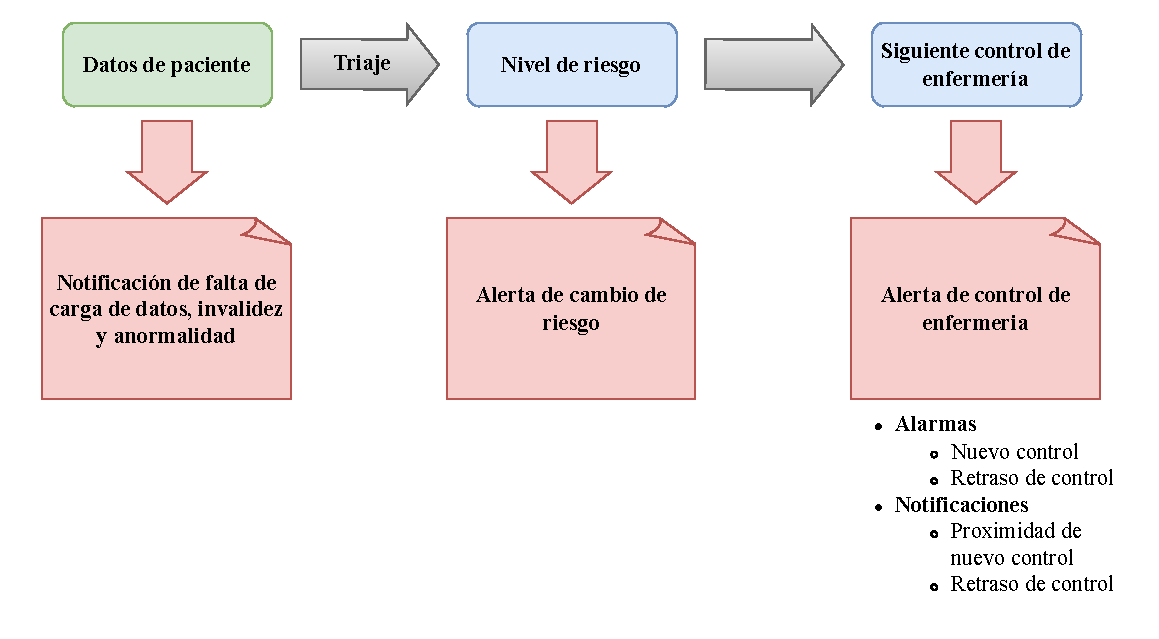
\includegraphics[width=\linewidth]{Imagenes/Intro/TransformacionDatos.pdf}
    \caption{Ingreso y transformación de los datos}
    \label{fig:transformacionDatos}
\end{figure}
El objetivo de ALERTAR es operar en una gran cantidad de hospitales. Por esto, se diseñó para garantizar su funcionamiento incluso en condiciones de conectividad limitada, adaptándose tanto a variaciones en la calidad de la conexión a Internet como a diferencias en la infraestructura de red dentro de cada sector hospitalario. Dado que se trata de un sistema crítico para la atención de pacientes, se requiere un alto grado de resiliencia. Para cumplir con este requisito, el sistema debe garantizar la comunicación entre dispositivos a través de una red de área local (LAN). Esto permite que los dispositivos sigan comunicándose y sincronizándose, asegurando el funcionamiento local del sistema aún en caso de pérdida de conexión a Internet.

Los siguientes requerimientos del sistema influyen directamente en la elección de la solución técnica: 
\begin{enumerate}
    \item Uso exclusivo de dispositivos móviles en lugar de infraestructura adicional como computadoras o servidores locales. Esto facilita la adopción y despliegue del sistema, especialmente en hospitales con recursos limitados.
    \item El sistema debe mantenerse operativo y confiable, es decir ser resiliente, ante fallos en la infraestructura de red, problemas de hardware o software. Esto es crucial debido a la importancia de garantizar la continuidad del servicio en la atención de pacientes.
    \item El alcance del sistema debe ser multi hospitalario, para permitir la recolección masiva de datos clínicos, lo cual es esencial para la calibración continua de los sistemas de alerta temprana y el incremento de la capacidad predictiva del sistema.
\end{enumerate}

Ante estos desafíos, el sistema ALERTAR fue diseñado con una arquitectura distribuida que optimiza la resiliencia frente a fallos de conectividad y hardware. La metodología adoptada en su desarrollo permite garantizar su operatividad en entornos hospitalarios con condiciones variables de red.
% Agregar solucion global
% Se propone una arquitectura distribuida en nube, niebla y borde... a partir de esto enlazo con objetivos

%Redefinir objetivos especificos cosa que coincida con lo que hice.

\section{Objetivos y alcance de la tesis}
El objetivo general de esta tesis es:

\begin{center}
    \textit{Implementar un prototipo básico del núcleo de la aplicación móvil del sistema ALERTAR.} 
\end{center}

Se considera que el núcleo de la aplicación móvil comprende toda la funcionalidad de la aplicación con excepción de la interfaz gráfica. En esta tesis se desarrolla un prototipo básico del núcleo de la aplicación móvil, compuesto por una plataforma base y un conjunto limitado de casos de uso implementados sobre ella.

La experimentación sobre este prototipo permite validar la plataforma base, e identificar posibles mejoras arquitectónicas o de implementación, con el fin de establecer una base sólida que permita completar, en etapas posteriores, la funcionalidad prevista para el dominio de la aplicación móvil.
\\\\
Para alcanzar el objetivo general se definen los siguientes objetivos específicos:
\begin{enumerate}
    \item Implementar la capa de transporte de datos de la aplicación móvil, permitiendo:
    \begin{itemize}
        \item Comunicaciones seguras, que garanticen la protección de información confidencial de pacientes. 
        \item Monitorear la conectividad de la aplicación móvil con otros componentes del sistema (dispositivos móviles y la nube) para detectar la interrupción de conexiones.
    \end{itemize}
        

    \item Implementar el mecanismo de tolerancia a fallos de la aplicación móvil basado en replicación de datos entre dispositivos móviles y la nube.

    \item Verificar el correcto funcionamiento del mecanismo de tolerancia a fallos mediante una validación funcional con casos de uso básicos del dominio, incluyendo pruebas de concurrencia.
    
    \item Realizar una evaluación del rendimiento de la aplicación móvil implementada, considerando:
    \begin{itemize}
        \item Eficiencia del almacenamiento local de datos.
        \item Tiempo de ejecución de operaciones básicas del mecanismo de tolerancia a fallos basado en replicación de datos.
    \end{itemize}

    
\end{enumerate}

%Objetivos especificos:
%- Implementar un mecanismo de toleracia a fallos basado en la replicacion de datos considerando los siguientes aspectos calve...

%- Implementar un protocolo de comunicaciones destinado a interconectar los diversos componentes que integran al sistema ALERTAR, de manera tal que se logre...

%- Relizar un marco teorico el cual sustente las decisiones de diseño y tecnologicas adoptadas.

%- Explorar como la integracion de dispositivos moviles como infraestructura hospitalaria, facilitan la gestion y aseguran la resiliencia en entornos medicos criticos

%- Explorar como la integracion del sistema ALERTAR con una arquitectura cloud-fog-edge contribuye a la eficiencia del sistema y a la mejora de la atencion medica, proporcionando una infraestructura resiliente, escalable y segura

\section{Metodología}
ALERTAR es la evolución del sistema COVINDEX \cite{chiarotto2024covindex, chiarottoJornadasCloud}, desarrollado durante la pandemia de COVID-19. Debido al contexto de urgencia sanitaria, COVINDEX fue implementado de manera apresurada y experimental, sin un diseño previo detallado, sin visión a futuro y con limitaciones en cuanto a escalabilidad, lo que lo restringe únicamente al tratamiento de casos de COVID-19.

Ante la necesidad de un sistema más generalizado, surgió la oportunidad de diseñar un sistema que asista a médicos y enfermeros en unidades de cuidados intensivos, sin limitarse a una sola patología. A partir de esta necesidad, se desarrolló el diseño arquitectónico y se establecieron los lineamientos básicos para implementar un sistema más amplio. Este trabajo de tesis se encarga del desarrollo de un prototipo básico del núcleo de la aplicación móvil del sistema ALERTAR a partir de dicho diseño.

El desarrollo del sistema ALERTAR se estructura en tres componentes principales: implementación del servidor remoto (nube), diseño e implementación de la interfaz gráfica móvil, y diseño e implementación del núcleo de la aplicación móvil, siendo el prototipo básico de este último el foco de este trabajo de tesis. El proyecto se llevó a cabo de manera colaborativa entre profesores y alumnos. En paralelo, un profesor estuvo a cargo de la implementación del componente de la nube, mientras que tres alumnos se dedicaron al desarrollo de la interfaz gráfica móvil. Esta colaboración facilitó considerablemente tanto el desarrollo como la prueba del núcleo de la aplicación móvil, permitiendo la validación y puesta en marcha de la aplicación directamente en dispositivos móviles llegando a tener a día de hoy un prototipo funcional.

\section{Trabajos relacionados}
Una aplicación que trabaja sobre el mismo dominio y tiene objetivos similares a ALERTAR es Intramed \cite{intraMed}. Intramed es una plataforma que monitorea a los pacientes dentro de un hospital, permitiendo almacenar y acceder a información clínica de los mismos. Utiliza una segunda aplicación llamada Vitals360 \cite{Vitals360} para monitorear en tiempo real los signos vitales de los pacientes. En conjunto, ambas proporcionan resultados intuitivos y sencillos para los usuarios en forma de listas y gráficos, permitiendo llevar a cabo expedientes electrónicos de los pacientes. Además, Intramed registra información relativa a médicos, enfermeros, documentos clínicos, reservas de quirófanos o laboratorios y facilita la comunicación entre profesionales a través de la escritura.

Si bien los dispositivos de Intramed, cuando pierden conexión con Internet, almacenan localmente la información y la envían una vez restablecida la conexión, estos no pueden compartir información entre sí por más que se encuentren en un mismo hospital donde podrían aprovechar, por ejemplo, la red de área local (LAN). Esto es malo dado que existe riesgo de pérdida de los datos ante fallos de dispositivos móviles y tiene impacto directo en la atención al paciente debido a la incapacidad de compartir información crucial de manera rápida y eficiente, lo que afecta al monitoreo apropiado de los pacientes. En cambio, ALERTAR cuenta con un sistema de comunicación auxiliar por red de área local para evitar la desconexión en zonas con acceso débil o nulo a Internet. Esta propiedad es vital para ofrecer un servicio crítico en la atención de pacientes.

Otra aplicación relacionada es eWeLink \cite{eWeLink}, la cual se utiliza para controlar dispositivos inteligentes para el hogar, especialmente aquellos basados en tecnología de Internet de las cosas. La aplicación permite a los usuarios controlar y monitorear dispositivos del hogar inteligente a través de dispositivos móviles, permitiendo encender o apagar luces, electrodomésticos y otros dispositivos desde cualquier lugar con conexión a Internet. eWeLink realiza una comunicación entre dispositivos similar a la de ALERTAR, ya que funciona tanto a través de Internet como por medio de una red LAN. Sin embargo, trabaja en un contexto y dominio totalmente diferente y el nivel de resiliencia es bajo debido a que la funcionalidad se ve notablemente reducida cuando no se cuenta con acceso a la red de Internet.

Por último, COVINDEX \cite{chiarotto2024covindex, chiarottoJornadasCloud} es la versión antecesora de ALERTAR, su objetivo es monitorear pacientes con COVID-19 y proporcionar alertas tempranas de gravedad. Debido al contexto de emergencia, se implementó rápidamente sin un diseño extensible, limitando su aplicación exclusivamente al COVID-19, quedando como un prototipo experimental.
%Agregar comparativa


\section{Organización del resto del trabajo}
En el capítulo \ref{cap:marcoTeorico}, se presenta el marco teórico de los elementos y fundamentos que sustentan el desarrollo del prototipo básico del núcleo de la aplicación móvil del sistema ALERTAR. En el capítulo \ref{cap:arquitecturaGeneral}, se detalla la arquitectura general del sistema, explicando los componentes que la conforman. El capítulo \ref{cap:implementacion} aborda la implementación de la aplicación móvil. En el capítulo \ref{cap:experimentacion}, se presentan los resultados de los experimentos realizados. Finalmente, en el capítulo \ref{cap:conclusionesYTrabajosFuturos}, se exponen las conclusiones derivadas del desarrollo del prototipo básico del núcleo de la aplicación móvil del sistema ALERTAR y se enumeran posibles trabajos futuros a realizar.
\chapter{Marco teórico}\label{cap:marcoTeorico}
Este capítulo plantea las bases conceptuales que sustentan las metodologías y tecnologías empleadas en el desarrollo y la implementación del núcleo del sistema ALERTAR, además de exponer las definiciones y terminología a utilizar a lo largo del trabajo de tesis. %Se comienza explorando el Protocolo de Control de Transmisión (TCP), que es fundamental para la transmisión confiable de datos en redes de computadoras. Luego, se aborda la seguridad de las comunicaciones, con un enfoque específico en el cifrado asimétrico junto con el uso de certificados de claves públicas para garantizar la confidencialidad, autenticidad e integridad de los mensajes. Después, se explora la arquitectura limpia, un enfoque que promueve un diseño de software robusto y mantenible. Finalmente, se discute la arquitectura \textit{Cloud-Fog-Edge Computing}, que representa una evolución en la computación distribuida, integrando capacidades de procesamiento y almacenamiento desde la nube hasta el borde de la red.

En la sección \ref{sec:TCP} se presenta el protocolo TCP junto con los aspectos teóricos más relevantes. En la sección \ref{sec:segDeLasComun} se detallan las propiedades necesarias para asegurar la seguridad de las comunicaciones, se describe cifrado asimétrico, certificados de claves públicas, verificación de validez de certificados y diferentes métodos para su implementación y distribución, finalizando con una explicación del protocolo \textit{TLS}. En la sección \ref{sec:arqLimpia} se describe qué es y cómo funciona una arquitectura limpia. Por último, en la sección \ref{sec:cloud-fog-edge} se describe arquitectura \textit{Cloud-Fog-Edge Computing} y se detalla la responsabilidad y funcionalidad de cada una de sus capas.
\section{TCP}
\label{sec:TCP}
TCP \textit{(Transmission Control Protocol)} es un protocolo fundamental en las redes de computadoras para la transmisión de datos. Es un protocolo orientado a la conexión, lo que implica que dos aplicaciones deben establecer una conexión previa mediante un proceso denominado ``handshake'' antes de intercambiar información. Este proceso de tres pasos asegura que ambos extremos estén sincronizados y listos para intercambiar datos de manera efectiva.

Una vez establecida la conexión, TCP garantiza la entrega ordenada de los datos mediante el uso de números de secuencia. Cada segmento de datos enviado incluye un número de secuencia que indica la posición del primer byte del segmento dentro del flujo de datos. Esto permite que los datos sean reordenados en el destino en caso de llegar fuera de orden, y que se detecten y eliminen duplicados. La transmisión ordenada es crucial para aplicaciones que requieren que los datos lleguen en el mismo orden en que fueron enviados.

TCP ofrece un servicio de \textit{full-duplex}, permitiendo que los datos fluyan simultáneamente en ambas direcciones. Cada extremo de la conexión mantiene un número de secuencia independiente para cada dirección, y los segmentos TCP incluyen un campo de reconocimiento (ACK) para confirmar la recepción de datos en la dirección opuesta \cite{tcpillustratedvol1}.

La fiabilidad es otra característica clave de TCP. En caso de pérdida de datos, TCP retransmite los segmentos no reconocidos por el receptor dentro de un tiempo determinado. Utiliza un temporizador de retransmisión que se actualiza cada vez que se recibe un ACK. Si no se recibe un ACK dentro del tiempo esperado, el segmento se retransmite. Este mecanismo asegura que todos los datos lleguen a destino sin pérdidas.

TCP utiliza una suma de comprobación para verificar la integridad de los datos transmitidos. Esta suma de comprobación se calcula sobre el encabezado TCP, los datos transmitidos y el pseudo-encabezado \textit{IP}, el cual incluye la dirección \textit{IP} de origen, la dirección \textit{IP} de destino, el protocolo y la longitud total del segmento TCP. Si se detecta un error en la suma de comprobación, el segmento de datos se descarta y no se envía ninguna confirmación para ese segmento. De esta manera TCP asegura que sólo los datos libres de errores sean aceptados y procesados.


TCP incorpora mecanismos de control de flujo y control de congestión:
\begin{itemize}
    \item \textbf{Control de Flujo: }utiliza una ventana deslizante que permite al receptor controlar la cantidad de datos que el emisor puede enviar antes de recibir una confirmación. Esto evita que el receptor se vea abrumado por una cantidad excesiva de datos.
    \item \textbf{Control de Congestión: }Ajusta dinámicamente la velocidad de transmisión de datos en función de la capacidad de la red y las condiciones actuales de congestión. Esto ayuda a prevenir la sobrecarga de la red y asegura una transmisión fluida.
\end{itemize}















%TCP \textit{(Transmission Control Protocol)}de comunicación utilizado en redes de computadoras para la transmisión de datos. Proporciona una conexión confiable y orientada a la conexión entre dos aplicaciones a través de una red. TCP garantiza la entrega ordenada y sin errores de un flujo de datos, controlando la transmisión y recepción de los paquetes de datos entre dispositivos conectados.

%El término ``orientado a conexión'' en el contexto de TCP implica que dos aplicaciones deben establecer una conexión previa mediante un proceso denominado \textit{handshake} antes de intercambiar información. Esta conexión se asemeja al saludo y apretón de manos entre dos personas antes de iniciar una conversación. En este proceso, ambas partes acuerdan establecer una conexión y se aseguran de estar listas para intercambiar información. De manera similar, en el handshake de TCP, dos dispositivos establecen una conexión, confirman su disposición para intercambiar datos y sincronizan sus estados antes de comenzar la transmisión de información. Este proceso es un paso fundamental para garantizar una comunicación efectiva y ordenada entre los sistemas.

%TCP proporciona una abstracción de flujo de bytes a las aplicaciones que lo utilizan. En consecuencia TCP no inserta automáticamente \textit{marcadores de registro} ni límites de mensajes. Un marcador de registro se corresponde a un índice del alcance de escritura de una aplicación. Si la aplicación de un lado escribe 10 bytes, seguido por la escritura de otros 20 bytes, seguidos por otros 50 bytes, la aplicación al otro lado de la conexión no puede determinar la longitud de las escrituras individuales. Por ejemplo, el receptor podría leer 80 bytes en cuatro tandas de 20 bytes, podría leerlo en tandas como se planteó originalmente o en una combinación diferente de longitudes. Cada extremo de la conexión pone un flujo de datos en TCP, y el mismo flujo de bytes aparece en el otro extremo. Cada punto de destino o \textit{end point} elige de manera particular sus tamaños de escritura y lectura.

%TCP no interpreta el contenido de los bytes dentro del flujo. Este no tiene idea de si los bytes de información son datos binarios, caracteres ASCII, caracteres EBCDIC, o de algún otro tipo. La interpretación del flujo de bytes es responsabilidad de cada extremo de la conexión \cite{tcpillustratedvol1}.

%\subsubsection{Fiabilidad en TCP} 

%Al proveer una interfaz de flujo de bytes, TCP debe convertir los flujos de bytes salientes en un conjunto de paquetes que IP pueda transportar. Esto se denomina \textit{Empaquetado}. Estos paquetes contienen números de secuencia que, en TCP, representan los desplazamientos de los bytes en el flujo de datos general, en lugar de enumerar directamente cada paquete. El número de secuencia indica la posición del primer byte del paquete dentro del flujo. Esto permite que los paquetes sean de tamaño variable durante la transferencia y también permite que se combinen, proceso el cual se denomina \textit{re-empaquetado}. Los datos de la aplicación se dividen en lo que TCP considera los fragmentos de mejor tamaño para enviar, generalmente ajustando cada segmento en un único datagrama de capa IP que no se fragmentará. Los fragmentos pasados de TCP a IP se denominan \textit{segmentos}.

%TCP realiza un control de integridad mediante una \textit{suma de comprobación (checksum)} en su encabezado, así como en cualquier dato de aplicación asociado y algunos campos del encabezado IP. Esta suma de comprobación es obligatoria y tiene como objetivo detectar posibles errores de bits que puedan haberse introducido durante la transmisión. Si un segmento llega con una suma de comprobación inválida, TCP lo descarta sin enviar ninguna confirmación para el paquete descartado. Sin embargo, el receptor TCP podría confirmar la recepción de un segmento anterior (ya confirmado) para ayudar al remitente en sus cálculos de control de congestión. La suma de comprobación utilizada por TCP es la misma función matemática utilizada por otros protocolos de Internet (UDP, ICMP, etc.)

%Cuando TCP envía un conjunto de segmentos, suele establecer un temporizador de retransmisión que espera el \textit{reconocimiento (ACK)} de recepción desde el otro extremo de la conexión. TCP no configura temporizadores de retransmisión distintos para cada segmento. En cambio, establece un temporizador al enviar una ventana de datos y actualiza el tiempo de vencimiento cada vez que recibe un ACK. Si no se recibe un ACK dentro del plazo establecido, el segmento se retransmite.

%Cuando TCP recibe información desde el extremo opuesto de la conexión, responde enviando un reconocimiento (ACK). Este reconocimiento no siempre se transmite inmediatamente, sino que usualmente es retrasado una fracción de segundo. Los ACKs utilizados por TCP son ``acumulativos'' en el sentido de que un ACK que indica el número de byte $N$ implica que todos los bytes hasta ese número $N$ (sin incluirlo) ya fueron recibidos de manera exitosa. Esto provee robustez frente a la pérdida de ACK. Si un ACK se pierde, es muy probable que un ACK posterior sea suficiente para indicar el reconocimiento de segmentos previamente enviados.

%TCP proporciona un servicio de \textit{full-duplex} a la capa de aplicación, permitiendo que la información fluya en ambas direcciones de manera independiente. En consecuencia, cada extremo de la conexión debe mantener un número de secuencia para el flujo de datos en cada dirección. Una vez establecida la conexión, cada segmento TCP que transporta información en una dirección, incluye un ACK para los segmentos en la dirección opuesta. Además, cada segmento contiene una ventana de anuncios para implementar el control de flujo en la dirección opuesta. Cuando llega un segmento TCP en una conexión, la ventana puede deslizarse hacia adelante, el tamaño de la ventana puede cambiar y nuevos datos pueden haber llegado. Este mecanismo asegura la bidireccionalidad y la independencia del flujo de datos en una conexión TCP.

%Utilizando los números de secuencia, el receptor TCP descarta los segmentos duplicados y reordena aquellos que lleguen desordenados. Esto se hace debido a que TCP utiliza IP para enviar los segmentos, e IP no provee eliminación de duplicados ni garantiza el orden correcto de recepción. Como se trata de un protocolo de flujo de bytes, TCP nunca envía información fuera de orden. Por lo tanto, el receptor TCP puede verse obligado a retener datos con números de secuencia más grandes antes de entregarlos a una aplicación hasta que se complete la recepción de un segmento como un número de secuencia inferior el cual generaba un ``hueco'' \cite{tcpillustratedvol1}.
%Investigar como objetivos de la seguridad de la información o telecomunicaciones
%Intro: Confidencialidad, autenticidad e integridad de las comunicaciones
\section{Seguridad de las comunicaciones}
\label{sec:segDeLasComun}
La seguridad de la información en telecomunicaciones es crucial para proteger los datos en tránsito. En este campo, la confidencialidad, la autenticidad y la integridad de los datos son fundamentales.

La confidencialidad implica la protección de la información sensible contra accesos no autorizados. A través de métodos como la encriptación, se busca garantizar que solo los destinatarios autorizados puedan interpretar la información transmitida, preservando así la confidencialidad de los datos \cite{stallings2016network}

La autenticidad se refiere a la verificación de la identidad de las entidades involucradas en una comunicación. Para este fin, se emplean mecanismos como la autenticación de dos factores y la firma digital, aplicados en distintos contextos. Estos métodos permiten confirmar que emisor y receptor son entidades legítimas, reduciendo el riesgo de suplantación de identidad y garantizando la autenticidad del origen de los mensajes \cite{stallings2016network}. La firma digital es una técnica criptográfica basada en criptografía asimétrica que permite verificar la integridad y autenticidad de un documento electrónico, así como garantizar el no repudio. Asegura que el contenido del documento no ha sido alterado desde su firma y que el firmante no puede negar su autoría. Este mecanismo utiliza un par de claves: una clave privada, conocida únicamente por el firmante, y una clave pública, accesible a terceros para verificar la firma.

La integridad tiene como objetivo garantizar que la información no ha sido alterada ni se ha insertado contenido no autorizado, ya sea por errores accidentales durante la transmisión o por ataques maliciosos. Para ello, se emplean técnicas como los códigos de detección y corrección de errores para fallos involuntarios, y mecanismos criptográficos como funciones hash y códigos de autenticación de mensajes (MAC) para detectar modificaciones intencionadas \cite{stallings2016network, delfsintroduction}.

Éste enfoque integral en confidencialidad, autenticidad e integridad es esencial para proteger la información en las telecomunicaciones y también contribuye a fortalecer la confianza en los sistemas y servicios digitales \cite{stallings2005cryptography,stallings2016network}.

Un campo esencial para la seguridad de la información es la criptografía, donde un mensaje en su forma original se conoce como texto claro mientras que un mensaje transformado y codificado se denomina texto cifrado. La criptografía se fundamenta en principios clave para transformar el texto claro en texto cifrado. Estos principios, presentes en todos los algoritmos de cifrado, se basan en dos operaciones generales: la sustitución, donde cada elemento en el texto claro (bit, carácter, grupo de bits) es reemplazado por otro elemento, y la transposición, donde los elementos en el texto claro se reorganizan. Es crucial que no se pierda información, es decir, que todas las operaciones sean reversibles. La mayoría de los sistemas, conocidos como sistemas de producto, emplean múltiples etapas de sustituciones y transposiciones, formando un producto de operaciones criptográficas.

El proceso de convertir el texto claro en texto cifrado se conoce como cifrado o encriptación, y el acto de restaurar el texto claro a partir del texto cifrado se denomina descifrado o desencriptación.

La forma en que se procesa el texto claro también es un factor determinante porque determina cómo se cifra y descifra la información. Un cifrado de bloque procesa los elementos de entrada en bloques, generando un bloque de salida para cada bloque de entrada. Por otro lado, un cifrado de flujo procesa continuamente los elementos de entrada, produciendo la salida elemento a elemento a medida que avanza \cite{schneier2007applied, stallings2005cryptography}.

La criptografía se clasifica según el número de claves utilizadas. La criptografía simétrica, también conocida como criptografía de clave secreta o criptografía convencional, es fundamental en la seguridad de la información. En éste enfoque, se utiliza una única clave compartida entre las partes autorizadas para cifrar y descifrar datos. La premisa básica radica en mantener esta clave en secreto, asegurando que solo aquellos que poseen dicha clave secreta puedan acceder a la información protegida. 

A partir de la Figura \ref{fig:procesoCifrado} se plantea cómo es el proceso de encriptación y desencriptación de clave simétrica. En esta, se considera que $K_i$ y $K_j$ son la misma clave secreta compartida entre el emisor y el receptor. Esta clave es utilizada por los algoritmos de encriptación y desencriptación para cifrar y descifrar el texto. Los algoritmos de encriptación y desencriptación se encargan de realizar una serie de transformaciones y sustituciones sobre el texto haciendo uso de la clave provista. Este método requiere que la distribución de la clave secreta entre las entidades participantes de la comunicación se realice a través de un canal seguro. La necesidad de un canal seguro es una desventaja del método de clave simétrica, pero a cambio, se tiene el beneficio de ser muy eficiente respecto de los recursos computacionales necesarios para los procesos de cifrado y descifrado.


\begin{figure}
    \centering
    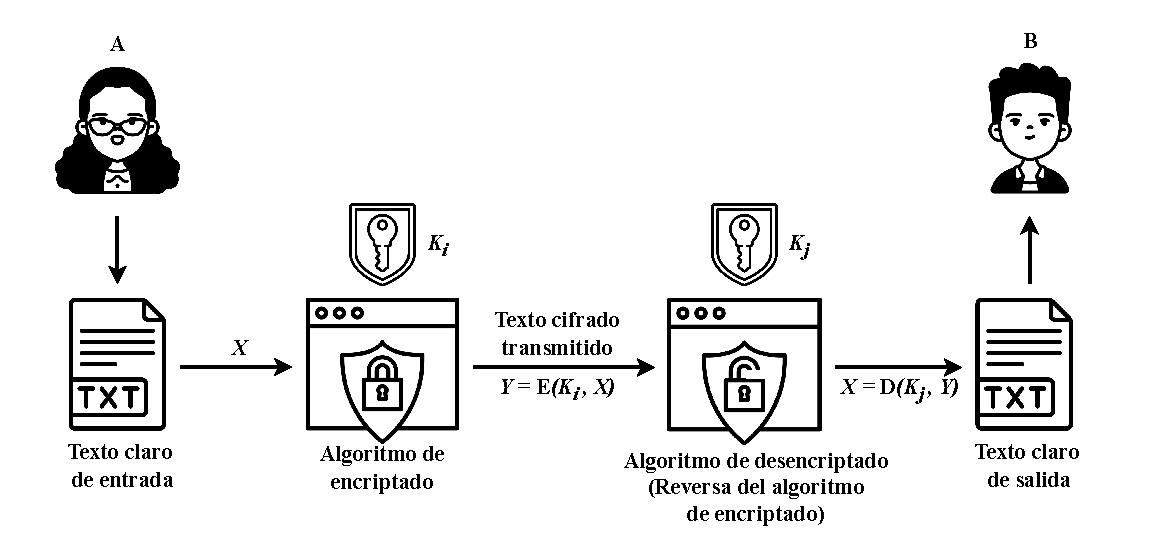
\includegraphics[width=1\linewidth]{Imagenes/Seguridad de las comunicaciones/Cifrado simetrico y asimetrico.pdf}
    \caption{Proceso de encriptación con claves}
    \label{fig:procesoCifrado}
\end{figure}

\subsection{Cifrado asimétrico}
A diferencia del cifrado simétrico, que depende de una clave secreta compartida, la criptografía de clave pública utiliza un par de claves: una \textit{clave pública} y una \textit{clave privada}. La clave pública, como su nombre lo indica, se comparte abiertamente, permitiendo que cualquiera pueda cifrar o descifrar mensajes con ella. Por otro lado, la clave privada, es secreta y solo conocida por el propietario que la generó. En este esquema, lo que se cifra con una de las claves sólo puede ser descifrado con la otra, es decir, no es posible cifrar y descifrar con la misma clave. Esto permite asegurar la confidencialidad de los mensajes, ya que un mensaje cifrado con la clave pública de un usuario sólo puede ser leído por quien posee la clave privada correspondiente.

El funcionamiento esencial para garantizar la confidencialidad se puede ver representado en la Figura \ref{fig:procesoCifrado}, donde $K_i$ es la clave pública de ``B'' y $K_j$ es la clave privada de ``B'' y se describe de la siguiente manera:
\begin{enumerate}
    \item Los usuarios generan pares de claves pública y privada. 
    
    \item Los usuarios obtienen la clave pública del otro con el que se quieren comunicar.

    \item Si ``A'' quiere enviar un mensaje confidencial a ``B'', ``A'' encripta el mensaje utilizando la clave pública de ``B''.

    \item Cuando ``B'' recibe el mensaje, éste lo desencripta utilizando su clave privada. Ninguna otra persona puede desencriptar el mensaje porque solamente ``A'' conoce su clave privada. 
\end{enumerate}

De esta manera, como cualquiera tiene acceso a las claves públicas, se elimina la necesidad de claves secretas compartidas. Siempre que la clave privada de un usuario se mantenga en secreto, la comunicación estará segura. Por otro lado, en caso de necesidad ya sea porque se filtró una clave privada u otra razón, un sistema o usuario puede generar un nuevo par de claves.

Por otro lado existe la necesidad de que los mensajes y documentos electrónicos cuenten con un equivalente a las firmas utilizadas en documentos en papel. Esto se logra con firmas digitales. 

La firma digital de un documento se realiza, de manera conceptual, de la siguiente manera:

\begin{enumerate}
    \item Si ``A'' quiere firmar un mensaje, primero genera un resumen criptográfico del mensaje (mediante una función hash). Luego, cifra ese resumen utilizando su clave privada. El resultado se adjunta al mensaje como su firma digital.

    \item Cuando ``B'' recibe el mensaje junto con la firma, genera él mismo el resumen criptográfico a partir del mensaje recibido. Luego, utiliza la clave pública de ``A'' para descifrar la firma y así obtener el resumen original. Si ambos resúmenes coinciden, se confirma que el mensaje no ha sido alterado y que fue firmado por ``A''.
\end{enumerate}

Cabe destacar que en este ejemplo el mensaje no se cifra, por lo que la firma digital no garantiza la confidencialidad, sino la autenticidad, la integridad y el no repudio del mensaje.

Este esquema garantiza tanto la autenticidad del origen, ya que solo ``A'' posee la clave privada, como la integridad del mensaje, dado que cualquier alteración modificaría el resumen y anularía la verificación de la firma.

La firma digital de un documento se realiza, de manera conceptual, de la siguiente manera:

\begin{enumerate}
    \item Si ``A'' quiere firmar un mensaje, ``A'' encripta el mensaje utilizando su clave privada.

    \item Cuando ``B'' recibe el mensaje, éste lo desencripta utilizando la clave pública de ``A''. Dado que el mensaje fue encriptado con la clave privada de ``A'', solo ``A'' pudo haberlo generado. 
\end{enumerate}

Este esquema planteado asegura que el mensaje no sea alterado sin acceso a la clave privada de A, garantizando así tanto la autenticidad del origen como la integridad del contenido del mensaje.

\subsection{Certificados de claves públicas y verificación de validez de certificados}

%Los certificados de claves públicas permiten asociar una identidad con una clave pública, proporcionando un medio para validar la legitimidad de las entidades y prevenir suplantaciones de identidad durante las transmisiones.

%\label{sec:dirPubCAyCerts}
%Los directorios de claves públicas sirven como repositorios (centralizados o distribuidos) donde los usuarios pueden buscar y obtener claves públicas de otros participantes. Estos facilitan la distribución de claves públicas y respaldan la autenticidad e integridad de las comunicaciones. Al proporcionar un medio para la consulta y verificación de claves públicas, contribuyen a establecer una red de confianza entre los usuarios. 

%Tanto el mantenimiento como la distribución del directorio público es responsabilidad de una entidad u organización externa, a la cual se la denomina autoridad de clave pública o autoridad certificante. 

%El funcionamiento de un directorio público se describe de la siguiente manera:

%\begin{enumerate}
%    \item La autoridad de clave pública mantiene un directorio con un registro que contiene el nombre y la clave pública de cada participante.
%    \item Cada participante registra su clave pública en el directorio público. Este registro debe ser realizado en persona o a través de algún canal de comunicaciones seguro que garantice la autenticidad.
%    \item Los participantes pueden reemplazar claves públicas ya existentes por una nueva cuando lo deseen. Por lo general esto se desea hacer cuando una clave pública fue utilizada para una gran cantidad de datos, evitando así ataques criptoanalíticos, o porque la clave privada asociada se vio comprometida de alguna manera.
%    \item Los participantes acceden de manera electrónica al directorio público. Para hacer esto de manera segura, es necesario que la comunicación entre la autoridad y el participante sea autenticada y segura, y que la clave pública de la autoridad sea obtenida previamente de una fuente confiable, ya sea en persona o a través de un canal de comunicaciones seguro, para garantizar la autenticidad de la autoridad.
%\end{enumerate}

%Para lograr un mayor nivel de seguridad se puede realizar un control más estricto sobre la distribución de las claves. En la Figura \ref{fig:directorioPK} se plantea un escenario donde se asume que una autoridad central mantiene un directorio dinámico de claves públicas de todos los participantes. Además cada participante conoce, y obtiene a través de un canal seguro, la clave pública de la autoridad y dicha autoridad es la única que conoce su propia clave privada. De esta manera se describe el siguiente proceso:

%\begin{figure}
%    \centering
%    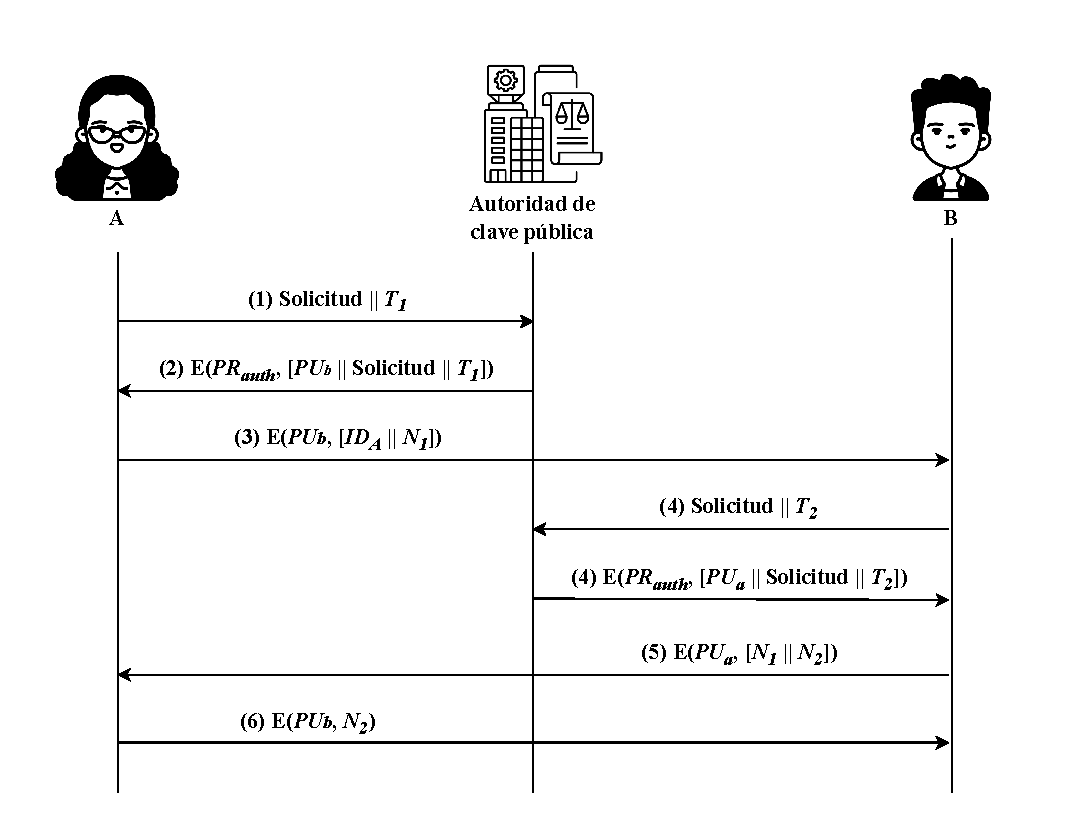
\includegraphics[width=\textwidth]{Imagenes/Seguridad de las comunicaciones/Certificados.pdf}
%    \caption{Escenario de distribución de claves públicas con entidad certificante}
%    \label{fig:directorioPK}
%\end{figure}
%\begin{enumerate}
%    \item ``A'' envía un mensaje de solicitud con marca de tiempo a la autoridad de clave pública pidiendo la clave pública de ``B''.
%    \item La autoridad responde con un mensaje firmado digitalmente con su clave privada. Por lo tanto, ``A'' está segura de que el mensaje fue emitido por la autoridad. El mensaje por parte de la autoridad contiene la siguiente información:
 %   \begin{itemize}
 %       \item Clave pública de ``B'', $PU_b$.
 %       \item La solicitud original. De esta manera ``A'' puede comparar la respuesta con la solicitud original y verificar que no fue adulterada antes de la recepción por parte de la autoridad.
 %       \item La marca de tiempo original. Con esta ``A'' puede determinar si se trata de un mensaje viejo de la autoridad cifrado con otra clave diferente a la clave pública actual de ``B''.
%    \end{itemize}
 %   \item ``A'' almacena la clave pública de ``B'' y la utiliza para encriptar un mensaje con destino a ``B'', agregando su identificador $ID_A$ y un número único ($N_1$), el cual es utilizado para identificar unívocamente la transacción.
 %   \item Utilizando el mismo mecanismo, en caso de ser necesario, ``B'' obtiene la clave pública de ``A''.

%\end{enumerate}
%De esta manera, las claves públicas fueron distribuidas de forma segura tanto a ``A'' como a ``B'', y pueden comenzar un intercambio de información seguro. Finalmente se tienen dos pasos opcionales los cuales verifican que efectivamente ``A'' y ``B'' se están comunicando entre ellos y la clave pública no fue falsificada.
%\begin{enumerate}
%\setcounter{enumi}{4}
%    \item ``B'' envía un mensaje a ``A'', encriptado con la clave pública de esta, es decir $PU_a$, este mensaje contiene el número único de ``A'' ($N_1$) así como un nuevo número único generado por ``B'' ($N_2$). Como solamente ``B'' pudo haber desencriptado el mensaje del paso 3, dado que para ello se requería utilizar su clave privada, la presencia de ($N_1$) en el mensaje de este paso le asegura a ``A'' que el emisor es ``B''.
%    \item ``A'' retorna ($N_2$), el cual es encriptado con la clave pública de ``B'', para asegurarle a ``B'' que el mensaje efectivamente fue emitido por ``A''.
%\end{enumerate}

%De los 6 pasos planteados, los primeros 4 primeros se realizan de forma poco frecuente ya que tanto ``A'' como ``B'' pueden guardar las claves públicas para usos futuros. De todas maneras, es recomendable que los usuarios soliciten periódicamente copias ``frescas'' de claves públicas a sus autoridades correspondientes.



Para garantizar comunicaciones seguras en redes abiertas, es necesario asociar de forma confiable una clave pública con la identidad de su propietario. Esta asociación se logra mediante los \textit{certificados digitales}, que permiten a los usuarios verificar la legitimidad de las claves públicas sin necesidad de consultar constantemente a una autoridad central.

Un certificado digital está compuesto, en esencia, por una clave pública y un identificador del dueño de la clave. Estos elementos conforman un bloque de información que es firmado por un tercero de confianza utilizando su propia clave privada. Típicamente, este tercero es una autoridad certificante (CA), como agencias gubernamentales o instituciones financieras reconocidas por la comunidad.

En la Figura \ref{fig:CADist} se puede ver un ejemplo de emisión de certificados, en esta, los usuarios presentan sus claves públicas a la autoridad a través de un medio seguro con el objetivo de obtener un certificado. La autoridad genera y firma el certificado, representado en la figura con las expresiones del tipo $E(PR_{auth},[T_1||ID_A||PU_a])$, y lo entrega a través del mismo medio. Luego, el usuario puede publicar o compartir este certificado. Cualquier otro que requiera de la clave pública del usuario puede obtener el certificado y verificar que este sea válido mediante la firma adjunta de la entidad certificante haciendo uso de una copia propia de la clave pública de la misma entidad. Además, a los certificados se les asigna una marca de validez temporal. Si una entidad certificante cambia su clave privada, deberán actualizarse todos los certificados firmados con esta.

\begin{figure}
    \centering
    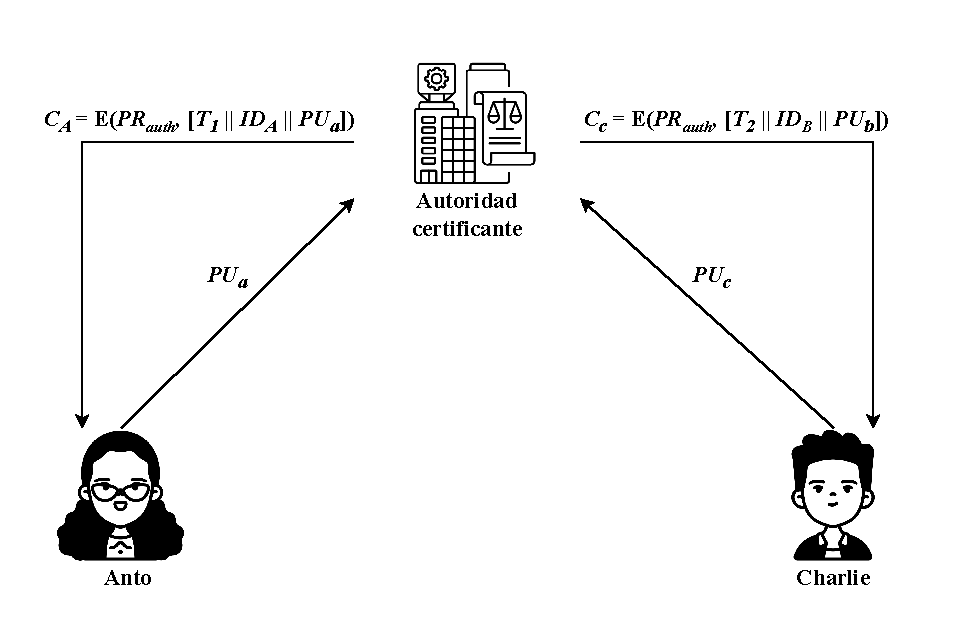
\includegraphics[width=\textwidth]{Imagenes/Seguridad de las comunicaciones/EntidadCertificante.pdf}
    \caption{Distribución de certificados desde la autoridad certificante}
    \label{fig:CADist}
\end{figure}

\textbf{Existen dos tipos principales de autoridades certificantes:}

\begin{itemize}
    \item \textit{Autoridad Certificante Pública:} Es una entidad reconocida globalmente (por ejemplo, por navegadores y sistemas operativos), que emite certificados confiables sin requerir configuración adicional por parte de los usuarios.
    \item \textit{Autoridad Certificante Privada:} Emite certificados dentro de una organización o sistema cerrado. Su uso requiere que los sistemas clientes confíen explícitamente en su clave pública. Se utilizan en entornos corporativos o internos.
\end{itemize}


El uso de certificados digitales da lugar a diferentes configuraciones de infraestructuras de claves públicas como por ejemplo \cite{chokhani2003internet, linn2000trust}:
\begin{itemize}
    \item \textbf{\textit{PKI} Jerárquica:} Hay una autoridad raíz que es la entidad más confiable y, debajo de ella, existen varias entidades subordinadas. Esta configuración permite la delegación de responsabilidades a través de una cadena de confianza establecida a través de certificados.
    \item \textbf{\textit{PKI} en Malla:} Varias entidades certificantes están interconectadas y se reconocen mutuamente, creando una red de confianza, siendo más flexible y descentralizada que las \textit{PKI} jerárquicas ya que no existe una única entidad central.
\end{itemize}

Los certificados autofirmados son generados y firmados por la propia entidad que los utiliza, sin la intervención de una entidad certificante externa. Estos certificados son útiles en entornos propios, donde se requiere cifrado pero no se necesita la verificación por una entidad de confianza externa. En estos entornos, aunque cualquier entidad pueda crear un certificado autofirmado, la autenticidad y seguridad de las comunicaciones se mantienen al confiar en la infraestructura interna de la organización \cite{kumar2019security, cooper2008internet}.


%Por otro lado existen los denominados \textit{certificados autofirmados}, los cuales no son emitidos por una entidad certificante externa, sino que son generados y firmados por la propia entidad que los utilizará. Estos certificados son útiles en situaciones donde se necesita cifrado pero no se requiere la verificación por una entidad de confianza externa. El hecho de que cualquier entidad pueda crear un certificado auto firmado compromete la autenticidad y seguridad de la comunicación, ya que no hay una entidad confiable que valide la autenticidad del certificado. Para mitigar estos riesgos, se pueden implementar infraestructuras de clave pública interna o utilizar mecanismos como el \textit{pinning} para garantizar que solo los certificados específicos y esperados sean aceptados por la aplicación.

\subsubsection{Método de verificación segura mediante pinning de certificados}
La técnica denominada \textit{pinning} permite especificar exactamente en qué entidades se puede confiar, esto a través de la comparación de certificados. Para esto se deben realizar los siguientes pasos:

\begin{enumerate}
    \item \textbf{Almacenamiento del certificado de confianza: }El receptor almacena previamente un certificado de confianza o un hash\footnote{En criptografía, un hash es una función que convierte una entrada arbitraria en una cadena de caracteres de longitud fija.} de ese certificado que recibió a través de un canal seguro.
    \item \textbf{Envío del certificado por el emisor: }Cuando el emisor inicia una conexión, envía su certificado digital al receptor para su validación.
    \item \textbf{Verificación y coincidencia: }El receptor verifica el certificado recibido comparándolo con el certificado de confianza almacenado. Si el certificado enviado por el emisor coincide con el certificado almacenado, se verifica la autenticidad de la conexión. Si no coincide, la conexión se rechaza, previniendo así ataques de hombre en el medio o suplantaciones
\end{enumerate}

Este método asegura que el receptor confía únicamente en un conjunto específico de certificados, lo cual añade una capa extra de seguridad en las comunicaciones. El \textit{pinning} es particularmente útil en aplicaciones sensibles donde la seguridad es crítica y se necesita prevenir ataques que explotan vulnerabilidades en la cadena de confianza de los certificados \cite{stallings2005cryptography, ristic2014bulletproof}.


\subsection{Transport Layer Security (TLS)}
\label{sec:TLS}
TLS es un protocolo criptográfico diseñado para proveer una comunicación segura sobre una infraestructura insegura garantizando:

\begin{enumerate}
    \item \textbf{Confidencialidad: }Mediante el uso de cifrado, TLS intenta garantizar que los datos transmitidos entre el cliente y el servidor no puedan ser interpretados por terceros no autorizados.
    \item \textbf{Integridad: }Mediante el uso de mecanismos criptográficos, como cifrados \textit{AEAD (Authenticated Encryption with Associated Data)}, TLS intenta asegurar que los datos no hayan sido alterados, ni creados, durante la transmisión.
    \item \textbf{Autenticidad: }A través del uso de certificados digitales y la autenticación del servidor, TLS verifica la identidad de las partes que se comunican, asegurando que se está hablando con la entidad correcta.
\end{enumerate}

En la Figura \ref{fig:OSI} se muestra el modelo de Interconexión de Sistemas Abiertos (OSI), un modelo conceptual utilizado para describir cómo se comunican los sistemas en red. Este modelo organiza sus funciones en siete capas jerárquicas, donde cada capa se apoya en los servicios de la inferior. La capa más baja se encarga de la transmisión física de datos, mientras que la capa más alta, la de aplicación, es la que interactúa directamente con el software del usuario y gestiona los datos de las aplicaciones. De esta manera, los protocolos no necesitan preocuparse por la funcionalidad implementada por las capas inferiores. Además, los protocolos en diferentes capas pueden agregarse y eliminarse. Un protocolo en una capa inferior puede ser utilizado por muchos protocolos de niveles superiores. 

\begin{figure}
    \centering
    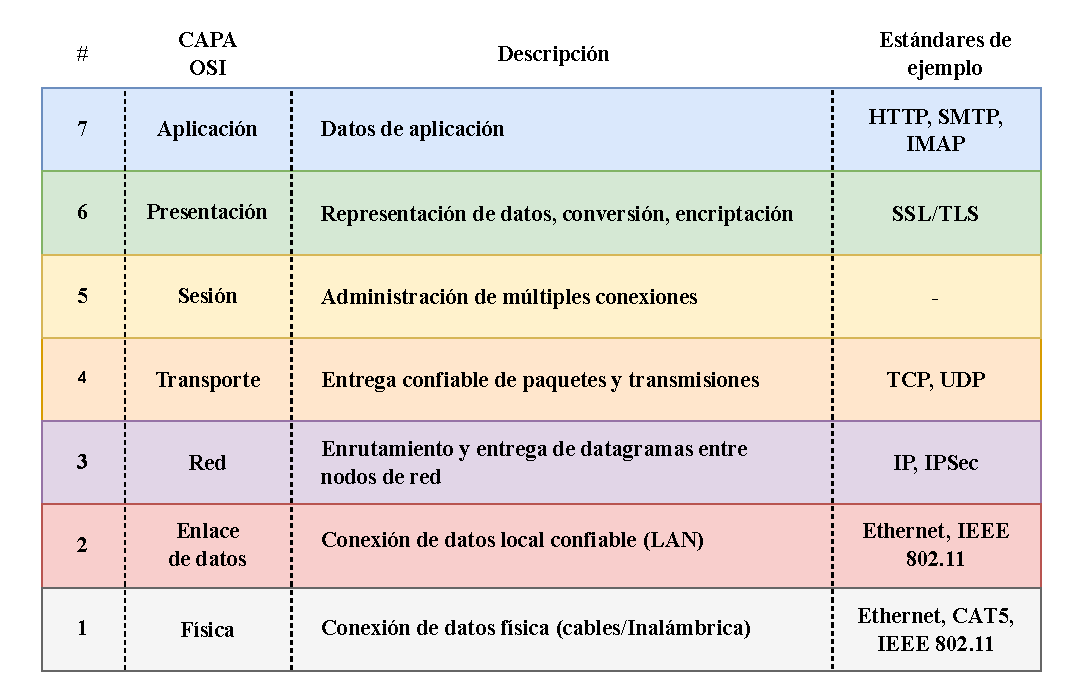
\includegraphics[width=1\linewidth]{Imagenes/Seguridad de las comunicaciones/OSI.pdf}
    \caption{Modelo de Interconexión de Sistemas Abiertos (OSI)}
    \label{fig:OSI}
\end{figure}


Así TLS se sitúa por encima de TCP pero por debajo de protocolos de nivel superior como HTTP pudiéndose utilizar para cifrar HTTP, pero también cualquier otro protocolo que trabaje sobre TCP, como SMTP o IMAP. Cuando no es necesario el cifrado, se puede eliminar TLS del modelo, de manera tal que no afecte a los protocolos de nivel superior, que continuarán funcionando sobre TCP. \cite{ristic2014bulletproof}. 

Aunque hasta aquí se ha utilizado el modelo OSI para describir la arquitectura de red, en la práctica el modelo TCP/IP es el más utilizado. Este modelo, más simplificado y representado en la figura \ref{fig:tcp_ip-tls}, no contempla explícitamente una capa de seguridad. Por esta razón, TLS se suele ubicar entre las capas de aplicación y transporte, actuando como una capa adicional de seguridad superpuesta a la capa de transporte. Esto permite que protocolos como HTTP se ejecuten de forma segura, mejorando así las capacidades del modelo TCP/IP \cite{tracy2002guidelines}.

\begin{figure}
    \centering
    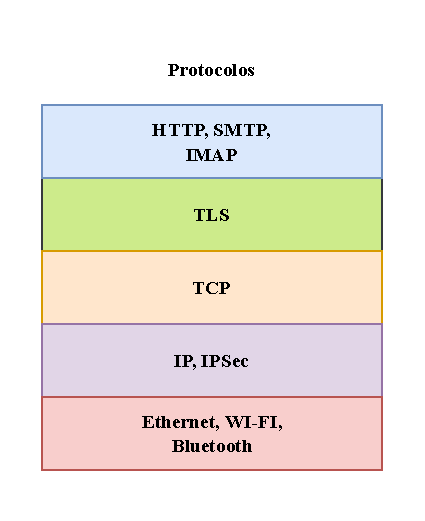
\includegraphics[width=0.5\linewidth]{Imagenes/Seguridad de las comunicaciones/TCP_IP-TLS.pdf}
    \caption{Ubicación de SSL/TLS en la pila de protocolos de Internet}
    \label{fig:tcp_ip-tls}
\end{figure}

Los principios de diseño del protocolo TLS se definen como \cite{ristic2014bulletproof}:
\begin{itemize}
    \item \textbf{Interoperabilidad: }Programadores independientes deben ser capaces de desarrollar programas y librerías que son capaces de comunicarse con otras utilizando parámetros criptográficos comunes, garantizando así la compatibilidad entre versiones TLS. La adopción de estándares abiertos y ampliamente aceptados facilita esta interoperabilidad.
    
    %Esto asegura que las distintas implementaciones de TLS sean compatibles entre sí. La adopción de estándares abiertos y ampliamente aceptados facilita esta interoperabilidad, garantizando que las aplicaciones puedan negociar y abordar protocolos, algoritmos y configuraciones de seguridad compatibles, sin importar su origen o entorno de desarrollo
    \item \textbf{Extensibilidad: }TLS tiene una arquitectura flexible que permite actualizar los algoritmos de cifrado y hash que utiliza, sin necesidad de rediseñar el protocolo completo.

    \item \textbf{Eficiencia: }TLS permite seleccionar algoritmos de cifrado y hash eficientes, lo que ayuda a minimizar el impacto de las operaciones criptográficas en el desempeño del sistema.

\end{itemize}

Toda conexión TLS comienza con un \textit{handshake}. Si el cliente nunca estableció una sesión con el servidor, ambos lados van a ejecutar un \textit{handshake} completo para negociar una \textit{sesión TLS}. Una sesión TLS es el conjunto de parámetros de seguridad acordados entre un cliente y un servidor tras completar un \textit{handshake}. Incluye la versión de TLS utilizada, el conjunto completo de algoritmos de cifrado seleccionado y las claves criptográficas que se usarán durante la comunicación. Una vez establecida, la sesión permite transmitir datos de manera segura mediante cifrado simétrico, garantizando la confidencialidad e integridad de los mensajes. Las sesiones pueden ser efímeras (válidas por una sola conexión) o reanudables, si ambas partes acuerdan reutilizar ciertos parámetros en futuras conexiones para reducir el tiempo de establecimiento.

Durante el \textit{handshake} TLS se realiza un intercambio de claves, cuyo objetivo es establecer una clave simétrica compartida entre cliente y servidor. Para lograrlo, se utiliza criptografía asimétrica o técnicas de intercambio seguro. Estas permiten que ambas partes acuerden una clave sin necesidad de transmitirla directamente. Una vez establecida esta clave simétrica, se emplea el cifrado simétrico para proteger la sesión, ya que este tipo de cifrado es mucho más eficiente computacionalmente para grandes volúmenes de datos. La criptografía asimétrica, se limita a la fase inicial de establecimiento de la sesión, debido a su mayor carga computacional.

Para negociar una nueva \textit{sesión TLS}, el cliente y el servidor realizan las siguientes cuatro actividades:

\begin{enumerate}
    \item Intercambio de capacidades y acuerdo de los parámetros de conexión deseados.
    \item Validación de los certificados presentados o autenticación mediante otros medios.
    \item Acuerdo de un \textit{secreto maestro} compartido entre ambas partes, el cual será utilizado para el cifrado durante la sesión, esta clave es denominada clave de sesión.
    \item Verificar que los mensajes emitidos durante el \textit{handshake} no fueron modificados por un tercero.
\end{enumerate}

En caso de que el cliente ya haya establecido una sesión previa con el servidor, y ambos conservan los datos necesarios, pueden realizar un \textit{handshake} abreviado, reduciendo el tiempo y el consumo de recursos. En la Figura \ref{fig:handshakeTLS} se puede observar el proceso de \textit{handshake} completo donde se describen los mensajes del protocolo.

\begin{figure}
    \centering
    \includegraphics[width= \textwidth]{Imagenes/Seguridad de las comunicaciones/handshakeTLS.pdf}
    \caption{Intercambio de mensajes del \textit{handshake} TLS. Figura extraída de} \cite{ristic2014bulletproof}.
    \label{fig:handshakeTLS}
\end{figure}
\begin{enumerate}
    
    \item \textbf{ClientHello: } Es utilizado para comunicar las capacidades del cliente y sus preferencias al servidor. Siempre es el primer mensaje de cualquier \textit{handshake} TLS. Los clientes envían este mensaje al inicio de nuevas conexiones, cuando intentan renegociar por propia decisión o en respuesta a solicitudes de renegociación por parte del servidor. A partir de este mensaje el servidor elige la versión TLS y el conjunto de cifrado que se va a utilizar en la comunicación. Cabe aclarar que TLS 1.3 eliminó la renegociación, por lo que solo TLS 1.2 y anteriores lo permiten.

    \item \textbf{ServerHello: }El propósito del mensaje \texttt{ServerHello} es comunicar los parámetros de conexión seleccionados por parte del servidor al cliente.



    \item \textbf{Certificate: }El mensaje \texttt{Certificate} se utiliza para enviar una cadena de certificados X.509 \cite{housley1999rfc2459}. Generalmente es enviado por el servidor para permitir su autenticación por parte del cliente. La cadena de certificados incluye, en orden, el certificado del servidor, los intermedios y, opcionalmente, el certificado raíz. Cada certificado en la cadena depende del siguiente para verificar su validez, por lo que la omisión de alguno puede impedir la autenticación.

    Este mensaje es obligatorio cuando el conjunto de algoritmos utilizados requiere autenticación basada en certificados, como ocurre en la mayoría de los casos para autenticar al servidor. Si el cliente no recibe el certificado y no lo tiene almacenado previamente (por ejemplo, mediante una estrategia de pinning), no podrá autenticar al servidor, comprometiendo así una de las propiedades fundamentales de TLS.
    
    Además, el mensaje \texttt{Certificate} también puede ser enviado por el cliente, si el servidor lo solicita, para realizar autenticación mutua mediante certificados.


    \item \textbf{ServerKeyExchange: }El propósito del mensaje \texttt{ServerKeyExchange} es transportar información adicional necesaria para el intercambio de claves. Su contenido varía y depende del conjunto de cifrado negociado.

    \item \textbf{ServerHelloDone: }Es una señal de que el servidor ya envió todos sus mensajes correspondientes al \textit{handshake}. Después de esto, el servidor espera mensajes por parte del cliente.

    \item \textbf{ClientKeyExchange: }Contiene la información relativa al intercambio de claves por parte del cliente. Es obligatorio y su contenido varía y depende del conjunto de cifrado negociado. Una vez recibido por parte del servidor se procede con la generación de las claves de sesión.

    \item \textbf{ChangeCipherSpec: }Es una señal de que el emisor obtuvo la información suficiente para construir los parámetros de conexión, generar las claves de sesión, y proceder con la encriptación. Tanto el cliente como el servidor envían este mensaje.

    \item \textbf{Finished: }Indica que el \textit{handshake} está completo. El cliente envía un código de autenticación de mensajes (MAC) \cite{bellare1996keying, stallings2005cryptography} de todos los mensajes del protocolo de enlace TLS que ha enviado y recibido hasta ese punto. Esto con el objetivo de verificar la integridad y la autenticidad de todos los mensajes intercambiados durante el proceso de \textit{handshake}.
\end{enumerate}

Una vez establecido el \textit{handshake} de TLS, las comunicaciones entre el cliente y el servidor quedan cifradas y seguras.


%Esto genérico y luego se desarrolla más sobre la aplicación
\section{Arquitectura limpia}
\label{sec:arqLimpia}
La arquitectura limpia, propuesta por Robert C. Martin \cite{martin2017clean}, se centra en la separación de responsabilidades y la creación de sistemas independientes de \textit{frameworks} de desarrollo de software y componentes externos. Esta metodología organiza el software en capas, con al menos una capa para las reglas de negocio y otra para interfaces de usuario y sistema.


El hecho de que las distintas capas sean independientes de los \textit{frameworks} permite utilizarlos como herramientas y no como estructuras rígidas. Esto evita que el sistema quede acoplado a sus restricciones. Además, es verificable ya que las reglas de negocio pueden ser evaluadas sin depender de la interfaz de usuario, la base de datos u otros elementos externos. Al ser una estructura modularizada en capas débilmente acopladas, los desarrolladores pueden validar, actualizar o reemplazar componentes individuales sin causar un impacto significativo en el resto del sistema. Esta flexibilidad reduce tiempos y costos de desarrollo. 

La independencia de la interfaz de usuario \textit{(UI por sus siglas en inglés)} es fundamental. Cambios en esta pueden realizarse fácilmente sin afectar al resto del sistema. La arquitectura limpia también garantiza independencia de la base de datos, la cual se considera un agente externo al igual que la interfaz de usuario. Es posible cambiar entre diferentes sistemas de gestión de bases de datos sin que las reglas de negocio estén atadas a una base de datos específica.

Por último, las reglas de negocio son independientes de cualquier agente externo. Esto significa que no tienen conocimiento de las interfaces hacia el mundo exterior. Esta separación permite una mayor flexibilidad y mantenimiento del sistema a lo largo del tiempo.

Los círculos en la Figura \ref{fig:cleanArch} representan diversas áreas de software. Teniendo en cuenta la figura, la regla clave para el funcionamiento de la arquitectura limpia es la regla de dependencia: \textit{``Las dependencias del código deben apuntar solo hacia adentro, hacia las políticas de más alto nivel''}\cite{martin2017clean}. En otras palabras, los círculos internos no deben conocer nada sobre los círculos externos. Específicamente, en el código interno no se debe mencionar el nombre de algo declarado en un círculo externo, ya sean funciones, clases, variables u otras entidades de software. La idea es que ningún cambio sobre los círculos externos tenga impacto sobre los círculos internos. Por otro lado, saltarse capas puede complicar la arquitectura, hacerla menos comprensible y más difícil de mantener, por lo que se recomienda no saltarse capas para mantener una estructura lo más clara y coherente posible.

\begin{figure}
    \centering
    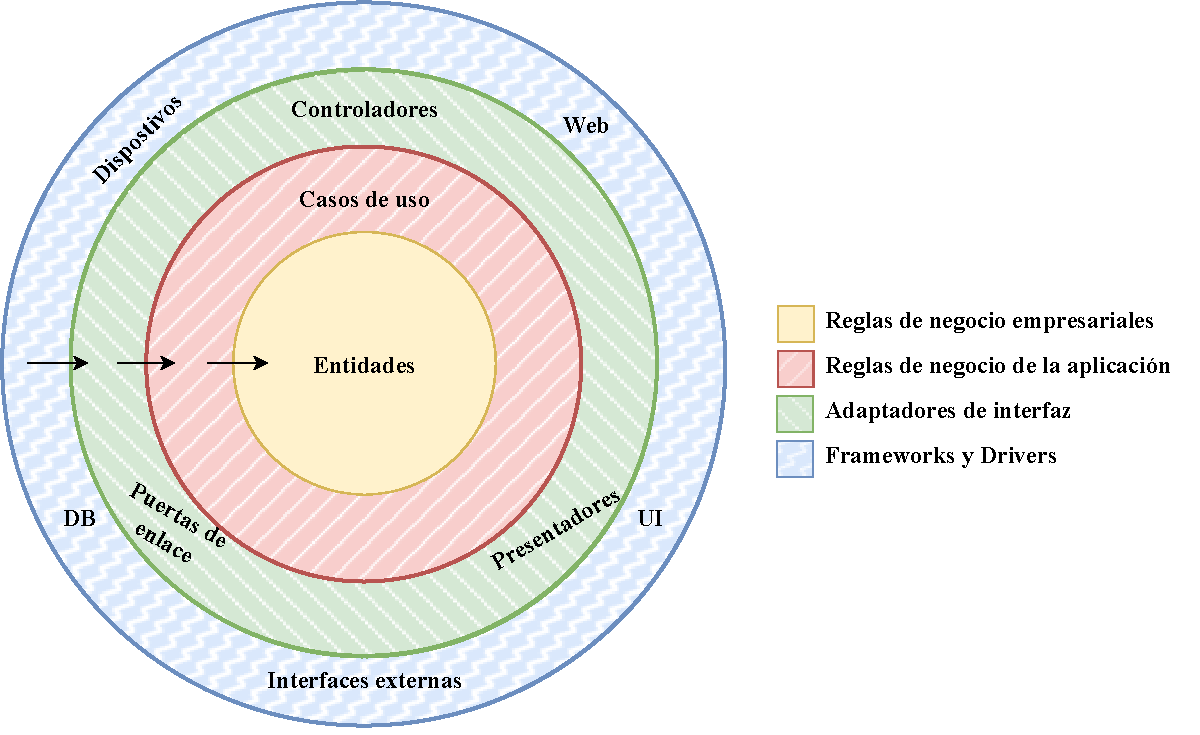
\includegraphics[width=\textwidth]{Imagenes/Arquitectura de la aplicacion movil/Arquitectura Limpia.pdf}
    \caption{Arquitectura limpia}
    \label{fig:cleanArch}
\end{figure}

Si bien la Figura \ref{fig:cleanArch} muestra cuatro círculos, no existe ninguna regla que restrinja a la utilización de estas cuatro capas siempre y cuando se aplique la regla de dependencia. Además, se debe considerar que a medida que se va hacia adentro los niveles de abstracción y políticas de alto nivel incrementan. Por otro lado, los círculos exteriores son más generales porque abordan implementaciones y detalles concretos, como las tecnologías, herramientas y componentes específicos utilizados en el sistema.

A continuación se describen las responsabilidades de cada una de las capas mostradas en la Figura \ref{fig:cleanArch}:

\begin{itemize}
    \item \textbf{Reglas de negocio empresariales: } Representan objetos de negocio fundamentales de la aplicación. Encapsulan reglas generales y de alto nivel, siendo las menos propensas a cambiar ante modificaciones externas. Una entidad puede ser un objeto con métodos, o puede ser un conjunto de estructuras de datos y funciones. Ningún cambio operativo de una aplicación específica debería afectar la capa de entidades. Por ejemplo, cambios en la interfaz de usuario de una aplicación móvil o en la seguridad no deberían afectar a estos objetos.
    \item \textbf{Reglas de negocio de aplicación: }Encapsula e implementa todos los casos de uso del sistema. Los casos de uso orquestan el flujo de datos hacia y desde las entidades, dirigiendo a dichas entidades para que utilicen sus reglas críticas de negocios y logren los objetivos del caso de uso.

    Se espera que los cambios en las reglas de negocio empresariales afecten a los casos de uso y, por lo tanto, al software de esta capa. Si los detalles en cuanto al funcionamiento relativo a un caso de uso cambian, se puede afirmar que algún código en esta capa se verá afectado.
    
    \item \textbf{Adaptadores de interfaz: }Convierten datos desde el formato más conveniente para los casos de uso y las entidades, al formato más conveniente para alguna entidad externa, y viceversa.

    \item \textbf{\textit{Frameworks} y controladores: }Generalmente está compuesta por \textit{frameworks} y herramientas como la base de datos. Es donde van todos los componentes específicos de implementación que pueden variar y ser reemplazados sin afectar la lógica central del negocio. Este tipo de componentes se mantienen en el exterior minimizando el riesgo de que cualquier cambio o problema en ellos afecte el núcleo del sistema.
\end{itemize}
%Aclaro que no hay consenso en la parte de computo en el borde
%Hacer comparativa entre diferentes perspectivas y definiciones
%Llegar a una definición propia
%Cloud-fog-device podria ser una definición
\section{Arquitectura \textit{Cloud-Fog-Edge Computing}} 
\label{sec:cloud-fog-edge}
La arquitectura cloud-fog-edge representa un enfoque integral para la distribución y gestión eficiente de recursos en entornos distribuidos y heterogéneos. Este paradigma aborda las demandas crecientes de aplicaciones modernas, que requieren procesamiento de datos cercano al punto de generación, así como la capacidad de escalar dinámicamente y aprovechar recursos ubicados de manera remota como lo puede ser una nube.

En este contexto, la arquitectura representada en la Figura \ref{fig:fog} se despliega en tres capas distintas: la nube \textit{(cloud)}, la niebla \textit{(fog)} y el {borde \textit{(edge)}, cada capa tiene características y funcionalidades únicas que se adaptan a diferentes necesidades y restricciones de las aplicaciones y dispositivos.

\begin{figure}
    \centering
    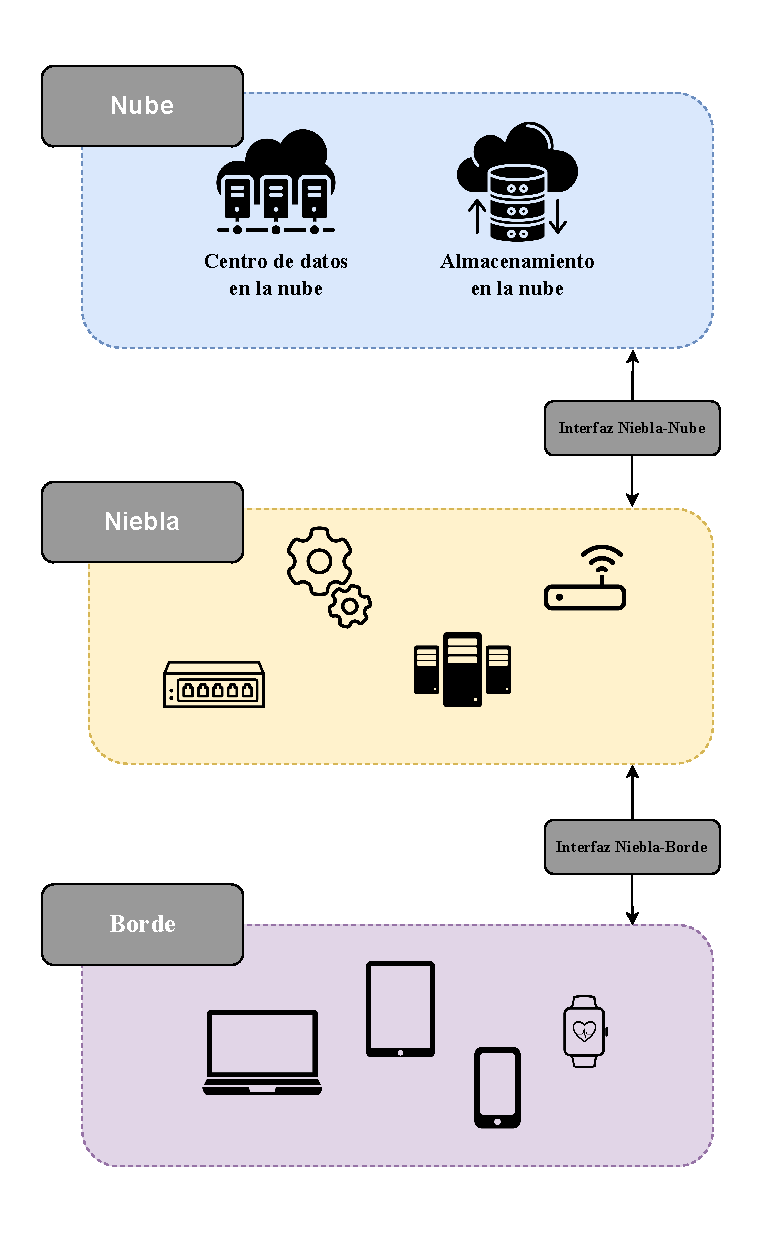
\includegraphics[width=12cm]{Imagenes/Cloud-Fog-Edge/Fog.pdf}
    \caption{Arquitectura de tres capas \textit{cloud-fog-edge}}
    \label{fig:fog}
\end{figure}

La nube es un componente remoto el cual provee servicios de cómputo y/o almacenamiento, usualmente de gran escala, y accesible a través de Internet. Facilita la provisión y el uso de recursos tecnológicos, ofreciendo agilidad, escalabilidad y fácil acceso gracias a una infraestructura flexible y dinámica conectada a través de la red. Además, elimina las limitaciones de infraestructura local y simplifica el acceso a recursos avanzados.

La capa de niebla se ubica más cerca de los dispositivos finales, con el objetivo de actuar como intermediario entre estos y la nube. Ofrece a los dispositivos finales una capacidad de cómputo más grande que la que estos poseen y permite el procesamiento en tiempo real, reduciendo la necesidad de realizar procesamiento de relativamente mayor demanda computacional en servidores de la nube. Al poder ubicarse en la misma red de área local que los dispositivos finales, la capa de niebla permite un alto grado de resiliencia ante fallos de conectividad, pudiendo seguir trabajando con los dispositivos finales por más que se haya perdido conexión con la nube.

La capa de borde está conformada por el conjunto de dispositivos finales, los cuales interactúan directamente con el medio y/o los usuarios, a fin de censar, recolectar y emitir información. Estos dispositivos suelen tener una capacidad de almacenamiento y cómputo reducida, por lo tanto relegan los volúmenes de cómputo más grandes a capas superiores como nube y niebla.






\chapter{Arquitectura general del sistema ALERTAR}\label{cap:arquitecturaGeneral}

El sistema ALERTAR despliega un análisis de triaje automático a partir de la carga de datos provista por el personal de salud, incluyendo signos vitales, comorbilidades, resultados de laboratorio e informes radiográficos. La clasificación de los pacientes se realiza en cuatro niveles de gravedad, basados en la proyección de su evolución en las próximas 24 o 48 horas: bajo, moderado, alto y crítico, este último requiriendo atención en la unidad de cuidados intensivos. En caso de que se produzca un cambio en la gravedad, el sistema envía alertas al personal de salud, al mismo tiempo que organiza y coordina sus tareas con un enfoque de atención centrado en el paciente.

En la sección \ref{sec:componentesSistema} se explican los componentes que conforman el sistema y la función que cumplen dentro de este. En la sección \ref{sec:OrganizacionYUbicacionDatos} se explica cómo están organizados y ubicados los datos en función de la resiliencia.
%Diapo 5
\section{Componentes del sistema}
\label{sec:componentesSistema}
La diversidad en la calidad y estabilidad de las conexiones a Internet en los hospitales de Argentina es un factor de suma importancia. En este contexto, aún en casos de inestabilidad de la conectividad con el mundo exterior, el sistema debe permitir que:
\begin{itemize}
    \item El personal de la salud cuente con la capacidad de ingresar datos de los pacientes desde la sala en la que están asignados.
    \item Se emitan alertas tempranas en cualquier momento.
    \item Se preserve la coherencia e integridad de los datos.
\end{itemize}

El sistema no debe estar sujeto a la dependencia de un servidor estándar dentro de los hospitales. Esto se fundamenta en la necesidad de simplificar tanto la implementación como el mantenimiento del sistema, evitando así la complejidad adicional que podría surgir de la gestión de servidores locales.

Por otro lado, para potenciar el análisis de datos y el descubrimiento de nuevos conocimientos, es esencial contar con un repositorio global e histórico de datos. Esta fuente de información permitirá la generación de estadísticas relevantes y la extracción de nuevos conocimientos que contribuyan al avance y mejora de la atención médica en general \cite{canibano2022towards}.

En pos de todo esto, la arquitectura del sistema se resume en tres niveles computacionales los cuales se pueden observar en la Figura \ref{fig:arqGeneral}:\\

\begin{figure}
    \centering
    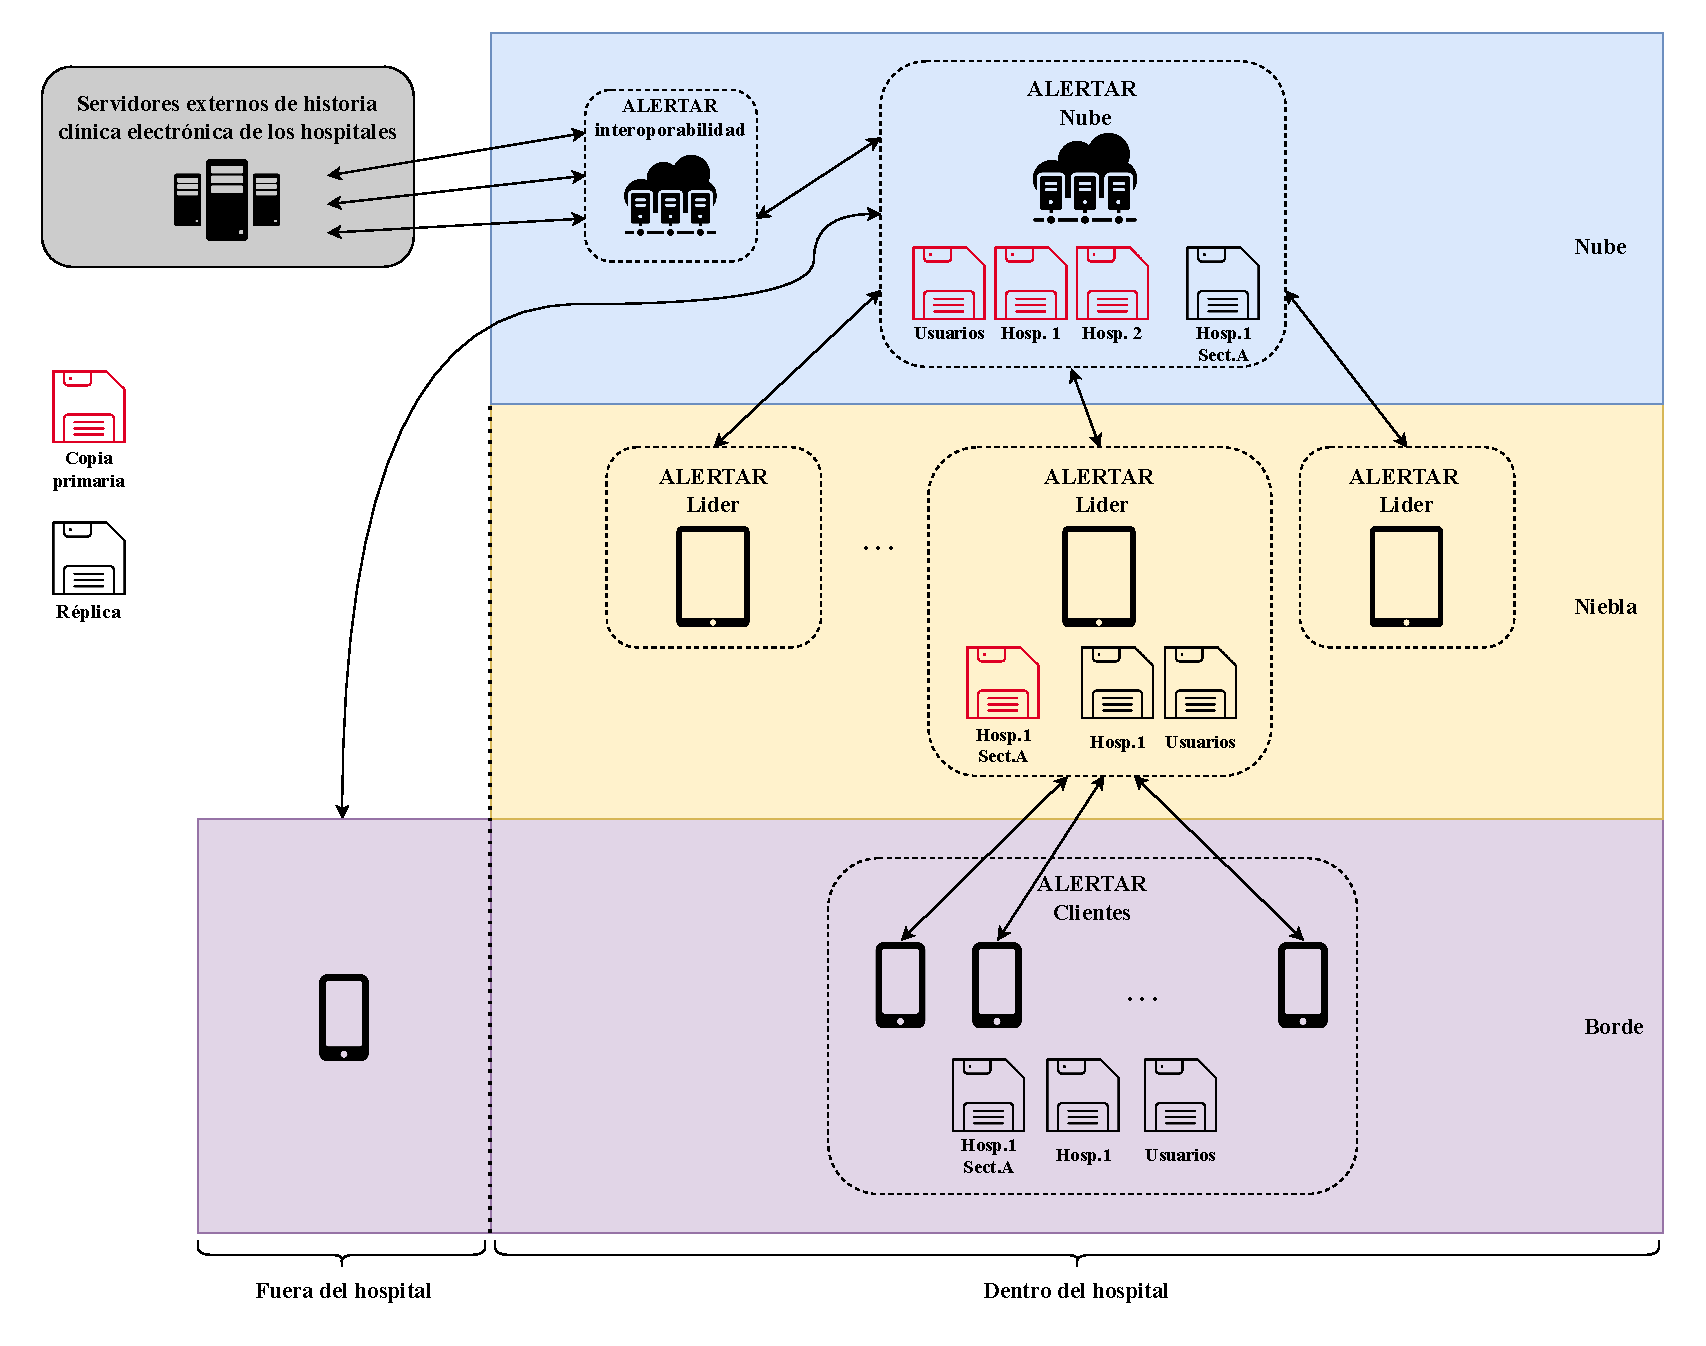
\includegraphics[width=\textwidth]{Imagenes/Arquitectura General/Componentes del sistema.pdf}
    \caption{Arquitectura de ALERTAR}
    \label{fig:arqGeneral}
\end{figure}
\textbf{Borde \textit{(Edge)}:} El término ``Dispositivo de borde'' se refiere a los dispositivos móviles empleados por el personal médico y de enfermería. Estos dispositivos posibilitan el ingreso de datos del sistema y la observación de resultados. Establecen una conexión directa con el nivel de niebla en caso de encontrarse en la misma red de área local, o con el nivel de la nube mediante Internet. Siempre priorizando la conexión con la capa de niebla.\\


\textbf{Niebla \textit{(Fog)} :} Se refiere a dispositivos móviles ubicados dentro del hospital. Estos atienden a los dispositivos de borde a través de una conexión de red de área local. La conexión a nivel niebla permite que los hospitales en entornos donde el acceso a Internet puede ser limitado, debido a restricciones de costo o a una conexión intermitente, puedan trabajar de manera efectiva y sin interrupciones.\\

\textbf{Nube \textit{(Cloud)}:} La nube mantiene una copia exhaustiva e histórica de todas las bases de datos de dispositivos a nivel de niebla. Además de ser la principal reserva de datos administrativos del hospital, almacena información compartida entre todos los hospitales. Esta capacidad de almacenamiento centralizado simplifica la gestión y el acceso a la información para todos los usuarios autorizados. Por otro lado, la conexión a nivel de la nube, actúa como nexo entre los dispositivos que se encuentren fuera de los hospitales y la capa de niebla.

%Usar orden de las diapos THAIS_2023
%Datos en reposo
\section{Organización y ubicación de los datos}
\label{sec:OrganizacionYUbicacionDatos}

El almacenamiento de datos se organiza en función de la resiliencia. Es decir que el lugar donde se almacenan los datos y de qué manera se hace, se determina en función de los servicios que tengan la capacidad de mantenerse operativos, de manera completa o parcial, ante la ocurrencia de fallos. El almacenamiento se organiza en copias primarias y réplicas. Las copias primarias son la copia original de los datos. Las réplicas son duplicados exactos utilizados para tener tolerancia a fallos.


El dominio de datos se divide en los siguientes dominios:
\begin{itemize}
    \item \textbf{Dominio de usuarios:} Contiene los datos personales del personal de salud que trabaja en los hospitales, como nombres, direcciones de correo electrónico y datos de contraseñas. Solo existe una instancia de este dominio. La nube posee la copia primaria de este dominio. Los dispositivos de niebla y borde poseen réplicas de este dominio.
    \item \textbf{Dominios de hospitales:} Comprende la información específica de cada hospital, como su nombre, dirección y otros detalles relevantes. Además, incluye datos sobre los usuarios que forman parte del personal del hospital, como su número de identificación y rol en la institución. También se encuentran registros relacionados con los diferentes sectores o áreas funcionales dentro del hospital. Cada hospital tiene su propia instancia de dominio, lo que permite una gestión detallada y personalizada de la información para cada centro médico. La nube posee la copia primaria de estos dominios. Los dispositivos de niebla y borde poseen réplicas del dominio hospital en el que se encuentran.
    \item \textbf{Dominios de sectores:} Contiene la información de cada área funcional o sector dentro del hospital. Esto incluye información de alertas médicas, datos personales y clínicos de los pacientes, información sobre la disponibilidad de camas y personal asignado al sector. Además, se registran eventos importantes como la apertura y el cierre de episodios clínicos, junto con los procesos de ingreso y egreso de pacientes. Un dispositivo de niebla es asignado para ``liderar'' a cada sector, este dispositivo es el que contiene la copia primaria del sector. El dispositivo a cargo del sector puede cambiar en cualquier momento y su reemplazo pasará a tener la copia primaria. Los dispositivos de borde poseen réplicas del dominio del sector en el que se encuentran y la nube posee réplicas de todos los dominios sector.
    
\end{itemize}
 Cada instancia de dominio es asociada con un componente del sistema, dispositivo de niebla o nube, que mantiene la copia primaria de los datos. Cuando un dispositivo desea almacenar un registro de datos para un dominio específico, debe enviar una solicitud al componente del sistema que posee la copia primaria de ese dominio. Una vez que el dato fue exitosamente almacenado en la copia primaria, se envía una copia a todos los dispositivos de borde de ese dominio, incluido el dispositivo que realizó la solicitud. 
 
 Además, el dispositivo que contiene la copia primaria de un dominio, puede procesar los nuevos registros en conjunto con los datos históricos a fin de generar nuevos registros. Por ejemplo, la inserción de un nuevo registro de paciente puede generar un nuevo registro relacionado con la clasificación de triaje.
 
 En la Figura \ref{fig:arqGeneral} se observan las copias primarias y réplicas de los tres tipos de dominios. Ante la ocurrencia de fallos, componentes del sistema que mantengan réplicas suplantarán, completa o parcialmente, la funcionalidad de los componentes que mantenían las copias primarias.

 Para permitir la sincronización de las réplicas, cada dominio cuenta con un reloj lógico que se incrementa al momento de la inserción de cada nuevo dato. Cada dato insertado va acompañado del nuevo valor del reloj.






\chapter{Implementación del núcleo de la aplicación móvil}\label{cap:implementacion}
Para la implementación del prototipo básico del núcleo básico de la aplicación móvil del sistema ALERTAR se utilizó TypeScript como lenguaje de programación y React Native como librería para el desarrollo de la aplicación sobre sistemas operativos móviles Android e iOS. Además, como sistema gestor de bases de datos se utilizó SQLite. Se utilizó una arquitectura limpia para asegurar la mantenibilidad y escalabilidad del código. Esto permitió la separación de aspectos y la implementación de principios SOLID \cite{martin2003agile}, mejorando la calidad del software.

Los desafíos de la implementación del prototipo de núcleo del sistema ALERTAR se detallan en la sección \ref{sec:desafiosImpl}. La implementación de un mecanismo de autenticación de dispositivos y cómo se garantiza la seguridad de las comunicaciones se explica en la sección \ref{sec:autentic_seguridad}. Una breve descripción del propósito de cada mensaje del protocolo de comunicación de nivel de aplicación utilizado está detallado en la sección \ref{sec:protocoloComunicacion}. La implementación de un gestor de mensajes discretos de nivel de aplicación es desarrollada en la sección \ref{sec:packageManager}. En la sección \ref{sec:perdidaConect}, se explica la definición y puesta en marcha de un mecanismo de detección de pérdida de conectividad de dispositivos. En la sección \ref{sec:serializacion} se detalla cómo es que se evitan errores de concurrencia al ejecutar operaciones relacionadas a los casos de uso. Por último, en la sección \ref{sec:implementacion} se describe la arquitectura propuesta de la aplicación, y se especifica la implementación realizada de casos de uso representativos.

\section{Desafíos de la implementación}

\label{sec:desafiosImpl}
Dada la naturaleza de la aplicación, donde se requiere que los mensajes lleguen en orden y sin errores, se elige TCP como protocolo de transporte. Además, ante la dificultad que presentan las redes de comunicaciones para establecer conexiones en el sentido del servidor hacia clientes, se decidió usar conexiones persistentes a fin de mantener canales de comunicación abiertos entre componentes del sistema.

Se requiere del establecimiento de un canal seguro de comunicación que contemple la confidencialidad, integridad y autenticidad de los datos. A causa de esto, se adoptó el protocolo TLS \textit{(Transport Layer Security)}.

La aplicación trabaja con mensajes discretos, pero al utilizar TCP se tiene un flujo de bytes. Por ello, es necesario un mecanismo que permita al receptor identificar en qué byte comienza y termina un mensaje. Inicialmente se consideró el uso de WebSocket \cite{fette2011websocket} ya que garantiza una conexión persistente, bidireccional y de baja latencia, sumado que los datos se transmiten como mensajes discretos. Además, opera sobre el protocolo TCP y hace uso de TLS para proveer seguridad de las comunicaciones. Sin embargo, se encontró una limitación en el contexto de React Native: la falta de librerías adecuadas. React Native no implementa WebSocket de manera nativa, por lo que hace uso de librerías de terceros. ALERTAR requiere que los dispositivos móviles de la capa de niebla actúen como servidores, pero ninguna de las librerías de WebSocket ofrece soporte para esta configuración. Todas las implementaciones existentes presuponen la presencia de servidores convencionales ejecutándose en computadoras dedicadas, excluyendo a dispositivos móviles.

Descartado el uso de WebSocket se optó por implementar un protocolo de discretización de mensajes sobre TLS/TCP, utilizando la librería $react\_native\_tcp\_socket$ \cite{react-native-tcp-socket}.

TLS utiliza certificados digitales para distribuir claves públicas y autenticar a las partes. En el caso de ALERTAR, los roles de cliente y servidor pueden cambiar dinámicamente, lo que impide depender de servidores fijos con certificados preestablecidos. Por esta razón, fue necesario diseñar e implementar un esquema dinámico para la distribución y validación de certificados, que permita asegurar las comunicaciones en un entorno donde los dispositivos pueden asumir distintos roles de forma flexible.

Por último, si bien el protocolo TCP define mecanismos para la detección de fallos de conexión, la librería $react\_native\_tcp\_socket$ presenta problemas para informar de manera apropiada e inmediata los fallos. Específicamente, cuando un dispositivo móvil pierde su conexión Wi-Fi o de datos móviles, la biblioteca no logra detectar la desconexión. A causa de esto, fue necesaria la implementación de un mecanismo de detección de pérdida de conectividad.

\section{Mecanismo de autenticación de dispositivos y seguridad de las comunicaciones}
\label{sec:autentic_seguridad}
En el sistema ALERTAR, los certificados son emitidos por dos entidades diferentes por un lado, una entidad certificante externa que genera y firma el certificado de la nube, y por otro lado, la nube es la encargada de la generación y firma de los certificados de los dispositivos móviles.

El proceso de manera resumida es el que se enumera a continuación y es el mismo planteado en la Figura \ref{fig:CADist}. Además es importante tener en cuenta el proceso de \textit{handshake TLS} explicado en la figura \ref{fig:handshakeTLS}.
\begin{enumerate}
    \item El dispositivo de borde envía un mensaje \textit{``hello''} a la nube.
    \item La nube responde con su certificado.
    \item El dispositivo de borde verifica que ese certificado esté firmado por alguna entidad certificante de confianza.
    \item Si el certificado es válido continúa el proceso de \textit{handshake TLS}.
\end{enumerate}

Cada dispositivo móvil tiene un único certificado. Este es otorgado por la nube en el momento en que el primer usuario que utiliza la aplicación hace un inicio de sesión. Por lo tanto, la primera vez que se realiza un inicio de sesión en cada dispositivo, es necesario que posea conexión a Internet para poder recibir su certificado desde la nube. Este certificado se entrega a través de un canal seguro entre el dispositivo de borde y la nube, lo cual evita un ataque tipo ``Hombre en el medio''. Esto se puede realizar de las siguientes dos maneras:

\begin{itemize}
    \item \textbf{Mediante un canal seguro con la nube:} Este caso se cumple una vez establecida la conexión con la nube. El dispositivo de borde al ejecutar el caso de uso \textit{datasync}, recibe desde la nube el número de \textit{IP} y certificado del dispositivo de niebla a cargo del dominio sector que se quiere conectar. Luego se desconecta de la nube e inicia una conexión al dispositivo de niebla. En caso de fracasar la conexión con el dispositivo de niebla, luego de informar al usuario del fracaso, el dispositivo de borde se vuelve a conectar a la nube.
    
    \item \textbf{Mediante código \textit{QR}:} Los dispositivos pueden tener problemas de conectividad con la nube, por esto es que tienen la posibilidad de escanear un código \textit{QR} que se muestra en la pantalla del dispositivo de niebla al que se desean conectar. Este \textit{QR} contiene el número de \textit{IP} y certificado del dispositivo de niebla para poder realizar la conexión exitosamente. Una vez obtenida esa información, el dispositivo de borde procede a intentar realizar una conexión con dicho dispositivo de niebla.
\end{itemize}

El uso de códigos \textit{QR} como medio de transmisión de certificados no garantiza la seguridad del canal de comunicación, ya que la información codificada puede ser interceptada o manipulada. No obstante, este método cumple con los requisitos de seguridad establecidos en la fase actual del proyecto, proporcionando una solución temporal y práctica para la distribución de certificados en escenarios controlados.

Haciendo uso de una estrategia de \textit{pinning} los dispositivos de borde pueden especificar una lista de certificados de confianza. En la Figura \ref{fig:distClavesALERTAR} se describe el procedimiento de generación, distribución y verificación de certificados. En esta figura se asume que se tienen dos dispositivos, uno que se convertirá en dispositivo de niebla y otro que se convertirá en dispositivo de borde. El de borde se quiere conectar al de niebla. Además, inicialmente, se establece una conexión de ambos con la nube. A continuación se describe cada uno de los pasos que se realizan desde la puesta en marcha del sistema:
\begin{enumerate}
    \item La nube obtiene un certificado generado y firmado por una entidad certificante externa.
    \item Se realiza el \textit{handshake TLS}, descrito en la Figura \ref{fig:handshakeTLS}, entre el dispositivo que será de niebla y la nube. 
    \begin{enumerate}[2.1]
        \item El futuro dispositivo de niebla valida que el certificado proporcionado por la nube durante el \textit{handshake TLS} sea válido. La validación se realiza utilizando el almacén de certificados raíz confiables del sistema operativo del dispositivo, ya que la librería empleada no incorpora su propio almacén. A pesar de esto, la librería permite especificar manualmente una autoridad certificante.
    \end{enumerate}
    \item Una vez establecido el canal seguro luego del \textit{handshake  TLS}, en caso de que sea el primer \textit{login} del futuro dispositivo de niebla, la nube le entrega un certificado que será exclusivamente utilizado por el futuro dispositivo de niebla para validar su identidad con los dispositivos de borde. Una vez recibido el certificado, el dispositivo realiza la petición para convertirse en dispositivo de niebla de un dominio \textit{sector}.
    \item El dispositivo de borde y la nube realizan el \textit{handshake TLS}.
    \begin{enumerate}[4.1]
        \item El dispositivo de borde valida que el certificado, proporcionado por la nube durante el \textit{handshake TLS}, sea válido.
    \end{enumerate}
    \item Mismo funcionamiento que el paso 3, en este caso se le entrega un certificado propio ya que ese dispositivo, que ahora es de borde, en el futuro se puede convertir a dispositivo de niebla y necesitar un certificado para identificarse con otros dispositivos de borde.
    \item El dispositivo de borde se desconecta de la nube para conectarse al dispositivo de niebla. Se realiza un \textit{handshake TLS} entre dispositivo de borde y el dispositivo de niebla, en el cual el dispositivo de niebla le entrega su certificado al de borde.
    \begin{enumerate}[6.1]
        \item El dispositivo de borde verifica en su lista de certificados de confianza si se encuentra el certificado del dispositivo de niebla, en caso de ser así este considera que es un certificado válido y el proceso de \textit{handshake TLS} finaliza con éxito. En caso de fallo, el dispositivo de borde se vuelve a conectar a la nube.
    \end{enumerate}
\end{enumerate}



\begin{figure}
    \centering
    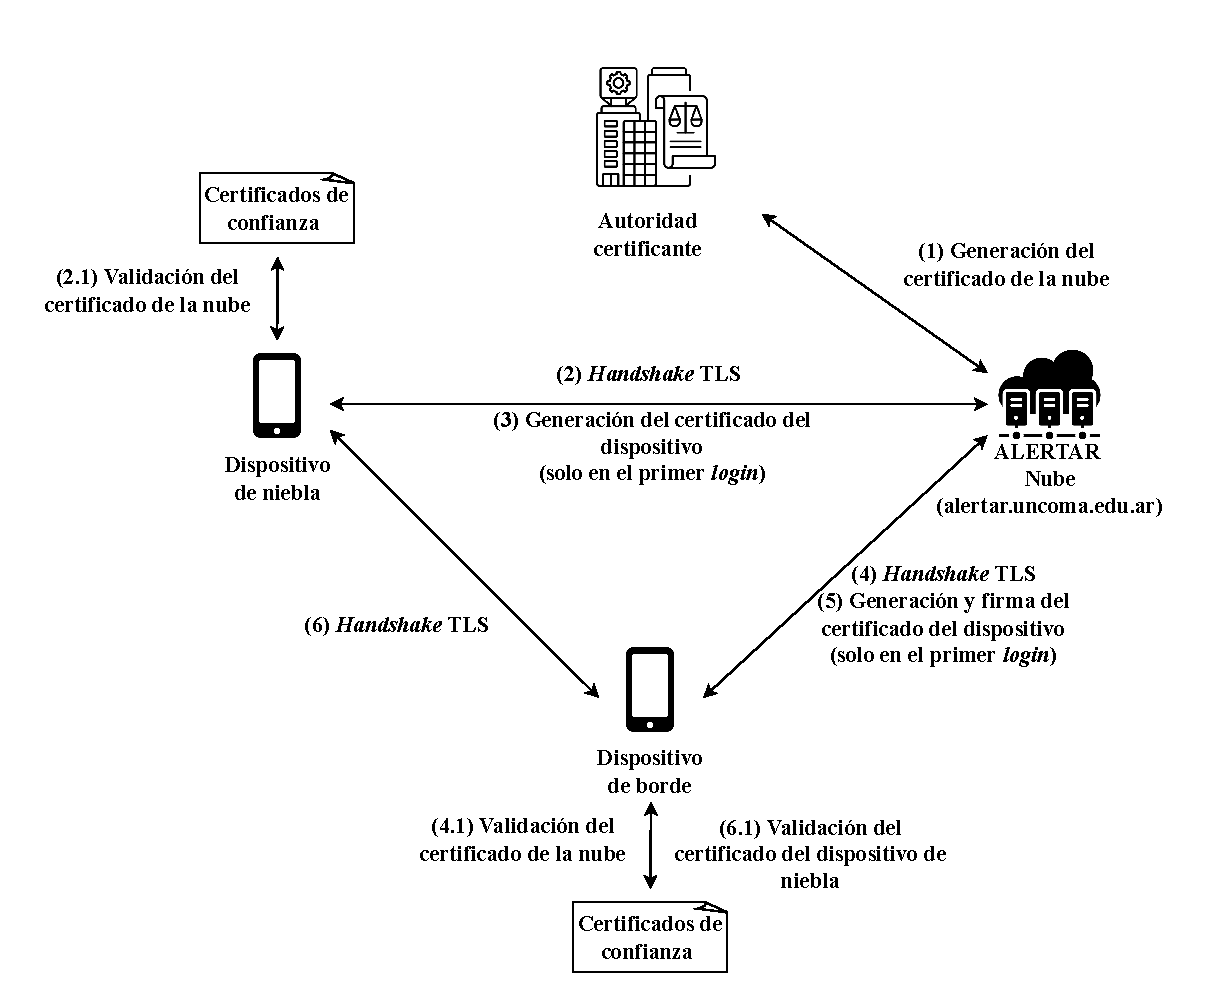
\includegraphics[width=\textwidth]{Imagenes/Implementacion/distribucionClaves.pdf}
    \caption{Generación, distribución y validación de certificados en el sistema ALERTAR}
    \label{fig:distClavesALERTAR}
\end{figure}

\section{Protocolo de comunicación}
\label{sec:protocoloComunicacion}
El sistema ALERTAR divide sus funcionalidades en casos de uso, la implementación de estos requiere del intercambio de información entre los componentes del sistema de las capas nube, niebla y de borde a través de mensajes. Con el propósito de permitir la interoperabilidad entre sistemas de cómputo heterogéneos, los mensajes se estructuran en formato JSON \cite{json_es} y se codifican utilizando el estándar UTF-8. Las operaciones se definen por el denominado \textit{protocolo de operaciones} y están definidas como:

\begin{itemize}
    \item \textit{\textbf{login: }}el usuario envía sus credenciales de identificación a un dispositivo de nivel de niebla o nube, según corresponda. Si la autenticación es exitosa, se responde con una lista de dominios (usuarios, hospitales y sectores) a los que el usuario puede suscribirse. Al finalizar, el dispositivo del usuario pasa a ser un dispositivo de borde.

    \item \textit{\textbf{data\_sync: }}luego de una autenticación exitosa, el dispositivo de borde sincroniza sus réplicas con las copias primarias de los dominios de su interés. Para esto, se envía un mensaje especificando, para cada dominio, el valor del reloj lógico más alto que tiene entre sus datos almacenados. Por cada dominio se reciben todos los datos que contengan un valor de reloj lógico mayor al especificado. Además, sólo en caso de estar sincronizado con la nube y no así con un dispositivo de niebla, se reciben los datos necesarios para establecer conexión con los dispositivos que mantienen las copias primarias de los dominios de interés. Por último, se realiza un cambio de conexión entre el dispositivo de borde y la nube, en caso de que exista, a una conexión entre el dispositivo de borde y el dispositivo de niebla a cargo del dominio de interés. Este procedimiento se detalla en la sección \ref{sec:autentic_seguridad}.

    \item \textit{\textbf{insert:}} es una petición de inserción de un nuevo dato al dispositivo que contiene la copia primaria del dominio. Verifica que no exista un registro con las mismas claves. Si la inserción es exitosa el dato se replica a través del método de \textit{copy}.

    \item \textit{\textbf{update:}} es una petición de modificación de un dato al dispositivo que contiene la copia primaria del dominio. A fin de mantener un registro histórico, la base de datos no modifica el registro original, sino que crea uno nuevo. Al insertar un nuevo registro, este tendrá un reloj lógico mayor al previo. Si existen varios registros con las mismas claves, el de mayor reloj lógico será el válido. Verifica que ya exista un registro con las mismas claves. Si la actualización es exitosa, el dato se replica a través del método \textit{copy}.

    \item \textit{\textbf{copy:}} cuando un dato es ingresado a la copia primaria, el dispositivo que la mantiene utiliza este mensaje para replicar el dato a todos los dispositivos que mantienen réplicas.


    \item \textit{\textbf{lead: }}es una solicitud a la nube para convertir dispositivos de borde en dispositivos de niebla. El usuario debe estar autorizado por la nube para realizar tal acción. Se debe especificar la dirección \textit{IP} y la clave pública del dispositivo. Esta información luego es utilizada para que los dispositivos de borde puedan intentar conectarse al de niebla a través de la red de área local.
\end{itemize}

La restricción para que funcione este protocolo es que una parte no puede enviar una nueva solicitud de operación hasta que la solicitud anterior haya sido resuelta.

En la Figura \ref{fig:secuenciaProtocolo} se detalla, a modo de ejemplo, un diagrama de secuencia donde se realiza un inicio de sesión, sincronización de datos e inserción de un nuevo paciente. Previo al inicio del ejemplo se considera que el cliente obtuvo la dirección del líder mediante un código QR o desde la nube:
\begin{enumerate}
    \item Un dispositivo de borde realiza una solicitud de \textit{login} al dispositivo de niebla a cargo del sector.
    
    \item Una vez recibida la solicitud el dispositivo de niebla prepara la respuesta \textit{infoUsuario} con información del usuario, así como los dominios a los cuales tiene permiso para suscribirse.
    
    \item Una vez recibida la respuesta al \textit{login}, el usuario procede a elegir uno o varios dominios para suscribirse. Luego se genera \textit{conjuntoDominios} el cual contiene el mayor valor de \textit{sync\_id} de cada dominio seleccionado. Finalmente, se realiza el envio en una solicitud de \textit{data\_sync} al dispositivo de niebla.

    \item Al recibir la solicitud de \textit{data\_sync}, el dispositivo de niebla, genera la respuesta \textit{datosDominios} a partir de los registros de cada dominio que tengan un \textit{sync\_id} mayor al especificado en la solicitud.

    \item El dispositivo de borde recibe los registros actualizados de sus dominios y actualiza su base de datos con estos.

    \item Al insertar un paciente, el dispositivo de borde solicita al usuario que ingrese los datos del paciente a ingresar. Una vez cargados estos datos se prepara \textit{datosPaciente} con ellos. Se envía una solicitud de inserción del paciente al dispositivo de niebla.

    \item Al recibir una solicitud de inserción el dispositivo de niebla realiza las validaciones correspondientes y, si está todo correcto, inserta un nuevo registro paciente en su base de datos local. Luego procede a realizar un proceso de \textit{copy} donde envía una solicitud con el nuevo registro a todos los dispositivos de borde suscritos al dominio que este dispositivo controla y a la nube en caso de tener conexión a ella.

    \item Todos los dispositivos de borde suscritos al dominio del sector operado, y la nube, reciben una solicitud de \textit{copy} para que guarden en su base de datos un nuevo registro
\end{enumerate}

Los pasos del uno al cinco se realizan una única vez por conexión, a la hora de establecerla. Los pasos del seis al ocho se realizan cada vez que se desea insertar un nuevo paciente.

\begin{figure}
    \centering
    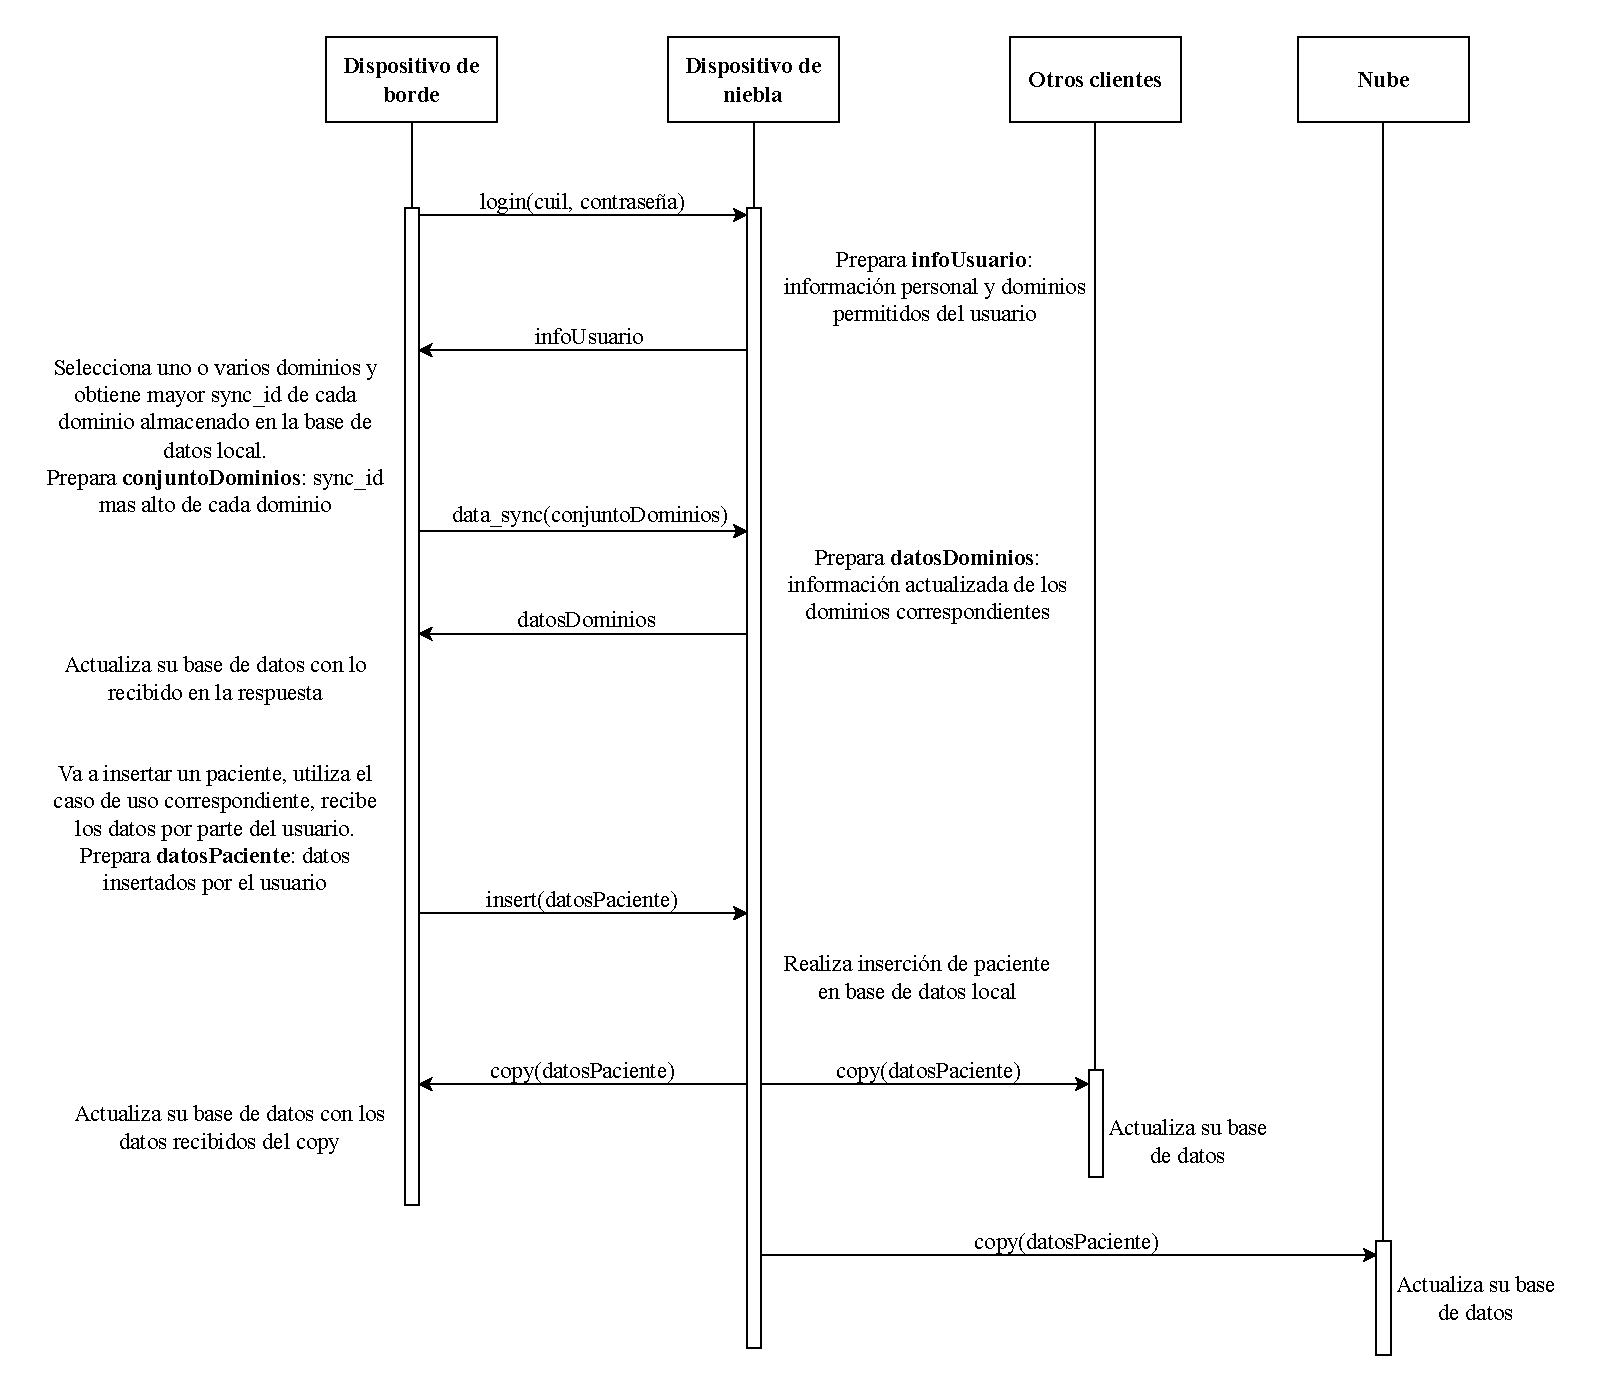
\includegraphics[width=\linewidth]{Imagenes/Implementacion/secuenciaProtocolo.pdf}
    \caption{Ejemplo de login, sincronización e inserción de paciente desde un dispositivo de borde.}
    \label{fig:secuenciaProtocolo}
\end{figure}

\section{Implementación de un manejador/gestor de mensajes discretos}
\label{sec:packageManager}
La aplicación ALERTAR requiere el envío y recepción de mensajes discretos. El protocolo TCP garantiza la entrega correcta y en orden de los datos al destinatario, pero no implementa el envío de los mensajes discretos. TCP puede particionar los mensajes en segmentos más pequeños durante la transmisión y luego re-ensamblarlos en el destino, pudiendo ocurrir que la cantidad de segmentos leídos en el destino no se corresponda con la cantidad de segmentos emitidos.

Por ejemplo, si un dispositivo de borde está conectado a un servidor y se envían los mensajes \texttt{Primer mensaje, Segundo mensaje,Tercer mensaje} de forma consecutiva, estos mensajes podrían enviarse en tres segmentos separados de la forma \texttt{[Primer mensaje], [Segundo mensaje], [Tercer mensaje]}. Alternativamente, los mensajes podrían agruparse en dos segmentos de la forma \texttt{[Primer mensajeSegun],[do mensajeTercer mensaje]}. Podrían enviarse todos juntos en un único segmento \texttt{[Primer mensaje\allowbreak Segundo mensaje\break Tercer mensaje]}. Por último, puede ocurrir que un único mensaje sea dividido en segmentos diferentes de la forma \texttt{[Pri], [me],[r mensaje]}.

Para lograr la implementación del envío de mensajes discretos se diseñó e implementó una biblioteca denominada TCP-package-manager. La biblioteca implementa un protocolo para el envío de mensajes que se define de la siguiente manera:

\paragraph{Lado del emisor:}
\begin{enumerate}
    \item Calcular la longitud del mensaje en bytes. Representar esta longitud como un entero sin signo de 4 bytes \textit{big-endian}. Por ejemplo, la longitud del mensaje \texttt{0x48 45 4C 4C 4F 20 57 4F 52 4C 44 21} se representa como \textit{0x00 00 00 0C}.
    \item Enviar la longitud calculada del mensaje.
    \item Enviar el mensaje original.
\end{enumerate}

\paragraph{Lado del receptor:}
\begin{enumerate}
    \item El receptor lee cuatro bytes del \textit{socket} de comunicaciones TLS/TCP.
    \item Interpretar los cuatro bytes leídos como la longitud del próximo mensaje, considerando que los bytes están en formato \textit{big-endian}.
    \item El receptor lee los $N$ bytes especificados en el paso anterior. Estos bytes contienen el mensaje original del emisor. En caso de que se reciba un segmento de menos de $N$ bytes se almacenan hasta que se logre completar los $N$ bytes especificados.
    
\end{enumerate}
El cálculo y envío de la longitud del mensaje original le permite al receptor saber cuántos bytes debe leer. Esto le permite leer correctamente los mensajes recibidos por más que estos no se envíen de forma discreta.

Realizando la conversión a \textit{big-endian} para el envío y su posterior interpretación en el lado del receptor, se asegura la correcta interpretación de los datos independientemente del dispositivo o arquitectura. Esto es importante ya que los procesadores pueden tener diferentes arquitecturas de \textit{endianness}, que determinan el orden en que se almacenan en memoria los bytes de datos multibyte, como enteros o flotantes.

\section{Mecanismo de detección de pérdida de conectividad}
\label{sec:perdidaConect}
Si bien el protocolo \textit{TCP} define mecanismos para la detección de fallos de conexión, la biblioteca utilizada para establecer comunicaciones \textit{TLS/TCP} presenta problemas para informarlos de manera apropiada e inmediata. Específicamente, cuando un dispositivo móvil pierde su conexión \textit{Wi-Fi} o de datos móviles, la biblioteca no logra detectar la desconexión. 

Para solucionar este problema, se implementó un protocolo de \textit{Heartbeat} y reconexión. En este protocolo, los dispositivos de borde envían un mensaje de \textit{``ping''} cada cierto tiempo. Una vez enviado el mensaje de \textit{``ping''}, los dispositivos de borde esperan una respuesta de \textit{``pong''} por parte del servidor, ya sea un dispositivo de niebla o la nube. La espera esta limitada a un tiempo $T$. Si $T$ expira, se considera que la conexión del dispositivo se ha cortado y se inicia un proceso de reconexión al líder. 

Si el servidor al que el dispositivo de borde está conectado es la nube, se consideran dos escenarios para la reconexión:

\begin{itemize}
    \item \textbf{Falla la nube: }Actualmente la nube no cuenta con reemplazo, pero cuando lo tenga se resolverá de manera transparente mediante \textit{DNS}. Los intentos de reconexión del protocolo son ilimitados. Es decir, se intentará reconectar a la nube hasta que se restablezca la conexión o se opte por conectarse manualmente a un dispositivo de niebla.
    \item \textbf{Falla la conectividad con la nube: }Los intentos de reconexión son ilimitados.
\end{itemize}

En el caso de que el servidor al que el dispositivo de borde estaba conectado se trate del dispositivo de niebla, como el problema de conexión puede deberse a un fallo del servidor, y el reemplazo no es transparente, luego de un determinado número de intentos se considera que la conexión se ha perdido de forma definitiva. En este caso, la aplicación inicia nuevamente la conexión al sistema, que comienza estableciendo contacto con la nube.

\begin{figure}
    \centering
    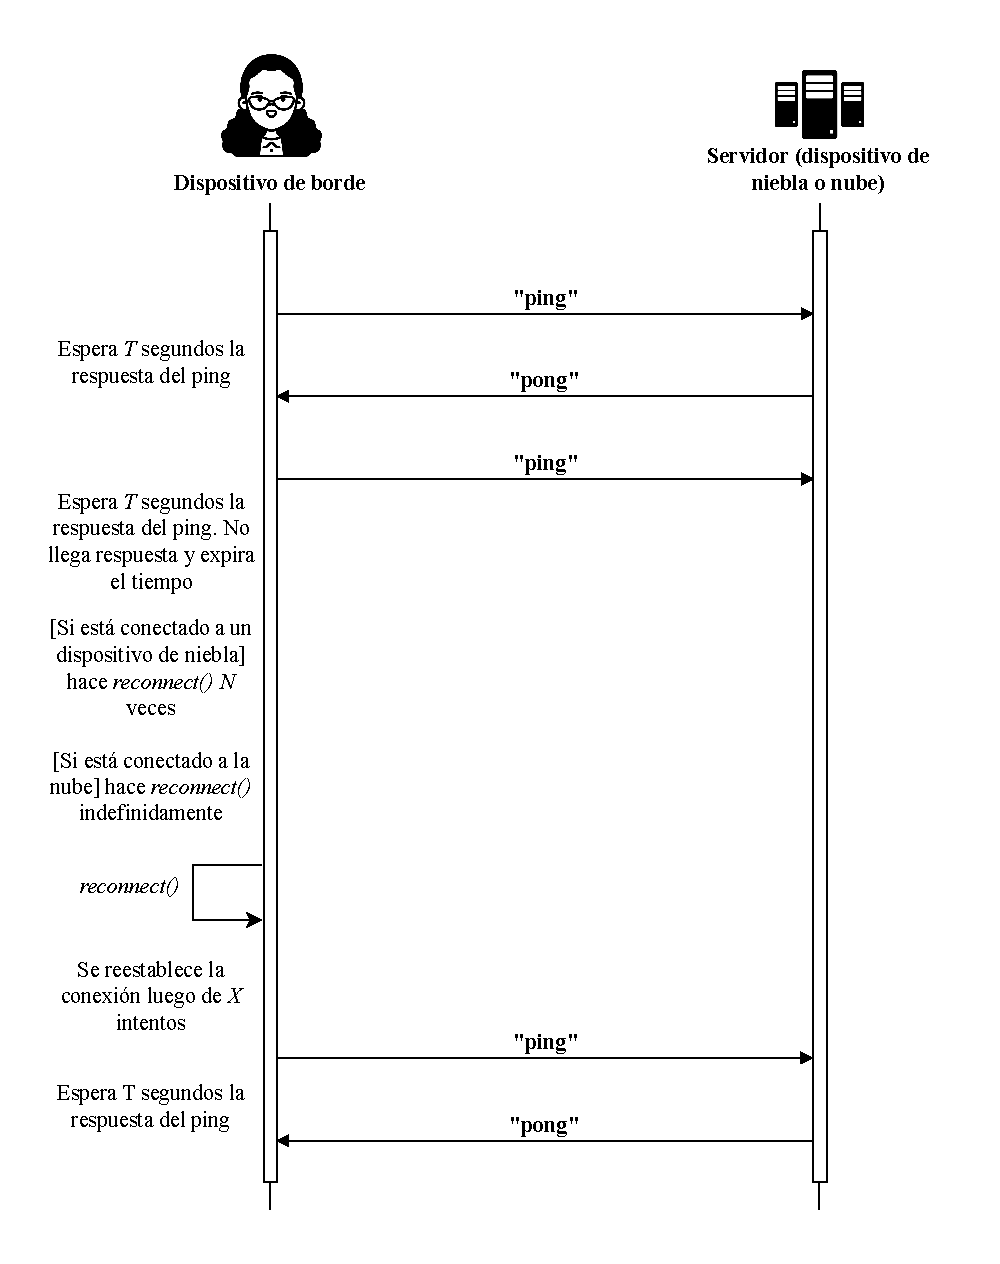
\includegraphics[width=14cm]{Imagenes/Implementacion/ProtocoloReconexion.pdf}
    \caption{Funcionamiento del protocolo de \textit{Ping} y reconexión ante fallos}
    \label{fig:protocoloReconexion}
\end{figure}


Al implementar este protocolo, los usuarios no deben preocuparse por la reconexión manual de los dispositivos, ya que el sistema se encarga automáticamente de detectar desconexiones y de restablecer la conexión ya existente sin necesidad de intervención del usuario. En caso de que no haya conectividad con la nube y el usuario desee cambiar la conexión a un nuevo dispositivo de niebla que se encuentre operativo, el proceso de conexión deberá realizarse de manera manual haciendo uso de un código \textit{QR} que se muestra en la pantalla del dispositivo de niebla al que se desea conectar.

En la figura \ref{fig:protocoloReconexion} se puede observar un ejemplo de su funcionamiento. En ella se asume que ya hay establecida una conexión previa entre un dispositivo de borde y un servidor nube o dispositivo de niebla. Se puede observar el intercambio de mensajes \textit{``ping''} y \textit{``pong''} entre las partes, cada vez que el dispositivo de borde envía un mensaje de \textit{``ping''} espera un tiempo $T$ a que el servidor le responda con un \textit{``pong''}. En caso de que el tiempo $T$ expire se considera que hubo una pérdida de conexión, en cuyo caso se plantean dos posibles escenarios:
\begin{itemize}
    \item El dispositivo de borde está conectado a un dispositivo de niebla: Se procede a realizar los $N$ intentos de reconexión haciendo uso de \textit{reconnect()}.
    \item El dispositivo de borde está conectado a la nube: Se procede a realizar intentos de reconexión de manera indefinida con \textit{reconnect()}.
\end{itemize}

Una vez restablecida la conexión se reanuda el intercambio de mensajes entre las partes.





\section{Serialización de las operaciones}
\label{sec:serializacion}
Para evitar la aparición de errores o estados inconsistentes en los dispositivos y mantener la consistencia del sistema, es crucial garantizar que las operaciones sean procesadas en el mismo orden en el que son recibidos los mensajes que las accionan.

Para comprender qué ocurre ante la inexistencia de serialización, se plantea el siguiente escenario como ejemplo: un dispositivo de borde recibe dos peticiones de \textit{copy} por parte del dispositivo de niebla. La primera tiene un registro paciente con $sync\_id=4$ y la segunda un registro paciente $sync\_id=5$. Se asume que las operaciones en el dispositivo de borde no están serializadas. El guardado del registro con $sync\_id=5$ finaliza antes que el del registro con $sync\_id=4$. Si el dispositivo llegara a tener un fallo que impidiera finalizar la inserción del registro con $sync\_id=4$, al realizar el proceso de \textit{data\_sync} se enviará el valor de $sync\_id=5$, ya que es el más alto del dominio sector en la base de datos local del dispositivo de borde. Esto produce que el registro con $sync\_id=4$ no se vuelva a sincronizar nunca lo cual provoca la pérdida de dicho dato en la réplica del dominio sector del dispositivo de borde.

\textit{TypeScrypt} es un sistema basado en eventos con un único hilo. Para gestionar y coordinar las operaciones asíncronas, de manera que puedan ejecutarse de manera eficiente sin bloquear el hilo principal, \textit{TypeScrypt} usa el denominado \textit{event loop}\cite{ecma262}. En este, si por ejemplo, se tienen tres funciones asíncronas: \textit{validate()}, \textit{updateDataSync()}, e \textit{insert()}, y no se utiliza un mecanismo de sincronización, las funciones pueden empezar a ser ejecutadas sin esperar a que las tareas previas terminen.

Para controlar el orden de ejecución de las llamadas, TypeScript utiliza dos estructuras principales: la pila de ejecución y la cola de tareas. La pila de ejecución \textit{(stack)} es una estructura que gestiona la ejecución de funciones según el orden en que se llaman. Cuando una función es invocada, se añade a la pila y comienza su ejecución pausando la ejecución de su llamador. Si esa función llama a otra, esta nueva función también se añade a la pila y se continúa con la ejecución de esta, pausando la ejecución de la llamadora, así sucesivamente. Una vez que una función completa su ejecución, se elimina de la pila, y el control vuelve a la función anterior. Este proceso continúa hasta que la pila esté vacía, permitiendo que siga un flujo de ejecución organizado permitiendo invocaciones anidadas y recursión.

Por otro lado, al utilizar funciones asíncronas, se lanzan tareas no bloqueantes, las cuales no necesariamente son aquellas delegadas a componentes externos del sistema, que se colocan en una cola de tareas. El \textit{event loop} se encarga de gestionar estas tareas, ejecutándose cuando la pila de ejecución está vacía.

Entonces, volviendo al ejemplo donde se ejecutan \textit{validate()}, \textit{updateDataSync()}, e \textit{insert()}, cuando cualquiera de estas funciones llegue a una operación asíncrona (como una promesa\footnote{Una promesa es un objeto que representa la eventual resolución o rechazo de una operación asíncrona, permitiendo manejar su resultado en el futuro a través de métodos como \textit{.then()} o \textit{await}.} o una operación de entrada/salida (I/O)), esa tarea, que corresponde a la ejecución de la operación, se envía a la cola de tareas (En realidad TypeScript cuenta con dos colas, una de microtareas y otra de macro tareas). No se bloquea la ejecución esperando el resultado de la tarea, simplemente se continúa con la ejecución de la siguiente línea de código que corresponda. Luego, el \textit{event loop} revisa la cola de tareas y las ejecuta cuando la pila de llamadas esté vacía.

Al aplicar el mecanismo de sincronización mediante await, la pila de llamadas se detiene temporalmente en esa línea de código, esperando a que la promesa se resuelva. Una vez que la promesa se resuelve, la ejecución de la función continúa, y finalmente, cuando termina, la función se retira de la pila de llamadas. De esta manera, se garantiza la serialización de las operaciones asíncronas, ya que estas se van a ejecutar de manera secuencial y en el orden definido por el programa.

En la Figura \ref{fig:ejemploEventLoop} se puede observar un ejemplo, asumiendo que las funciones están dentro de un método \textit{main()} que se muestra en la Figura \ref{fig:eventLoopCodigo}. En la mitad izquierda de la sub figura \ref{fig:eventLoop}, la cual representa las llamadas sin el mecanismo de sincronización await, se tendrá el siguiente comportamiento:

\begin{enumerate} 
    \item \textbf{Llamada a \textit{main()}} $\rightarrow$ main() sube a la pila de llamadas.
    
    \item \textbf{Llamada a validate()} $\rightarrow$ validate() sube a la pila de llamadas. Se crea una promesa que se retorna inmediatamente y la tarea relacionada a esa promesa se envía a la cola de tareas. 
    
    \item \textbf{validate() termina} $\rightarrow$ La parte síncrona de validate() se ejecuta, y luego validate() sale de la pila de llamadas. 
    
    \item \textbf{Llamada a updateDataSync()} $\rightarrow$ updateDataSync() sube a la pila de llamadas. Se crea una promesa que se retorna inmediatamente y su resolución se guarda en la cola de tareas. 
    
    \item \textbf{updateDataSync() termina} $\rightarrow$ La parte síncrona de updateDataSync() se ejecuta, y luego updateDataSync() sale de la pila de llamadas. 
    
    \item \textbf{Llamada a insertPaciente()} $\rightarrow$ insertPaciente() sube a la pila de llamadas. Se crea una promesa que se retorna inmediatamente y la tarea correspondiente se encola para su posterior ejecución.

 \item \textbf{insertPaciente() termina} $\rightarrow$ La parte síncrona de insertPaciente() se ejecuta, y luego insertPaciente() sale de la pila de llamadas. 
    
    \item \textbf{El \textit{event loop} gestiona la cola de tareas} $\rightarrow$ Después de que la pila de llamadas esté vacía, el \textit{event} loop procesa las promesas pendientes de resolución en la cola de tareas. 
\end{enumerate}

En este caso el llamador no espera la finalización de las funciones asíncronas para continuar con su ejecución. Es decir, no se aplica ningún mecanismo de sincronización.

Para la segunda parte de la Figura \ref{fig:eventLoop}, donde sí se hace uso de \textit{await}, el método de sincronización hace una espera para que finalice cada llamada antes de continuar con la ejecución que se encuentra después de ella:

\begin{enumerate}
    \item \textbf{Llamada a \textit{main()}} $\rightarrow$ \textit{main()} sube a la pila de llamadas. Se ejecuta hasta el primer \textit{await}.
    
    \item \textbf{\textit{await validate()}} $\rightarrow$ \textit{main()} se pausa en \textit{validate()} hasta que la promesa se resuelva en la cola de tareas.
    
    \item \textbf{Resolución de \textit{validate()}} $\rightarrow$ La promesa de \textit{validate()} se resuelve, \textit{main()} se reanuda y continúa con \textit{updateDataSync()}.
    
    \item \textbf{\textit{await updateDataSync()}} $\rightarrow$ \textit{main()} se pausa en \textit{updateDataSync()} hasta que la promesa se resuelva en la cola de tareas.
    
    \item \textbf{Resolución de \textit{updateDataSync()}} $\rightarrow$ La promesa de \textit{updateDataSync()} se resuelve, \textit{main()} se reanuda y continúa con \textit{insertPaciente()}.
    
    \item \textbf{\textit{await insertPaciente()}} $\rightarrow$ \textit{main()} se pausa en \textit{insertPaciente()} hasta que la promesa se resuelva en la cola de tareas.
    
    \item \textbf{Resolución de \textit{insertPaciente()}} $\rightarrow$ La promesa de \textit{insertPaciente()} se resuelve, \textit{main()} se reanuda y finalmente termina, saliendo de la pila de llamadas.
\end{enumerate}

De esta manera, al utilizar \textit{await} en cada función asíncrona, el event \textit{loop} se encarga de pausar la ejecución de \textit{main()} hasta que cada promesa se resuelva. Esto asegura que las operaciones se ejecuten de forma secuencial, respetando el orden de las llamadas. Gracias al \textit{await}, se garantiza la ejecución secuencial de las operaciones.

\begin{figure}[]
    \centering    
    \begin{subfigure}{\textwidth}
        \centering 
        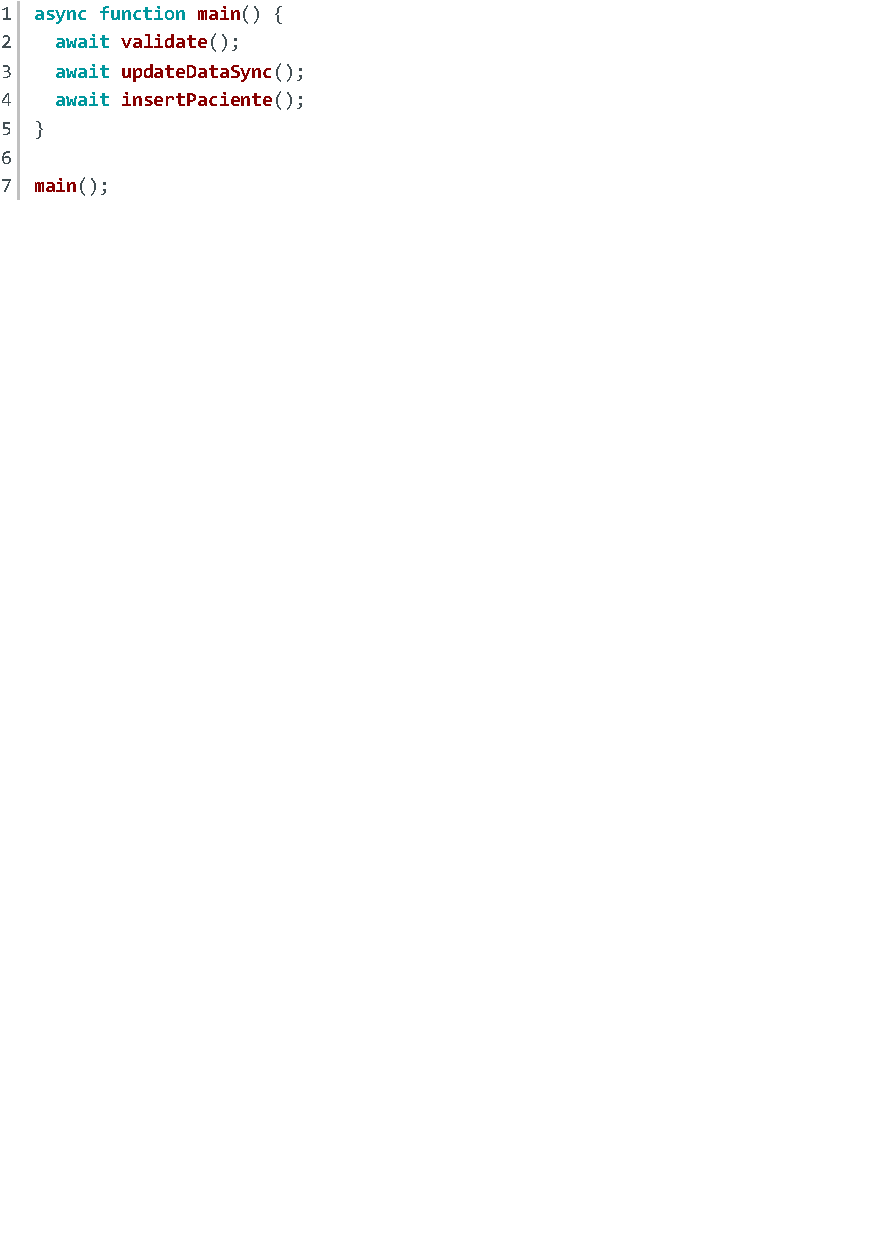
\includegraphics[width=0.5\textwidth]{Imagenes/Implementacion/eventLoopCodigo.pdf}
        \caption{Función main() contiene a las tres funciones}
        \label{fig:eventLoopCodigo}
    \end{subfigure}
    \begin{subfigure}{\textwidth}
        \centering 
        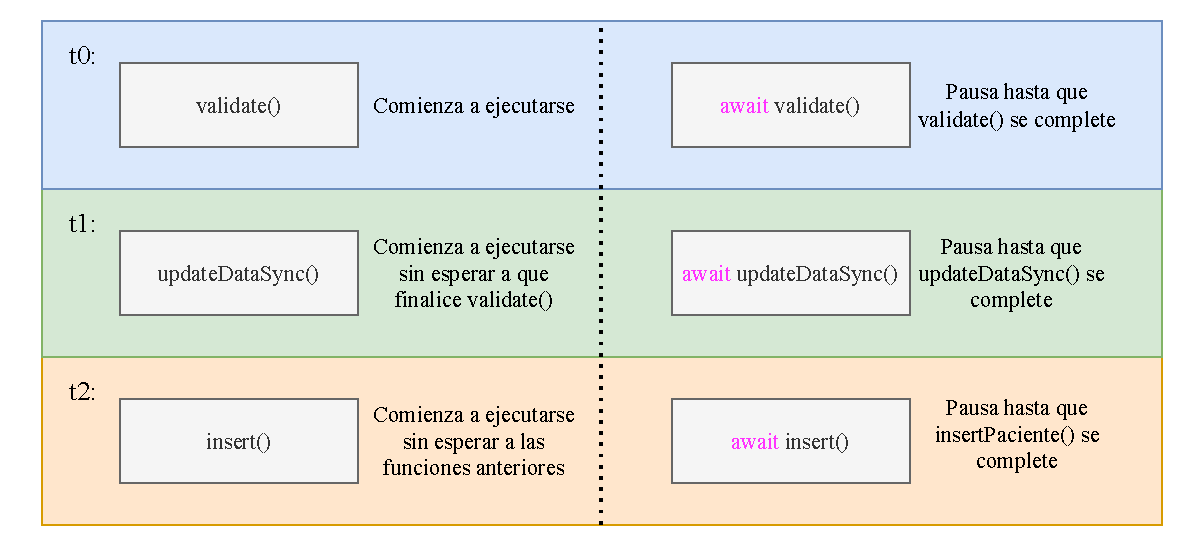
\includegraphics[width=\textwidth]{Imagenes/Implementacion/eventLoop.pdf}
        \caption{Secuencia y tiempos de llamadas del event loop}
        \label{fig:eventLoop}
    \end{subfigure}
    \caption{Ejemplo de comportamiento de event loop}
    \label{fig:ejemploEventLoop}
\end{figure}

\section{Diseño arquitectónico y especificaciones de la implementación}
\label{sec:implementacion}
La implementación del núcleo del sistema ALERTAR consiste en dos aspectos clave, los casos de uso y los servicios para los dispositivos de borde y niebla. Ambos aspectos fueron diseñados e implementados haciendo uso de una arquitectura limpia.

\subsection{Implementación de la arquitectura limpia}
Se implementaron tres capas que constituyen la arquitectura limpia del núcleo de la aplicación móvil ALERTAR. Estas se encuentran detalladas en la Figura \ref{fig:capasArquitectura} donde se puede observar, representadas con flechas, las dependencias de las capas de \textit{interfaz de usuario} y \textit{datos} con la capa de \textit{dominio}. De esta manera, se logra que los componentes de la capa de dominio sean independientes de implementaciones concretas de interfaces gráficas, bases de datos, servicios y repositorios. Las capas se definen de la siguiente manera:

\begin{itemize}
    \item \textbf{Interfaz de usuario: }Aquí se definen las interfaces a través de las cuales los usuarios interactúan con el sistema, en este caso las vistas y componentes interactivos de la aplicación móvil.
    
    \item \textbf{Dominio: }Aquí se definen los \textit{casos de uso} los cuales determinan las funcionalidades a las cuales pueden acceder los usuarios. Las \textit{entidades}, las cuales son objetos que contienen datos junto con las funciones que los manipulan, son independientes de cualquier infraestructura por lo que pueden ser utilizadas por cualquier capa de la aplicación. Por último, las \textit{interfaces de repositorios} que determinan cómo es que interactúa la capa de dominio con la capa de datos. Estas interfaces garantizan que la capa de dominio permanezca aislada e independiente de implementaciones específicas, las cuales son delegadas a la capa de datos.

    \item \textbf{Datos: }Aquí se realizan las implementaciones de los repositorios, se definen las interfaces de bases de datos y servicios, junto con sus implementaciones concretas.
\end{itemize}

\begin{figure}
    \centering
    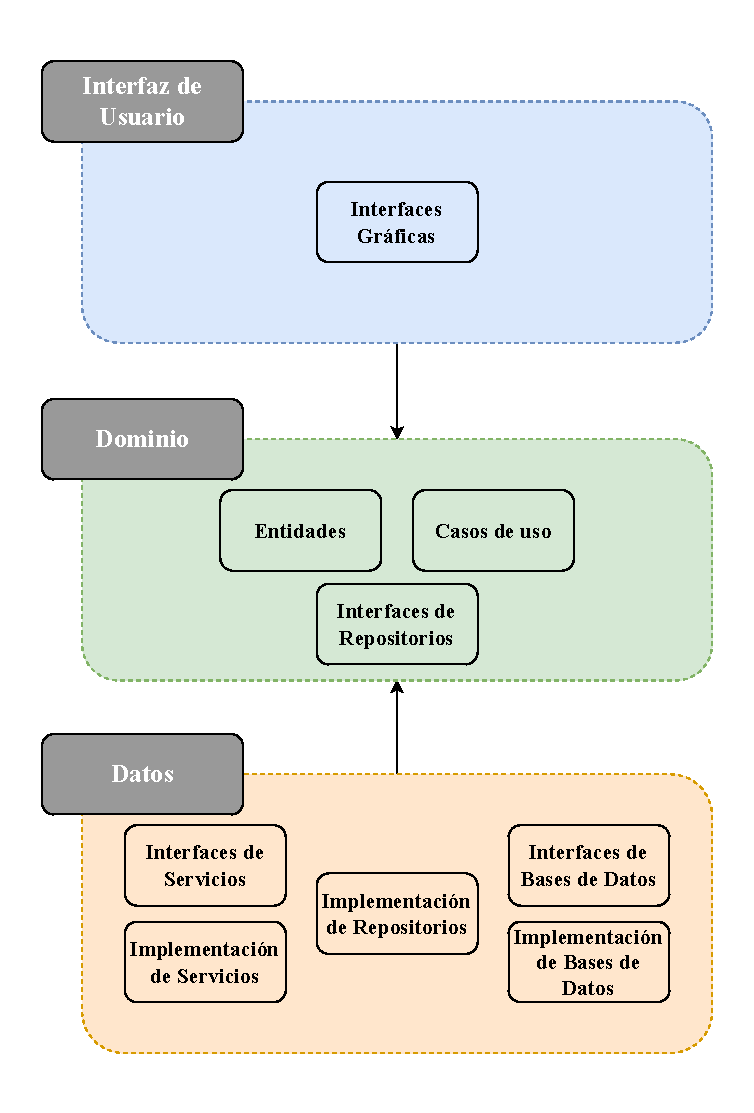
\includegraphics[width=0.7\linewidth]{Imagenes/Implementacion/CapasArquitectura.pdf}
    \caption{Arquitectura limpia del núcleo de la aplicación móvil del sistema ALERTAR}
    \label{fig:capasArquitectura}
\end{figure}
La forma en la cual interactúan entre sí las diferentes capas de la arquitectura limpia implementada se representa en la Figura \ref{fig:comunCapasArquitectura}. En ésta, los usuarios ejecutan casos de uso a través de una interfaz gráfica correspondiente a la capa de \textit{interfaz de usuario}. Los casos de uso, correspondientes a la capa de \textit{dominio}, utilizan interfaces de repositorios y entidades para definir su funcionalidad. Las implementaciones de las interfaces de los repositorios se envían a través del constructor del caso de uso. Las implementaciones de los repositorios corresponden a la capa de \textit{datos}. Por último, las clases concretas que implementan los repositorios utilizan interfaces de bases de datos y servicios, lo que las hace independientes de sus implementaciones específicas. Por ejemplo, si se quisiera cambiar el tipo de base de datos de relacional a no relacional, no sería necesario modificar la lógica del repositorio, ya que utiliza una interfaz para acceder a su fuente de datos, en lugar de depender de una implementación específica.

Además, se observa que los servicios interactúan directamente con los casos de uso, dado que las solicitudes realizadas por los dispositivos de borde hacia los de niebla requieren ser resueltas mediante la ejecución de dichos casos de uso. La recepción y cómputo de los mensajes se realiza a través de los servicios, lo que implica que estos deben invocar los casos de uso correspondientes para procesar y responder adecuadamente a las peticiones recibidas.
\begin{figure}
    \centering
    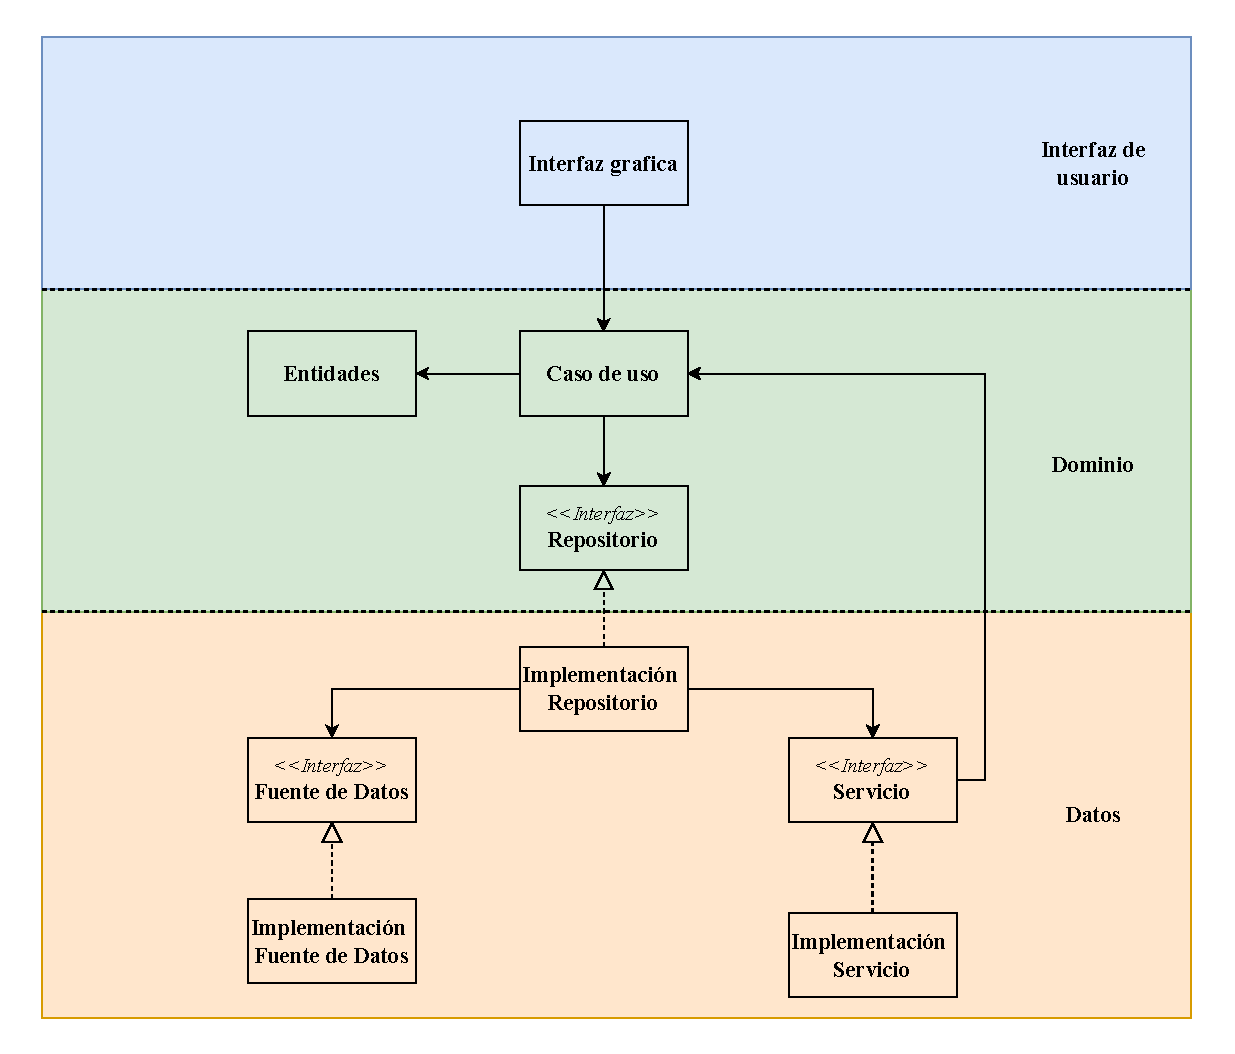
\includegraphics[width=1\linewidth]{Imagenes/Implementacion/ComunicacionCapas.pdf}
    \caption{Comunicación entre las capas de la arquitectura limpia}
    \label{fig:comunCapasArquitectura}
\end{figure}

Aplicando esta arquitectura se logra que los diferentes componentes de la aplicación puedan evolucionar o ser modificados de manera independiente. Lo que permite que el sistema sea modular, mantenible y flexible.

\subsection{Servicios de los dispositivos de borde y niebla}
Dado que los dispositivos de niebla deben actuar como servidores, se definió una interfaz denominada \texttt{LiderService}, que agrupa todas las operaciones necesarias para su gestión. Esta interfaz se ilustra en la Figura \ref{fig:liderService} y define cómo debe crearse el servidor en los dispositivos, delegando la responsabilidad a la clase \texttt{Server}. Para abstraer el tipo de protocolo de transporte utilizado, se adoptó el patrón \textit{Factory} mediante la interfaz \texttt{ConnectionFactory}, lo que permite implementar e instanciar diferentes tipos de conexión para el servidor en caso de ser necesario.


Entre las operaciones que define \texttt{LiderService} se incluyen: la creación del servidor, el manejo de nuevas conexiones, el envío de réplicas a todos los dispositivos conectados (\textit{copy}) y la recepción de mensajes discretos. Para estas últimas dos tareas, se hace uso de la clase \texttt{PackageManager}.

Una vez decodificado un mensaje por parte de un dispositivo de niebla, se determina y ejecuta el caso de uso correspondiente. Esta dependencia hacia los casos de uso se representa de manera simplificada en la Figura \ref{fig:liderService} con la clase \texttt{CasosDeUso}, la cual representa a todos los casos de uso. La clase \texttt{LiderServiceImpl}, que implementa la interfaz \texttt{LiderService}, es responsable de procesar la petición, enviar la respuesta al dispositivo de borde que la originó y propagar el \textit{copy} resultante tanto a la nube como al resto de los dispositivos de borde conectados.




\begin{figure}
    \centering
    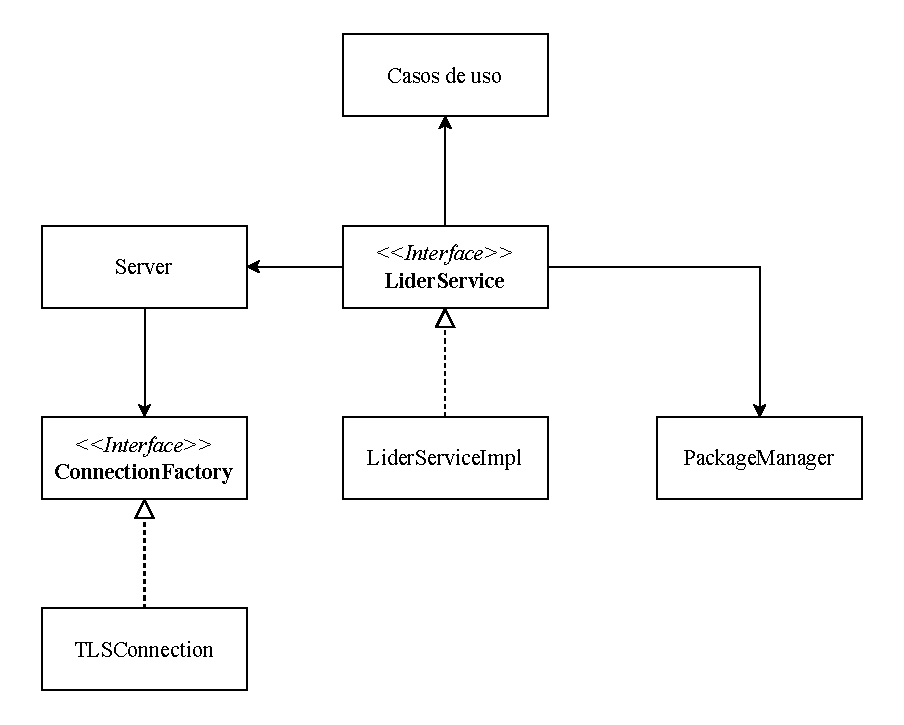
\includegraphics[width=\linewidth]{Imagenes/Implementacion/LiderService.pdf}
    \caption{Servicio de los dispositivos de niebla}
    \label{fig:liderService}
\end{figure}

Por otro lado, todos los dispositivos de borde deben conectarse a un servidor, ya sea la nube o un dispositivo de niebla. Para esto, se definió una interfaz denominada \texttt{UserService}, ilustrada en la Figura \ref{fig:clientService}. Esta interfaz, agrupa las operaciones necesarias para establecer y mantener la conexión de los dispositivos con el servidor, incluyendo: conexión, desconexión, reconexión y el envío y recepción de mensajes con el servidor. Al igual que \texttt{LiderService}, los detalles de la gestión de conexión, como por ejemplo la creación y manejo de \textit{sockets} con el servidor, se delega en la clase \texttt{Server}.

Tal como se observa en la figura \ref{fig:clientService}, \texttt{UserService} hace uso de la clase \texttt{PackageManager} para garantizar que los mensajes se transmitan como unidades discretas. La clase \texttt{PingService} es responsable de implementar el protocolo de \textit{heartbeat}, utilizado para detectar interrupciones en la conectividad y disparar los mecanismos de reconexión cuando sea necesario. Además, se necesita poder ejecutar el caso de uso de inicio de sesión para poder gestionar reconexiones de manera completa. Para esto, utiliza la clase \texttt{UserLoginUseCase}.


Por último, se debe considerar que, como todos los dispositivos se conectan al servidor a través de \texttt{UserService}. De este modo, todos los mensajes provenientes del servidor son procesados por esta clase. En caso de que un mensaje recibido requiera funcionalidad específica del rol de niebla del dispositivo, entonces \texttt{UserService} delega el manejo de dicha funcionalidad a \texttt{LiderService}.


\begin{figure}
    \centering
    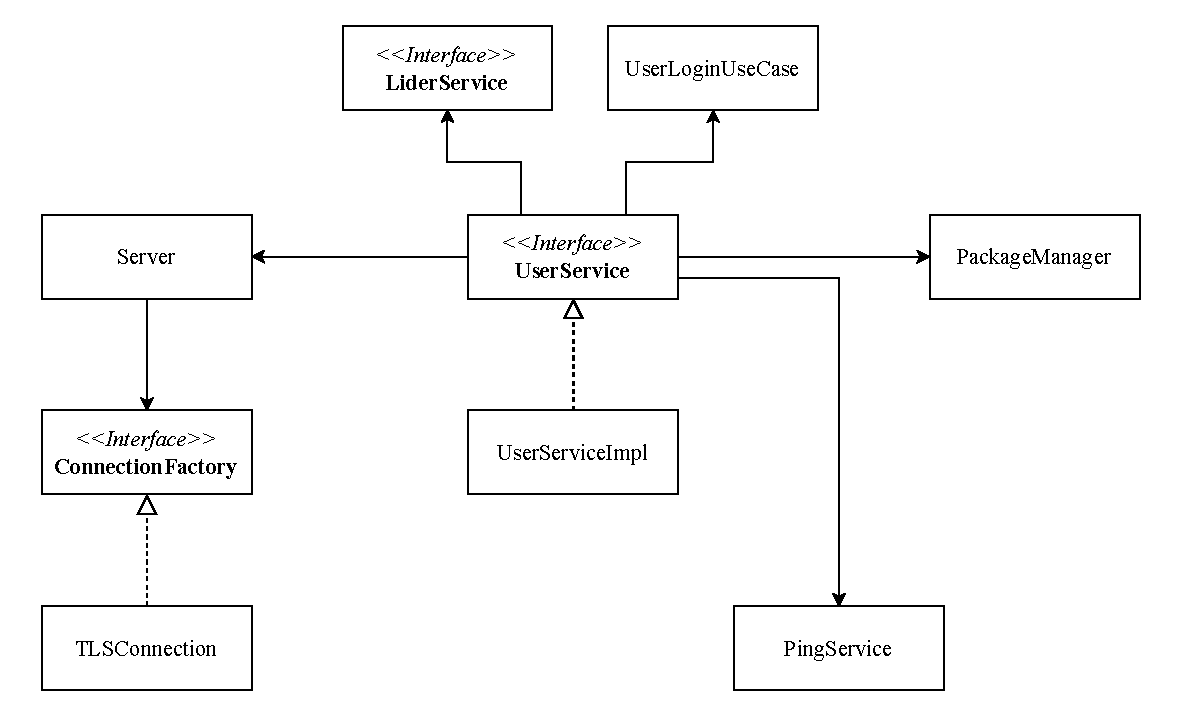
\includegraphics[width=\linewidth]{Imagenes/Implementacion/UserService.pdf}
    \caption{Servicio de los dispositivos de borde}
    \label{fig:clientService}
\end{figure}

\subsection{Casos de uso}
Los casos de uso son aquellas funcionalidades a las cuales el personal del hospital tiene acceso a través de la aplicación móvil, estan representados en el diagrama de la Figura \ref{fig:diagCasosUso} donde las flechas indican una dependencia unidireccional entre las capas. A continuación se detalla el objetivo de cada caso de uso:

\begin{itemize}
    \item \textbf{Iniciar sesión: }Valida el CUIL y contraseña del usuario para poder comenzar a utilizar la aplicación móvil. Como respuesta devuelve la información del usuario y los dominios a los cuales puede conectarse.
    \item \textbf{Conectarse a dominio:} El usuario selecciona el dominio al cual desea conectarse, como resultado se sincroniza toda la información de dicho dominio en el dispositivo móvil del usuario.
    \item \textbf{Admisión de paciente:} El usuario carga la información del paciente al ingresar. Esta operación es enviada a través de una solicitud y computada por un dispositivo de niebla. Finalmente, el dispositivo de borde del usuario, recibe una réplica por parte del dispositivo de niebla. La actualización de los pacientes es una variante de este mismo caso de uso.
    \item \textbf{Convertir a dispositivo de niebla:} El usuario convierte su dispositivo de borde a uno de niebla. Para poder hacerlo el usuario debe ser de tipo ``Jefe de enfermería'' o ``Jefe de clínica médica''
    \item \textbf{Asignar cama: }El usuario asigna un nuevo estado para una cama, es decir indica si se encuentra ocupada, desocupada o inhabilitada.
    \item \textbf{Modificar datos personales paciente: }Modifica los datos personales de un paciente ya ingresado.
    \item \textbf{Ver ficha de paciente: }Muestra la lista de fichas de todos los pacientes ingresados, permitiendo buscar una en especifico y leerla en detalle. 
    \item \textbf{Ver estado camas: }Muestra el estado de todas las camas del dominio seleccionado.
\end{itemize}

\begin{figure}
    \centering
    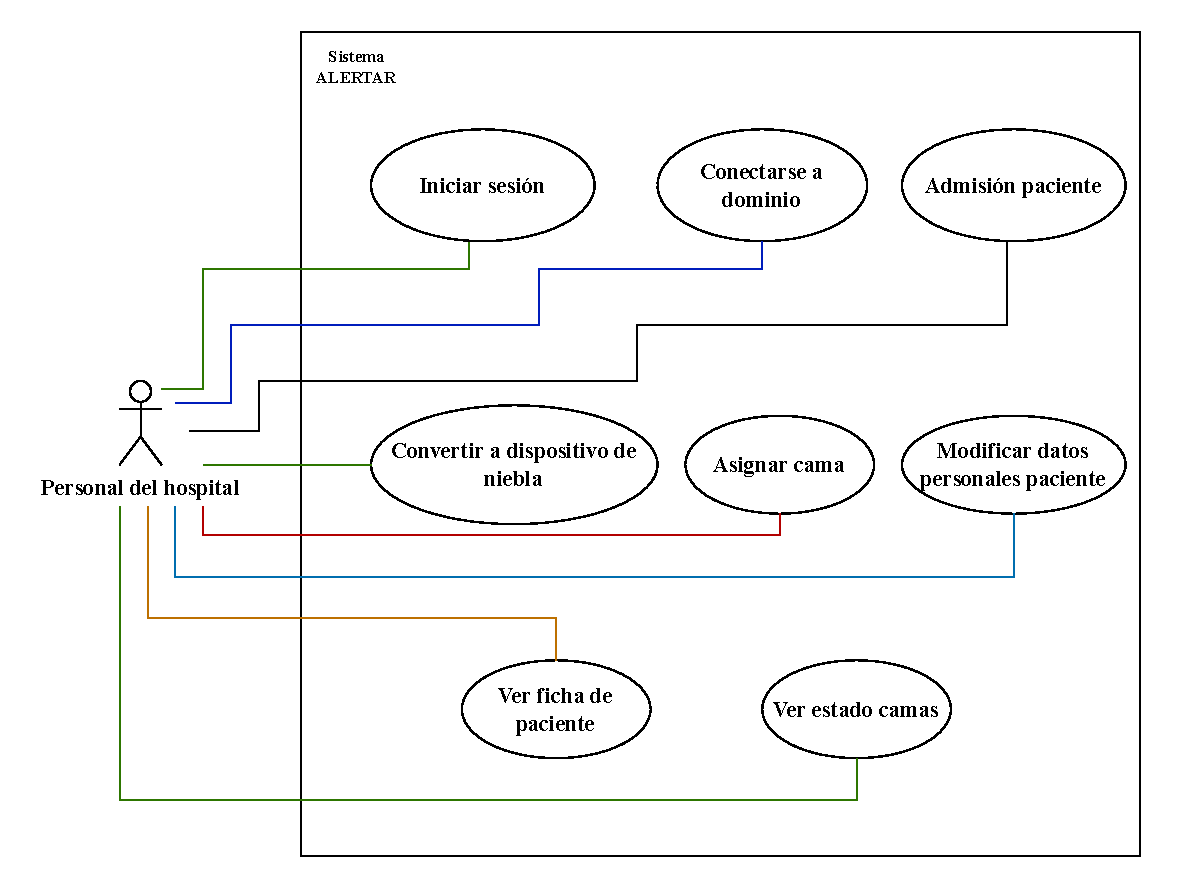
\includegraphics[width=\textwidth,keepaspectratio]{Imagenes/Implementacion/CasosDeUso.pdf}
    \caption{Diagrama de casos de uso de la aplicación móvil ALERTAR}
    \label{fig:diagCasosUso}
\end{figure}


Un diagrama de actividades del caso de uso \textit{Admisión paciente} se detalla en la Figura \ref{fig:diagActAdmPaciente}. En esta, se puede observar cómo cada conjunto de actividades se corresponde a una capa de la arquitectura limpia diseñada. El ingreso de los datos de un paciente y las notificaciones de fallo y éxito se corresponden a la capa de \textit{Interfaz de usuario}, enmarcadas en azul. La generación de la petición para computar el caso de uso, por parte del dispositivo de borde, y la validación de los datos de esta por parte del dispositivo de niebla se corresponden a la capa de \textit{Dominio}, encuadradas en verde. Por último, la creación y almacenamiento de un nuevo registro ``Paciente'' en ambos dispositivos, y la réplica del registro por parte del dispositivo de borde, corresponden a la capa de \textit{Datos}, enmarcada en amarillo.

\begin{figure}
    \centering
    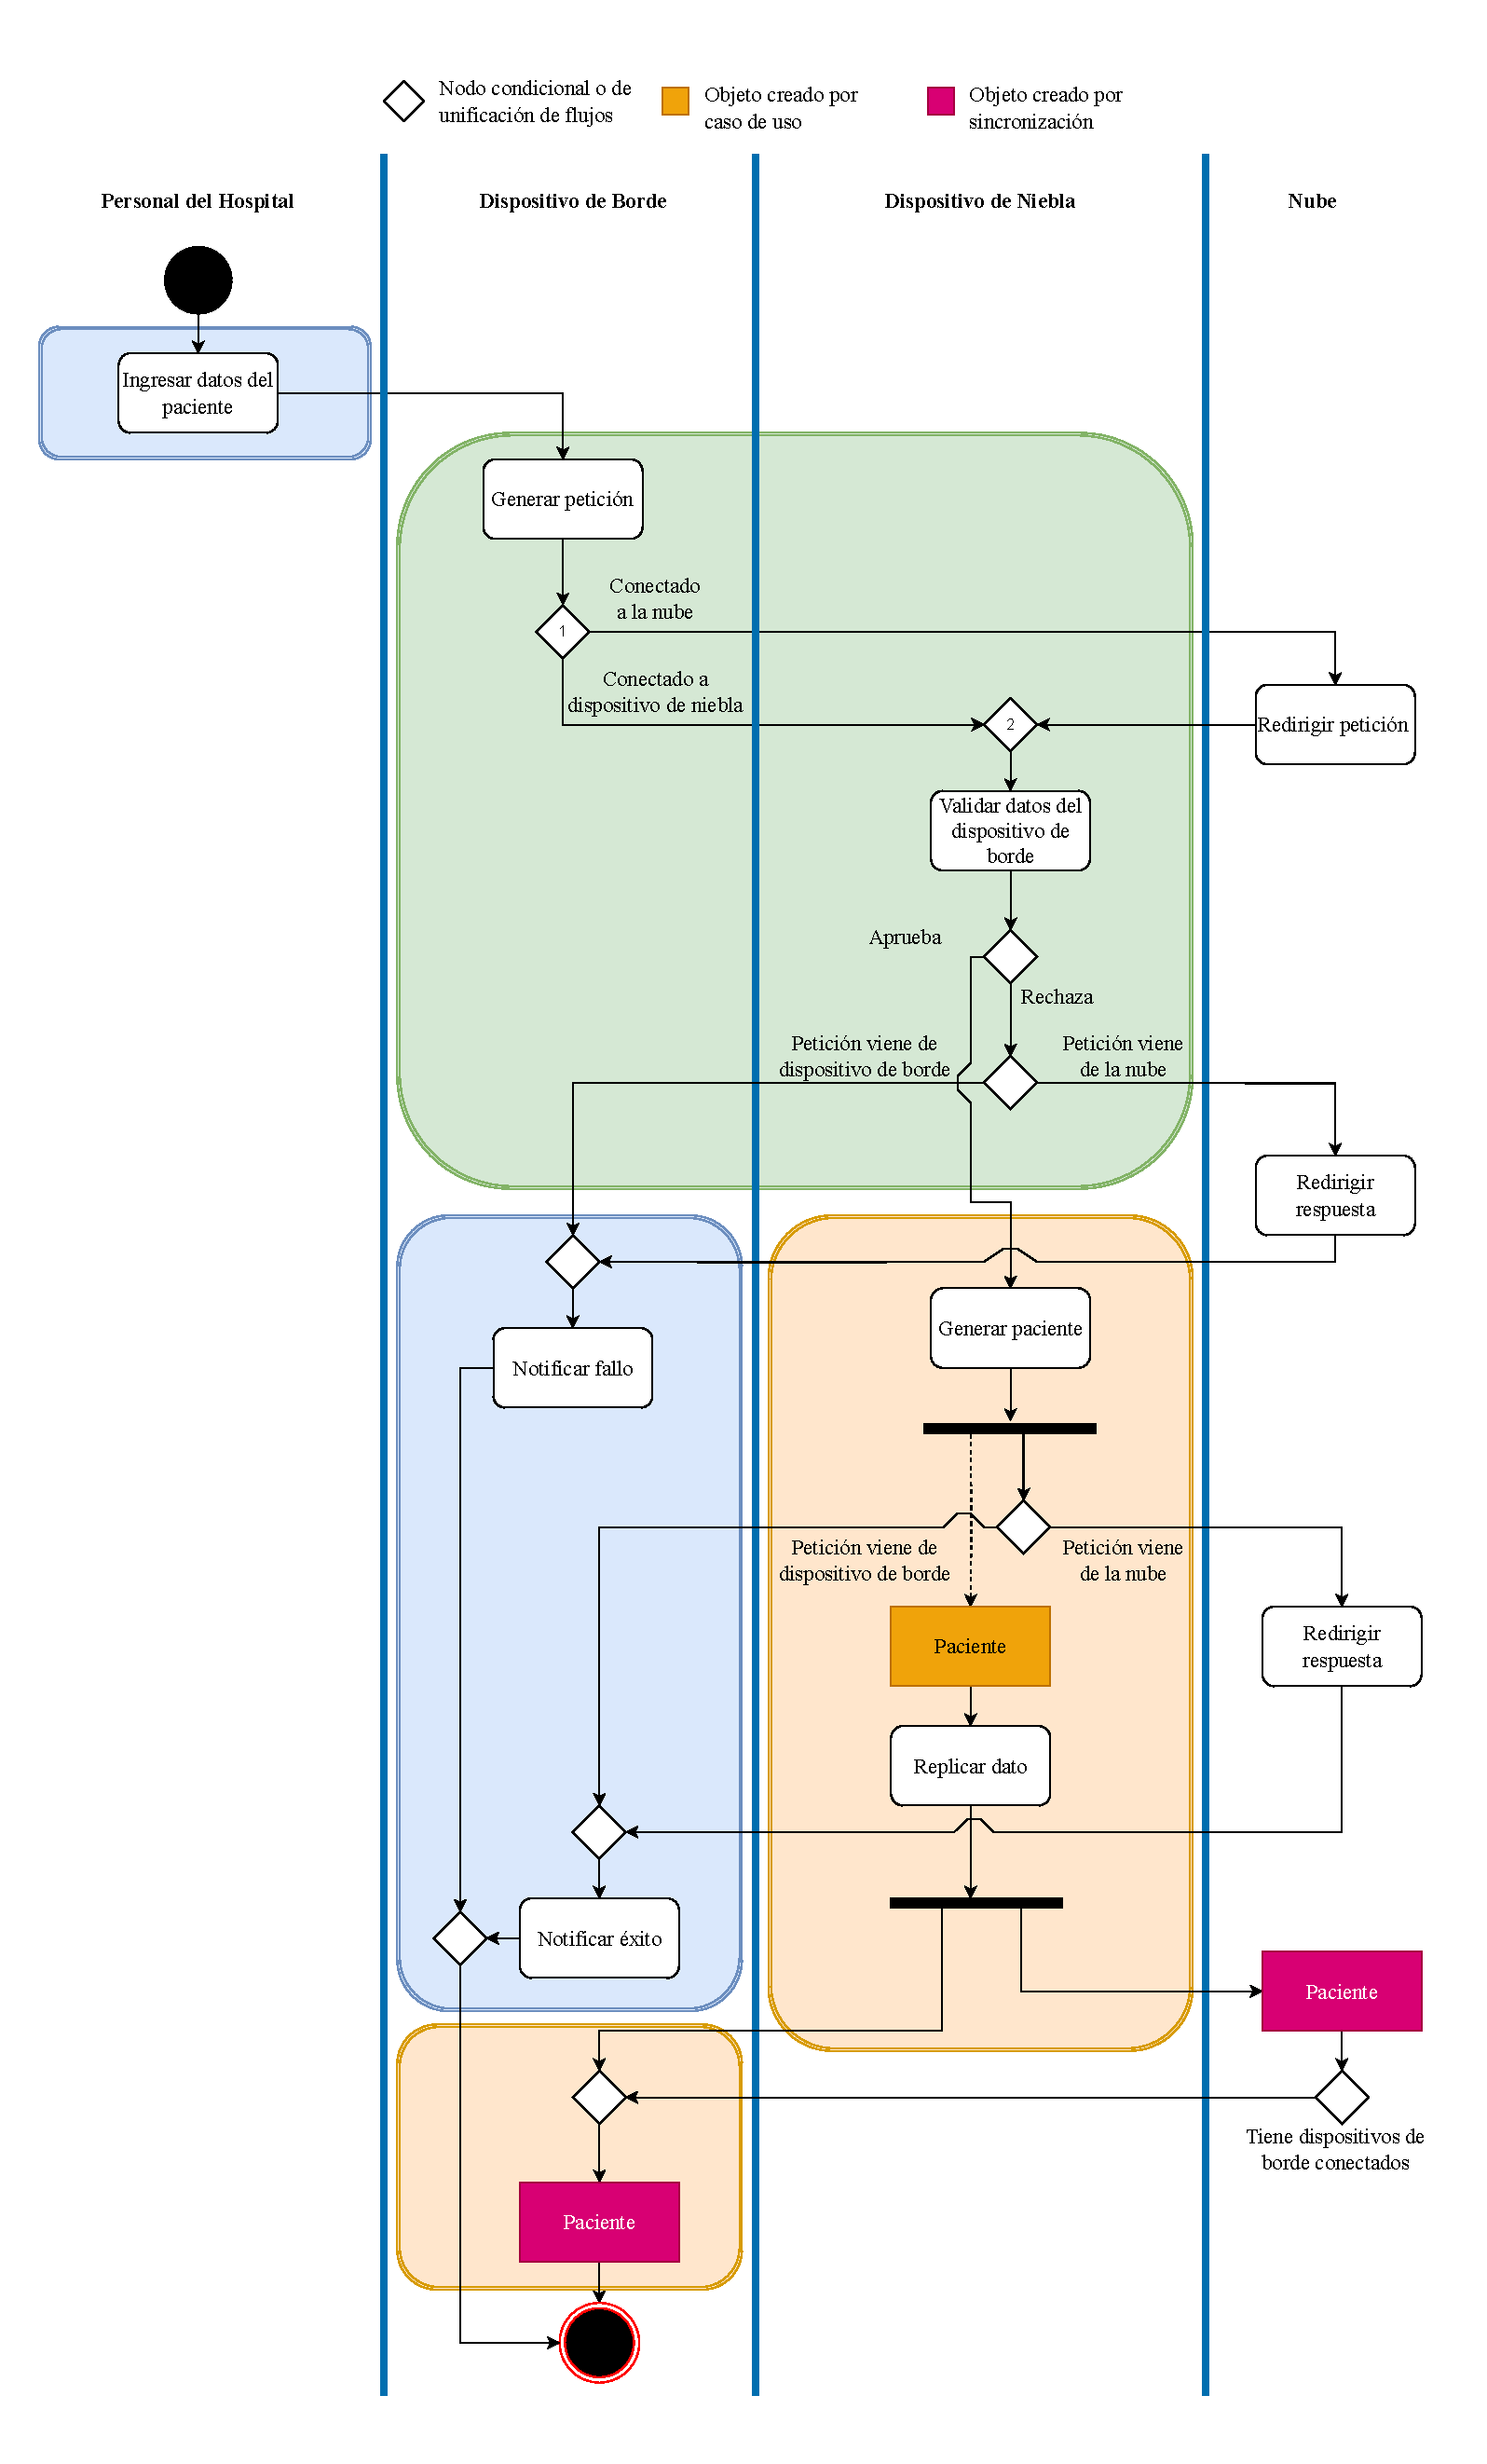
\includegraphics[width=\textwidth, height=\textheight, keepaspectratio]{Imagenes/Implementacion/DetalladoIngresarPaciente.pdf}
    \caption{Diagrama de actividades del caso de uso \textit{Admisión Paciente}}
    \label{fig:diagActAdmPaciente}
\end{figure}

A continuación se detalla a que componente del sistema, los cuales están especificados en la figura \ref{fig:comunCapasArquitectura}, se corresponde cada actividad del diagrama de la Figura \ref{fig:diagActAdmPaciente}:
\begin{itemize}
    \item \textbf{Interfaz gráfica:} Ingresar datos del paciente, Notificar fallo, Notificar éxito.
    \item \textbf{Caso de uso: }Generar petición, Validar datos del dispositivo de borde.
    \item \textbf{Entidades: }Validar datos del dispositivo de borde, Generar paciente.
    \item \textbf{Implementación Fuente de Datos: }Generar Paciente, Crear/Guardar registro ``Paciente''.
    \item \textbf{Implementación Servicio: }Replicar datos, transmisión entre dispositivos.
\end{itemize}

Las actividades ``Validar datos del dispositivo de borde'' y ``Generar paciente'' se corresponden a más de un componente dado que hacen uso de \textit{entidades}, las cuales son independientes de la infraestructura y pueden ser utilizadas en cualquier capa de la arquitectura.

Las comunicaciones entre el dispositivo de borde y de niebla siempre hacen uso de la implementación de un servicio al cual se accede a través de la interfaz Repositorio de la capa de \textit{datos}.

%\todo[inline]{aclaro o lo saco esto de abajo?}
%En la Figura \ref{fig:diagActAdmPaciente} se detallan dos posibles usos para el rombo:
%\begin{itemize}
%    \item \textbf{Nodo condicional}: Marca una condición que se da durante la ejecución, por ejemplo en el rombo etiquetado con 1 se analiza si el dispositivo de borde está conectado a la nube o a un dispositivo de niebla.
%    \item \textbf{Unificación de flujos}: Se utiliza para representar que dos condiciones confluyen en un mismo punto de ejecución. Por ejemplo, en el rombo etiquetado con 2 se indica que, después de que la nube redirige la petición o en caso de que el dispositivo de borde esté conectado al dispositivo de niebla, en ambos casos se procederá a validar los datos enviados por el dispositivo de borde.
%\end{itemize}

Adicionalmente, en el Anexo \ref{Anexo: Especificacion} se encuentran los diagramas de actividades de los casos de uso \textit{Iniciar sesión}, \textit{Conectarse a dominio} y \textit{Convertir a dispositivo de niebla}. Los casos de uso \textit{Asignar cama} y \textit{Modificar datos personales paciente} son variaciones del caso de uso \textit{Admisión paciente} por lo que se opta por no especificarlos con un diagrama de actividades. Los casos de uso \textit{Ver ficha de paciente} y \textit{Ver estado camas}, consisten en realizar accesos a la base de datos local del dispositivo de borde sin la necesidad de comunicaciones con la nube o el dispositivo de niebla, dada su simplicidad no se especificaron con un diagrama de actividades.

En la Figura \ref{fig:diagClasesAdmPaciente} se detalla el diagrama de clases del caso de uso \textit{Admisión paciente}, se puede ver que el caso de uso está mencionado como \texttt{CreatePacienteUseCase} que es el nombre que se utilizó en el código. Además, se observa nuevamente como cada clase e interfaz está coloreada en función a la capa de la arquitectura a la que pertenecen.

\begin{figure}
    \centering
    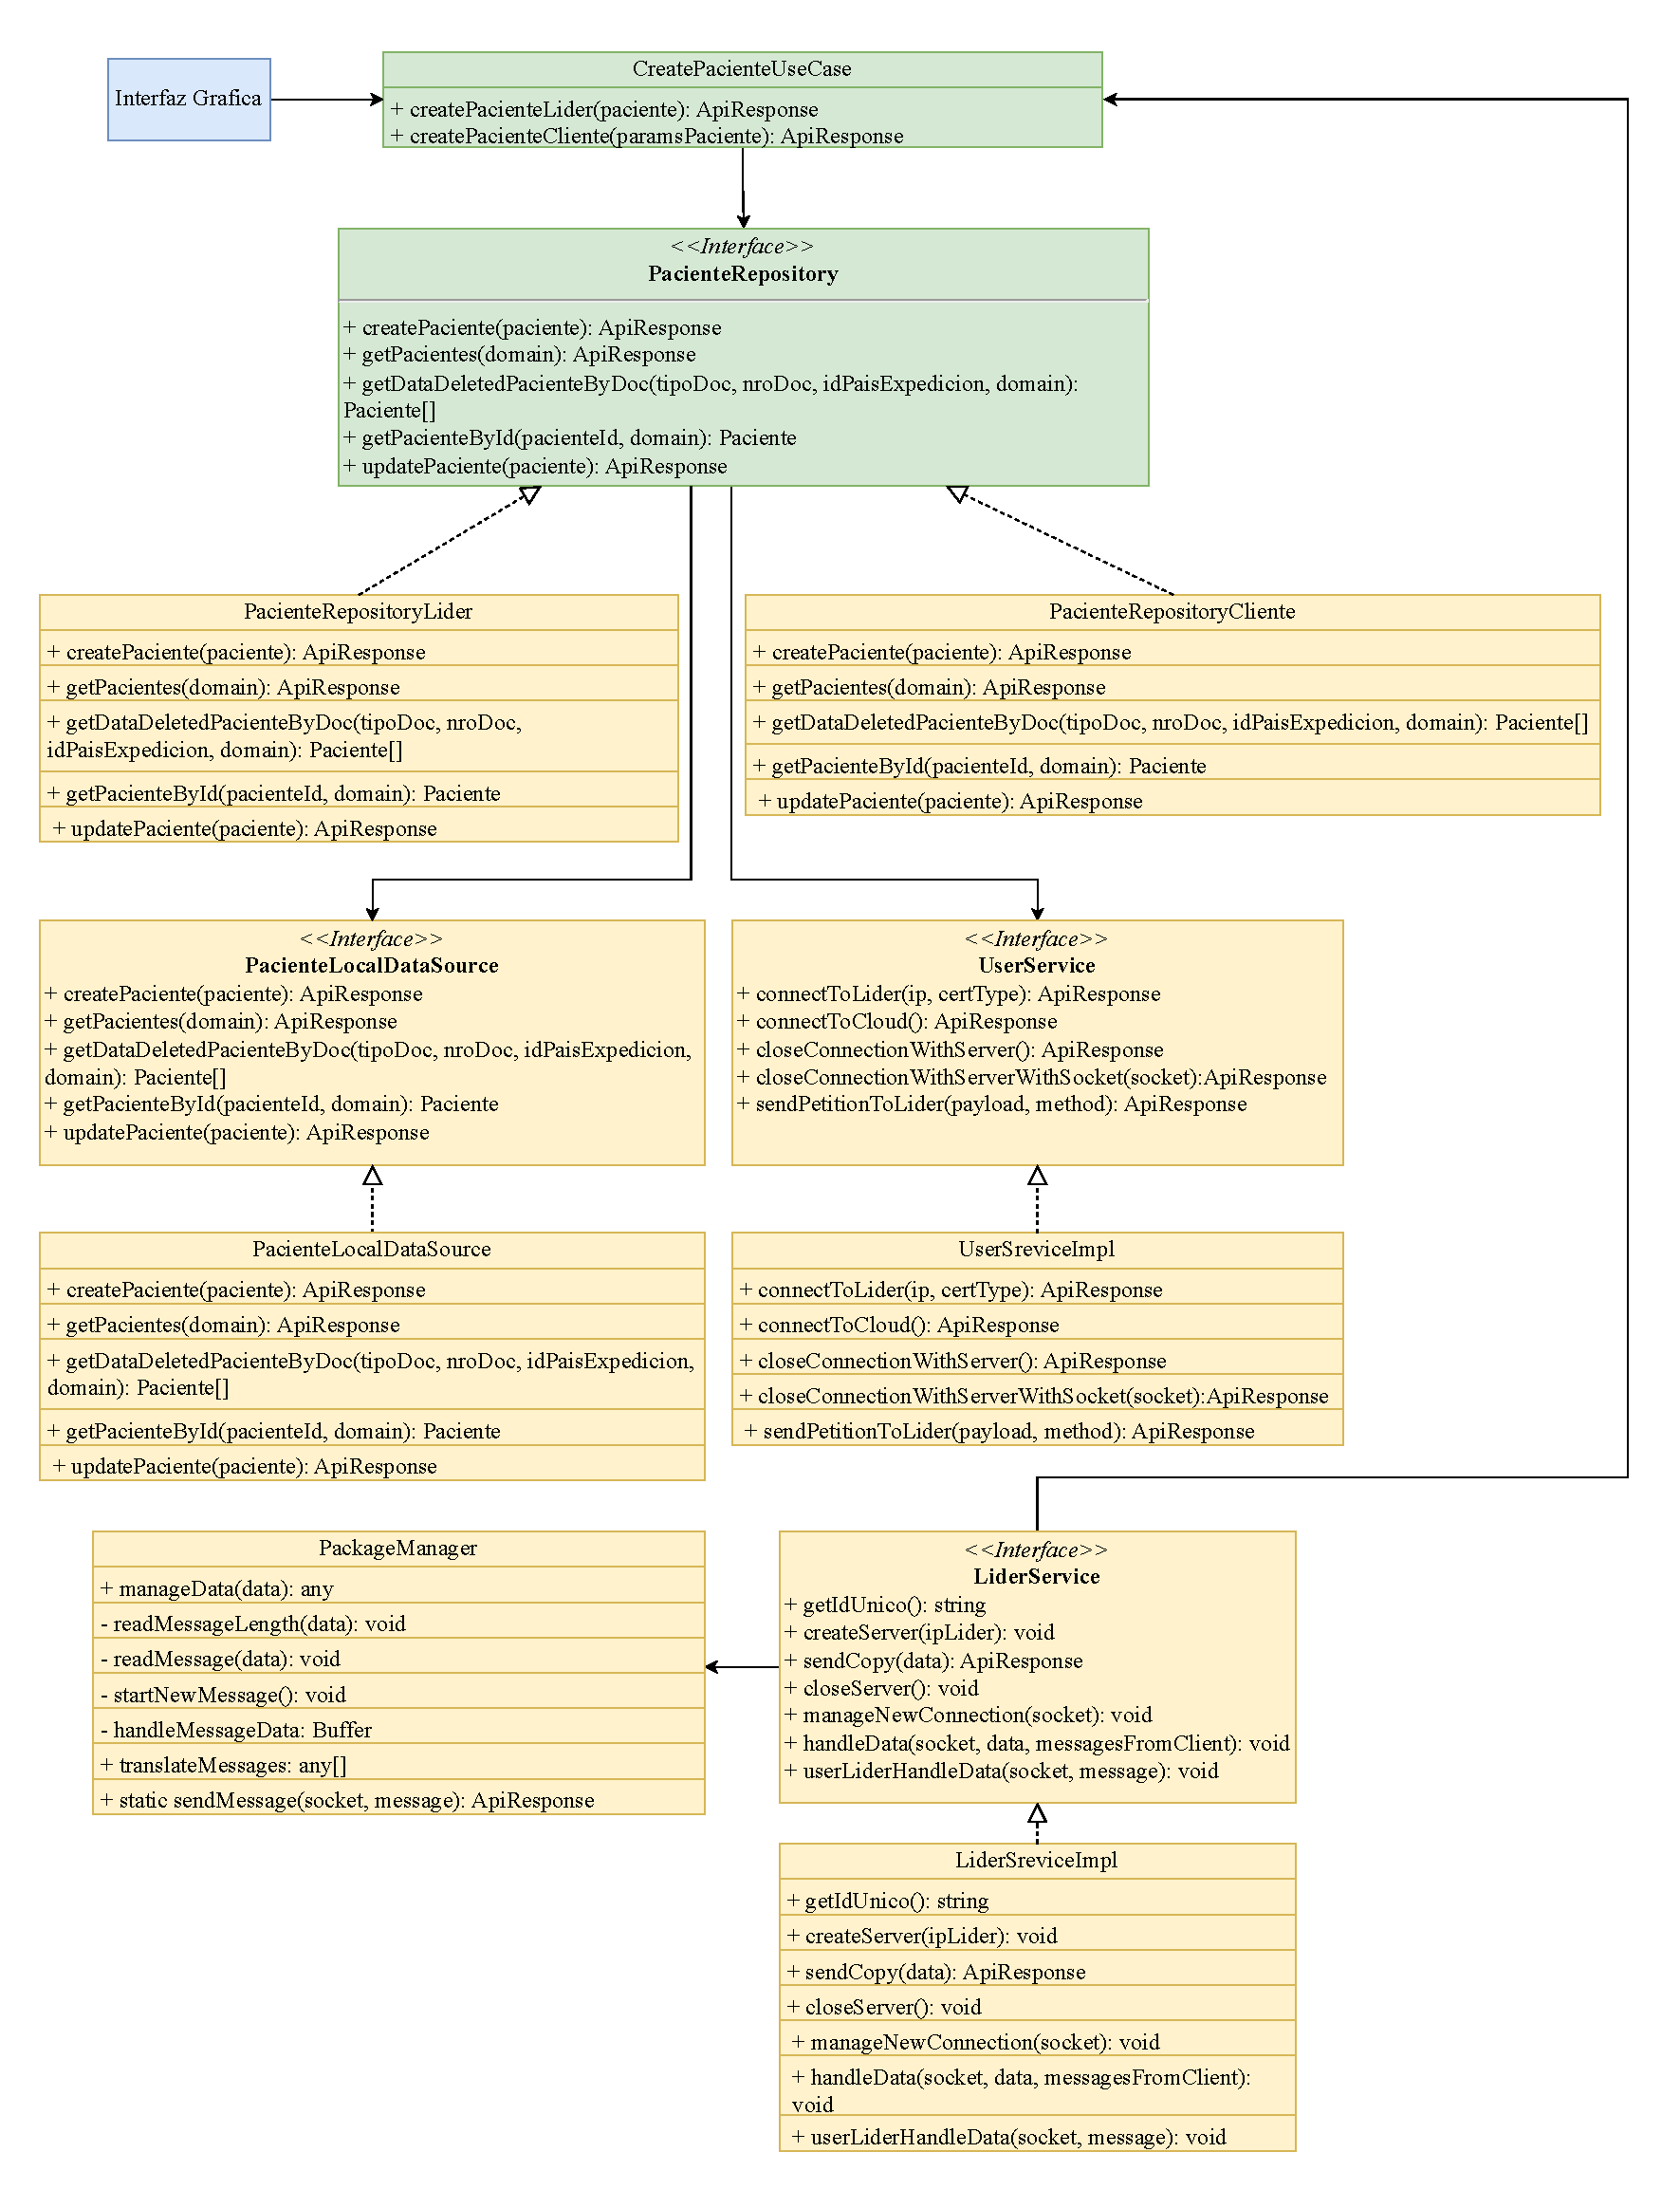
\includegraphics[width=\textwidth, height=\textheight, keepaspectratio]{Imagenes/Implementacion/DiagramaClasesAdmPaciente.pdf}
    \caption{Diagrama de clases del caso de uso \textit{Admisión Paciente}}
    \label{fig:diagClasesAdmPaciente}
\end{figure}

A continuación se procede a explicar el caso de uso \textit{Admisión paciente} con el diagrama de clases de la Figura \ref{fig:diagClasesAdmPaciente}, ademas es recomendable considerar la especificación del diagrama de actividades de la Figura \ref{fig:diagActAdmPaciente}:

\begin{enumerate}
    \item A través de la \textbf{interfaz gráfica}, el usuario utiliza el caso de uso con el método\\ \texttt{createPacienteCliente} de la clase \textbf{CreatePacienteUseCase}.
    
    \item El método \texttt{createPacienteCliente} realiza la actividad ``Generar petición'' y la envía a través de \textbf{UserServiceImpl} con el método \texttt{sendPetitionToLider}. Para el envío se hace uso del repositorio \textbf{PacienteRepositoryCliente} como intermediario entre el caso de uso y el servicio.

    \item El dispositivo de niebla recibe la petición en el método \texttt{handleData} de \textbf{LiderServiceImpl}, el cual contiene el socket del servidor a través del cual recibe los mensajes. Luego, interpreta el mensaje haciendo uso de \textbf{PackageManager} y ejecuta el caso de uso con el método\\ \texttt{createPacienteLider}, el cual se encarga de realizar la tarea ``Validar datos del dispositivo de borde''.

    \item El dispositivo de niebla, a través del repositorio \textbf{PacienteRepositoryLider}, utiliza el método \texttt{createPaciente} correspondiente a la implementación \textbf{PacienteLocalDataSource} el cual realiza las tareas de ``Generar Paciente'' y almacenarlo localmente.

    \item El dispositivo de niebla envía la respuesta al de borde haciendo uso del mismo \textit{socket} previamente establecido en la conexión inicial.

    \item El dispositivo de niebla realiza la tarea de replicación de datos hacia la nube y los dispositivos de niebla que estén conectados a él, incluido el que realizó la solicitud con el método \texttt{sendCopy} de \textbf{LiderService}.

    \item Al recibir la réplica, los dispositivos de borde ejecutan el procedimiento encargado del almacenamiento de réplicas.
    
\end{enumerate}





\section{Evaluación de funcionamiento}
En la Figura \ref{fig:screensTest} se muestran las interfaces gráficas usadas para verificar el funcionamiento durante el desarrollo. Estas están compuestas por botones que se encuentran distribuidos en tres pantallas, la de \textit{Inicio de sesión}, la de \textit{Menú principal} y la de \textit{Convertir a dispositivo de niebla}.

\begin{figure}[h]
    \centering
    \begin{minipage}{.3\textwidth}
        \centering
        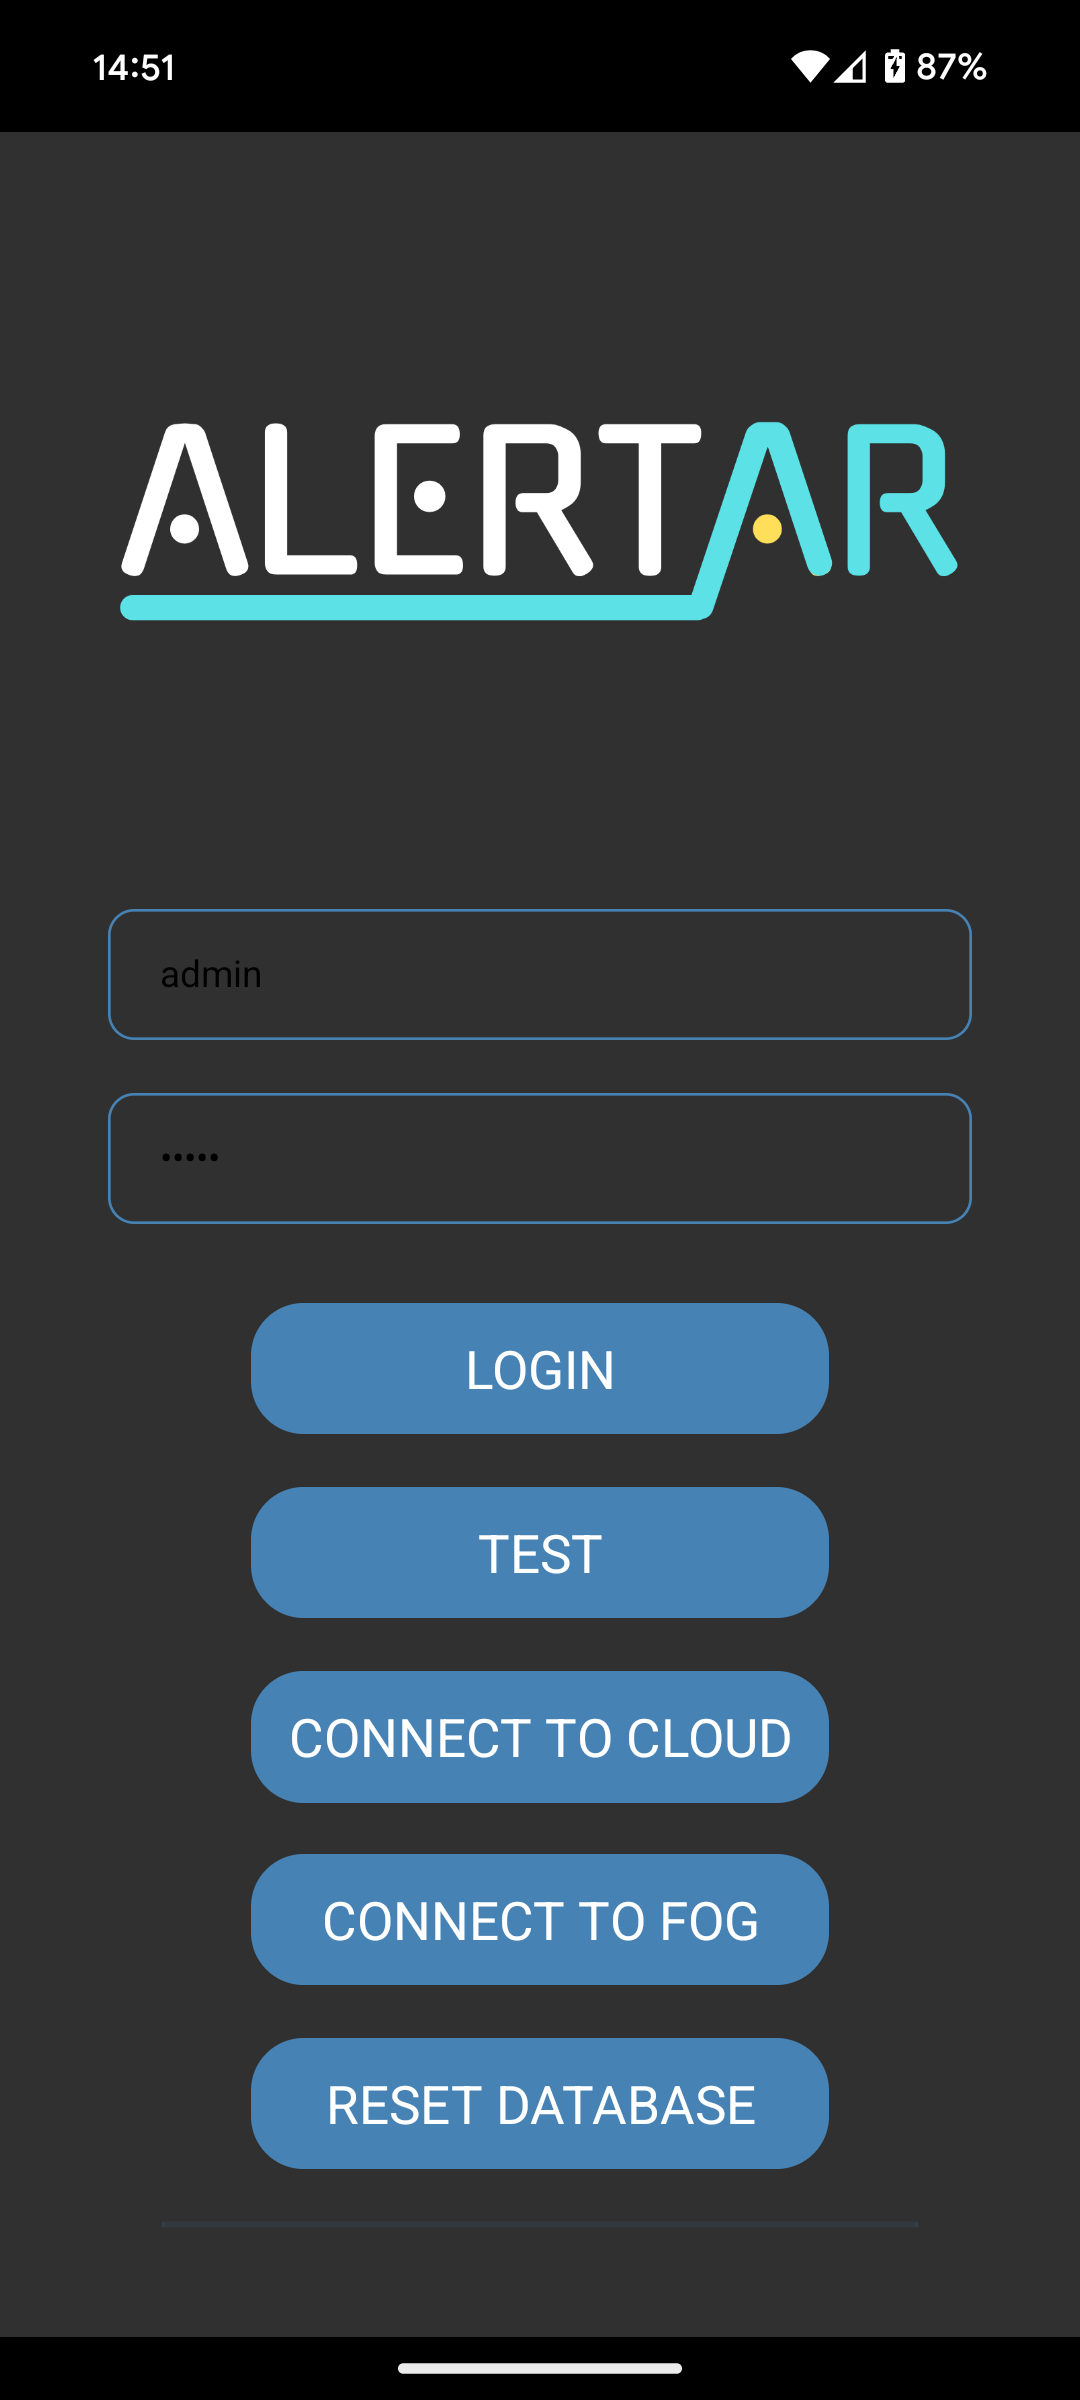
\includegraphics[width=\textwidth, keepaspectratio]{Imagenes/Implementacion/mainMenu.png}
 	
        \label{fig:screenLogin}
    \end{minipage}%
    \hfill
    \begin{minipage}{.3\textwidth}
        \centering
        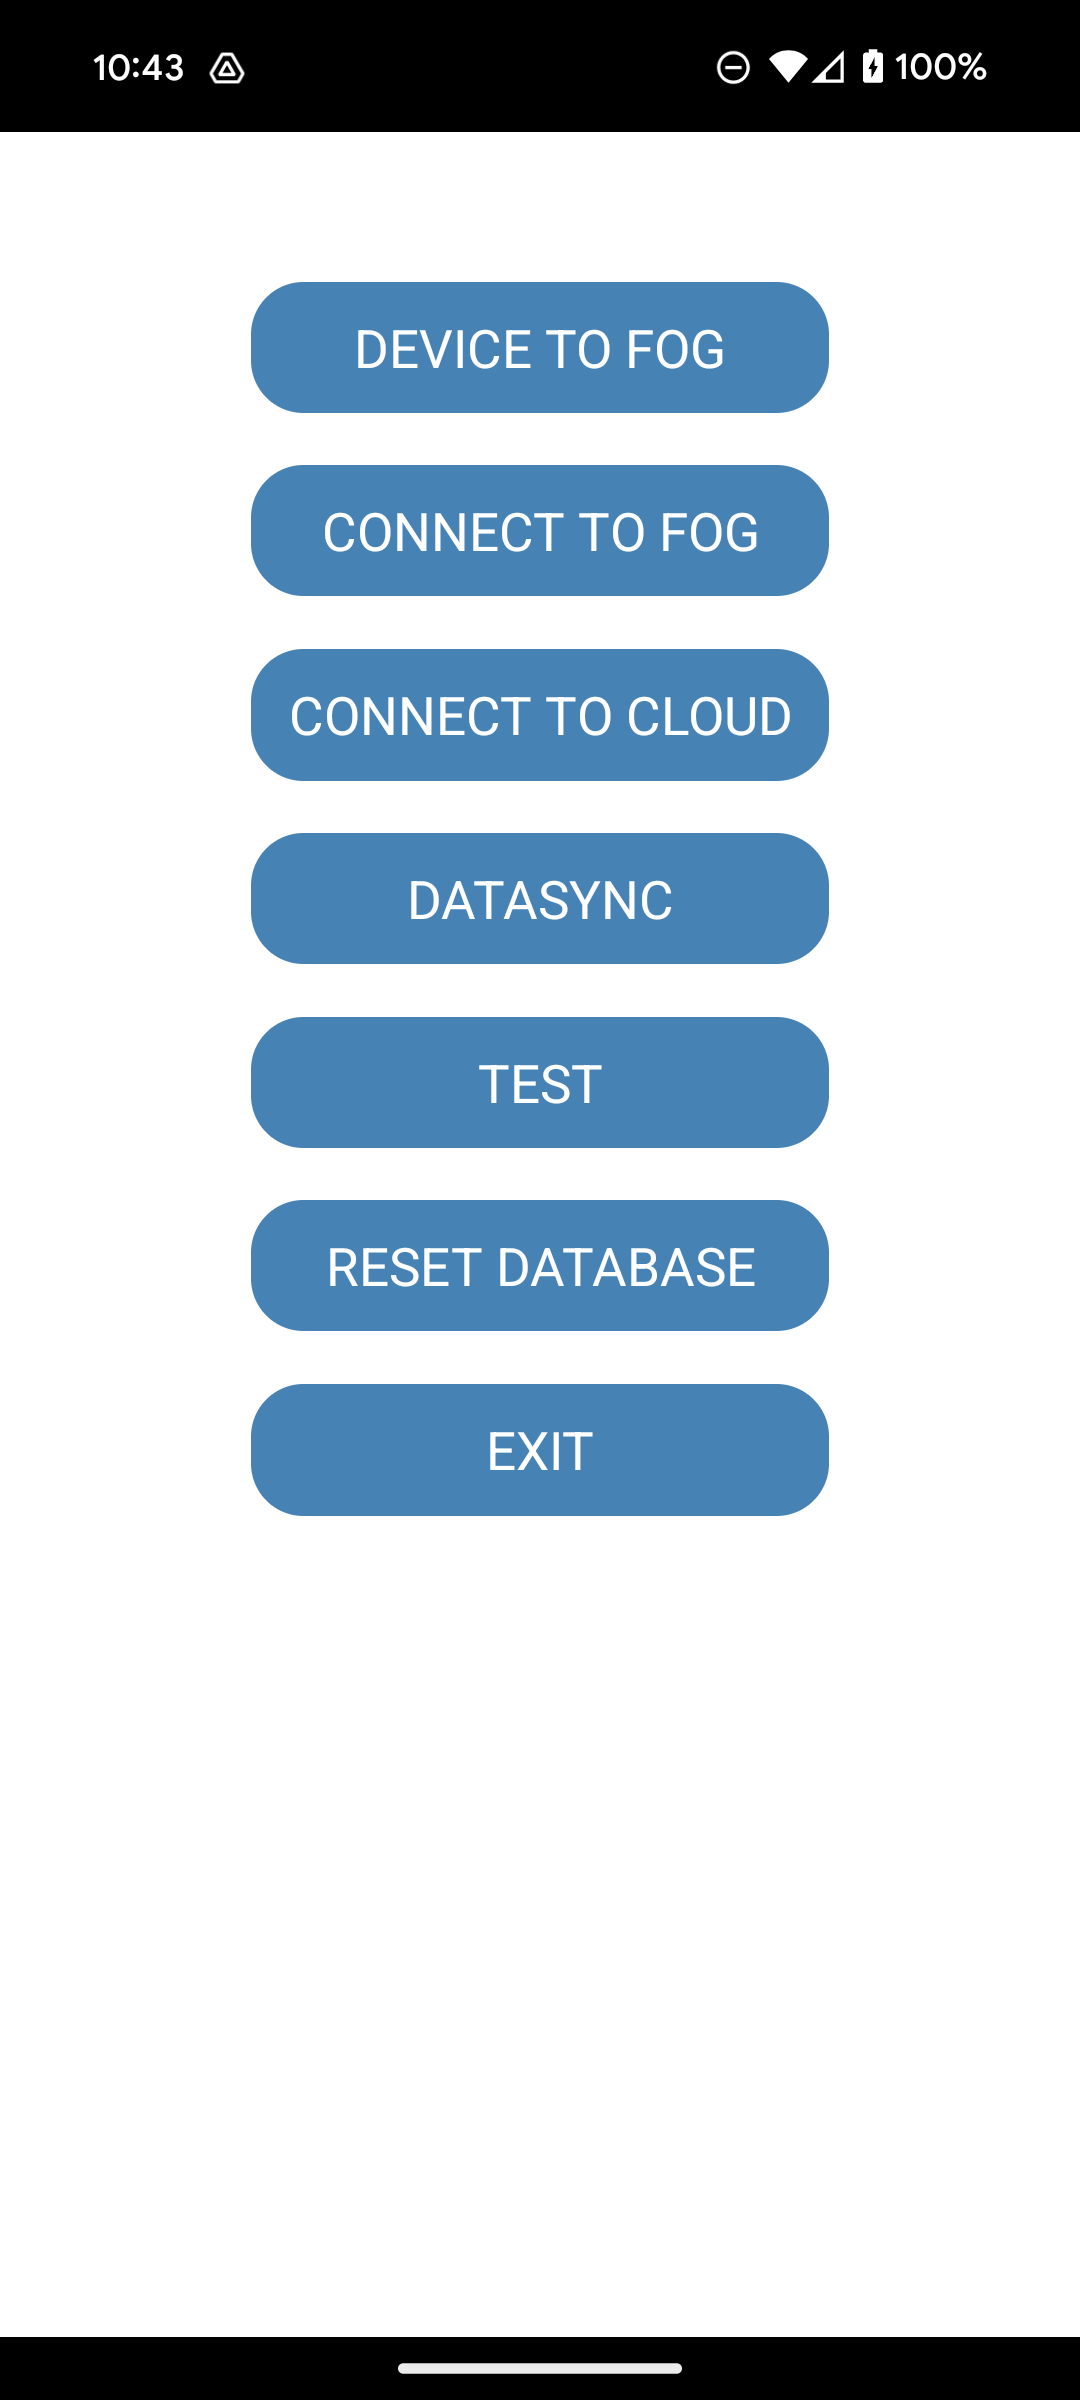
\includegraphics[width=\textwidth, keepaspectratio]{Imagenes/Implementacion/homeMenu.png}

        \label{fig:screenHome}
    \end{minipage}%
    \hfill
    \begin{minipage}{.3\textwidth}
        \centering
        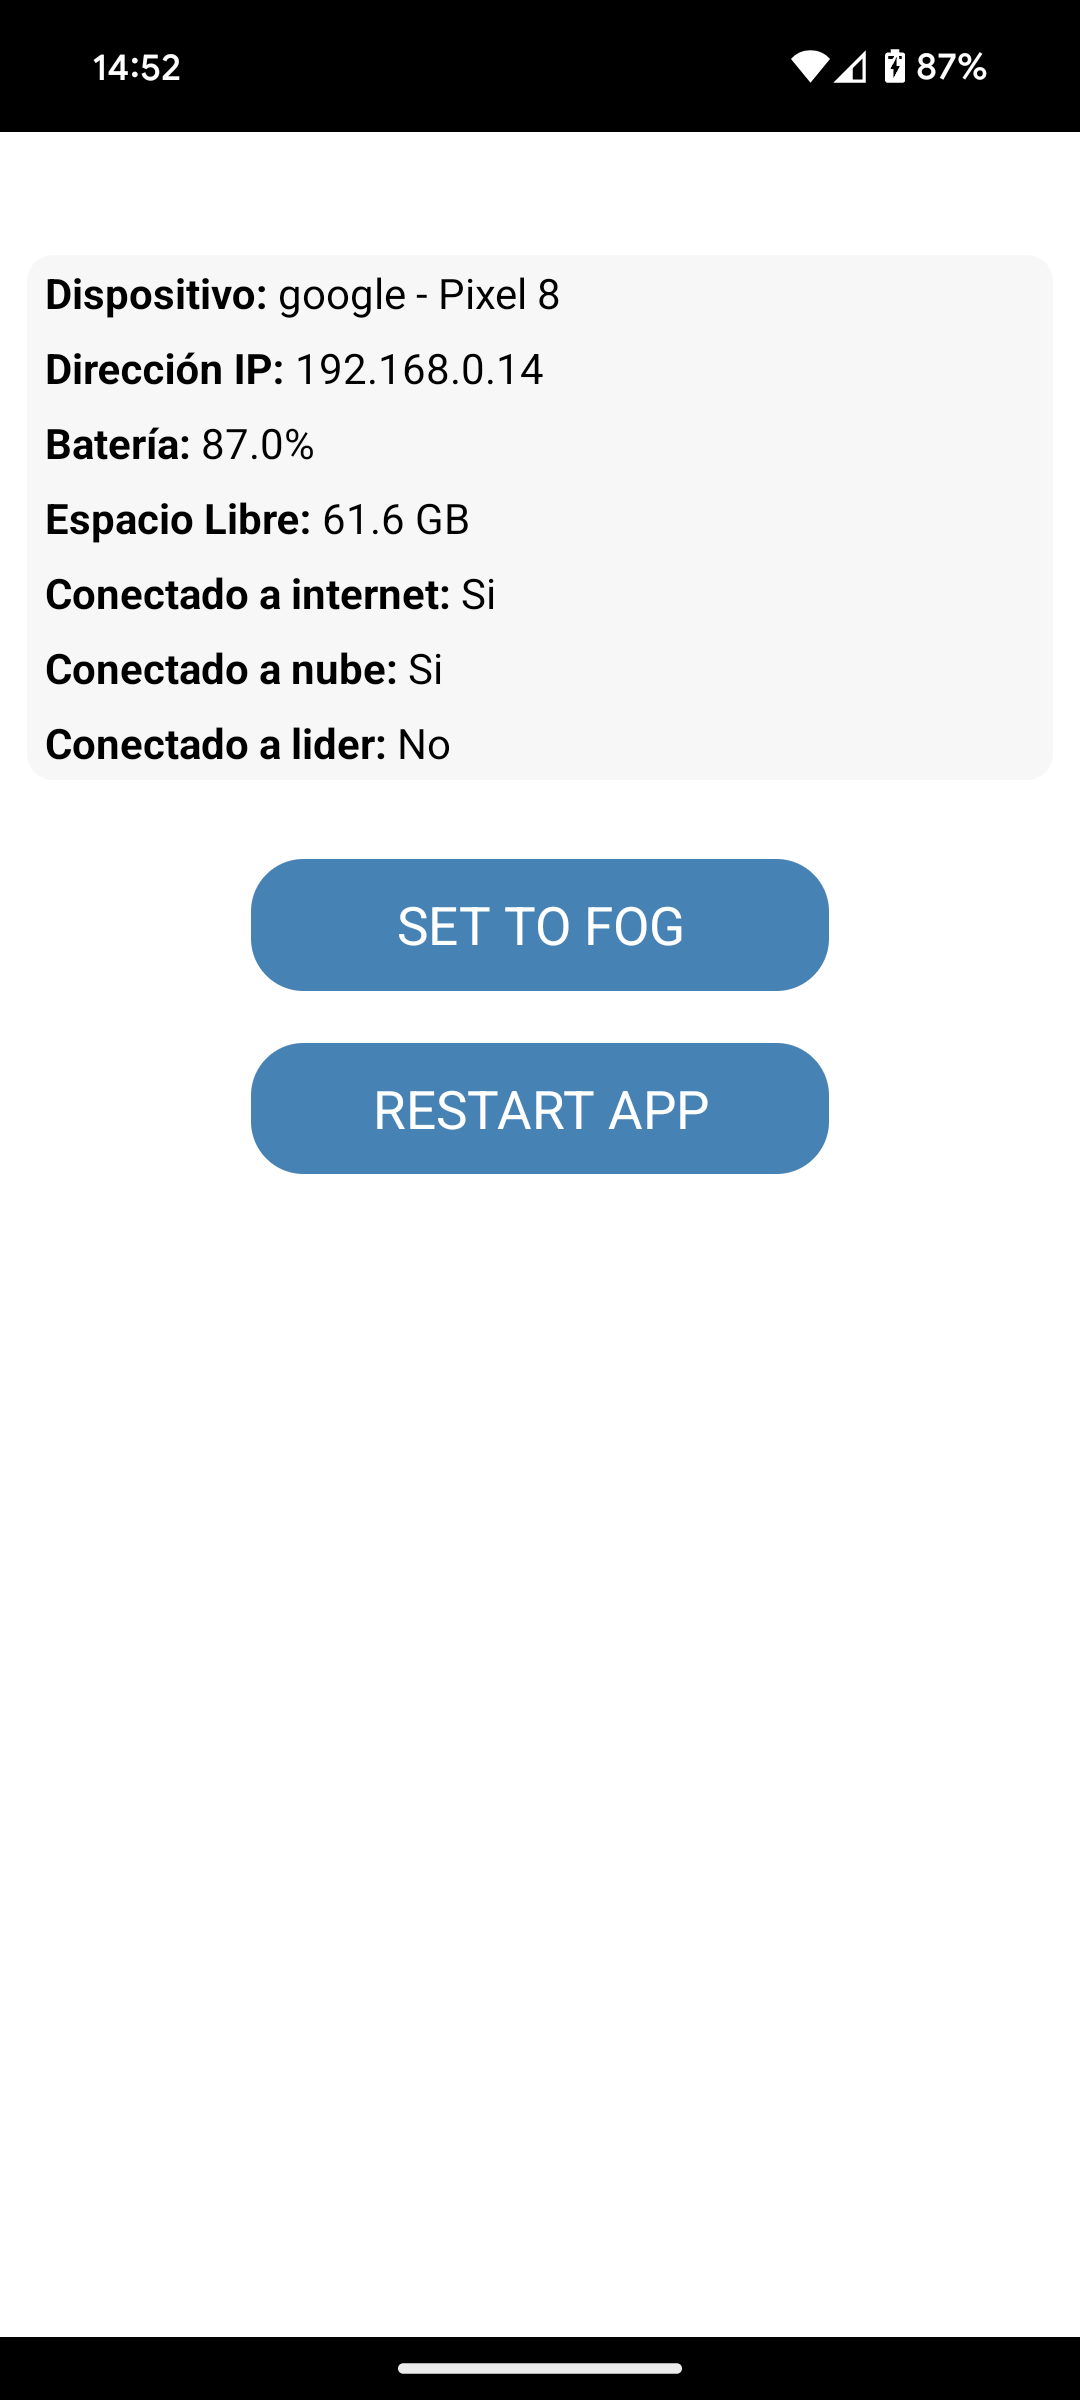
\includegraphics[width=\textwidth, keepaspectratio]{Imagenes/Implementacion/ConvertirALider.png}

        \label{fig:screenLider}
    \end{minipage}
    \caption{Pantallas \textit{Inicio de sesión}, \textit{Menú principal} y \textit{Convertir dispositivo a líder} utilizadas para la depuración en desarrollo}
    \label{fig:screensTest}
\end{figure}

Los botones al presionarse realizan acciones que derivan en llamados a casos de uso, los parámetros de estos llamados se especifican directamente en el código, evitando así la necesidad de interfaces gráficas con formularios para la carga de datos. Los botones realizan las siguientes acciones al presionarse:
\begin{itemize}
    \item \textbf{LOGIN: }ejecuta el caso de uso \textit{Iniciar sesión}.
    \item \textbf{TEST: }ejecuta un caso de uso especificado en el código para su evaluación.
    \item \textbf{CONNECT TO CLOUD: }realiza una conexión entre el dispositivo de borde con la nube.
    \item \textbf{CONNECT TO FOG: }realiza una conexión entre el dispositivo de borde con el dispositivo de niebla. Para esto, debe existir un dispositivo de niebla al cual conectarse, y el de borde ya debe tener el certificado e \textit{IP} del dispositivo de niebla para realizar la conexión.
    \item \textbf{RESET DATABASE: }restaura la base de datos a su estado original sin registros, excepto los registros correspondientes a los relojes lógicos de cada dominio que están inicializados en cero.
    \item \textbf{DEVICE TO FOG:} transición desde la pantalla \textit{Menú principal} a la pantalla  \textit{Convertir a dispositivo de niebla}.
    \item \textbf{SET TO FOG: }ejecuta el caso de uso \textit{Convertir a dispositivo de niebla}.
    \item \textbf{CLOSE CONNECTION: }desconecta al dispositivo de niebla, provocando que se corte la conexión de todos los dispositivos de borde y la nube con este.
    \item \textbf{DATASYNC: }el dispositivo de borde envía una solicitud para la sincronización de datos a la nube o al dispositivo de niebla al cual esté conectado.
    \item \textbf{EXIT: }transición desde la pantalla \textit{Menú principal} a la pantalla  \textit{Inicio de sesión}.
\end{itemize}


\subsection{Evaluación de la arquitectura}
Como se muestra en la Figura \ref{fig:arqGeneral} existen diferentes tipos de conexiones entre los componentes de la arquitectura. A causa de esto, se producen diferentes escenarios en cuanto al funcionamiento del sistema y estado de los datos. Los componentes del sistema pueden estar completamente operativos o algunos pueden fallar, en respuesta a esto el sistema debe mantenerse resiliente.

Los posibles escenarios se presentan en la Tabla \ref{tabla:evArq} y los resultados de la evaluación de cada uno fue positiva. En esta tabla, los dispositivos de borde se denominan "Borde", los dispositivos de niebla se mencionan como "Niebla", y los dispositivos que aún no tienen conexión se identifican simplemente como "Dispositivos".

En la primera columna se detalla, de manera resumida, el procedimiento que se está realizando a nivel núcleo de la aplicación. En la segunda columna se indica el tipo de conexión del dispositivo borde con el que se está operando, este puede estar conectado a la nube o a un dispositivo de niebla. En la tercera columna se contempla si existe conexión entre la nube y el dispositivo de niebla. En la cuarta columna se detalla el resultado esperado, que indica el estado de las bases de datos de los dispositivos participantes finalizado el procedimiento y, en caso de ser necesario, pasos intermedios que se deben cumplir antes de finalizar.


\begin{table}[h]

\captionof{table}{Evaluación del funcionamiento de la arquitectura}
\label{tabla:evArq} 
\begin{tabular}{|m{5cm}|m{2.5cm}|m{2cm}|m{5cm}|} \hline           
    \centering\textbf{Procedimiento} & \centering\textbf{Tipo conexión} & \centering\textbf{Hay conexión Nube $\Leftrightarrow$ Niebla} & \begin{center}
        \textbf{Resultado esperado}
    \end{center}  \\
    
    \hline Dispositivo se conecta a la nube, hace el \textit{dataSync}, se convierte en Niebla de un sector & Borde $\Leftrightarrow$ Nube & Sí & Se copia la BD de la nube en el nuevo dispositivo Niebla  \\ 
    %\hline El líder hace un \textit{insert} de un paciente & Cliente $\Leftrightarrow$ Nube & Sí & Se inserta un nuevo paciente en líder, nube y clientes & OK \\ 
    \hline El dispositivo de Borde hace un \textit{insert} de un paciente & Borde $\Leftrightarrow$ Nube & Sí & Se inserta un nuevo paciente en Niebla, Nube y Bordes\\
    \hline Borde hace un \textit{insert} de un paciente & Borde $\Leftrightarrow$ Nube & No & Mensaje de error ya que no hay acceso a la copia primaria de Niebla. \\
    \hline Dispositivo de borde se conecta a un dispositivo de Niebla, una vez es Borde hace \textit{dataSync} & Borde $\Leftrightarrow$ Niebla & Sí & Se copia la BD del Niebla en el dispositivo Borde \\
    %\hline Líder hace un \textit{insert} de un paciente & Cliente $\Leftrightarrow$ Líder & Sí & Se inserta un nuevo dato en líder, nube y clientes & OK \\
    \hline Borde hace un \textit{insert} de un paciente & Borde $\Leftrightarrow$ Niebla & Sí & Se inserta un nuevo paciente en Niebla, nube y Bordes \\
    \hline Borde hace un \textit{insert} de un paciente & Borde $\Leftrightarrow$ Niebla & No & Se inserta un nuevo paciente en Niebla y Bordes. Una vez que se restablece la conexión Nube $\Leftrightarrow$ Niebla, se sincroniza el dispositivo de niebla con la nube \\
    \hline\end{tabular} 

\end{table}

\subsection{Evaluación del mecanismo de detección de pérdida de conectividad}
    En la Figura \ref{fig:testConexion} se presentan los diferentes tipos de conexión y los posibles fallos en el sistema ALERTAR. Estos fallos pueden ocurrir en la nube, en las conexiones o en los dispositivos móviles que actúan como bordes o niebla. Los fallos en la nube o en los dispositivos móviles se consideran como una interrupción total de sus servicios, esto ocurre cuando se cierra la aplicación, cuando un dispositivo se queda sin batería o algún otro tipo de fallo no relacionado a la conectividad. Por otro lado, los fallos de conexión se deben a la pérdida de conectividad de cada dispositivo. Por ejemplo, si un dispositivo pierde señal o se queda sin datos, se considera una falla en su lado de la conexión.
    
    \begin{figure}
        \centering
        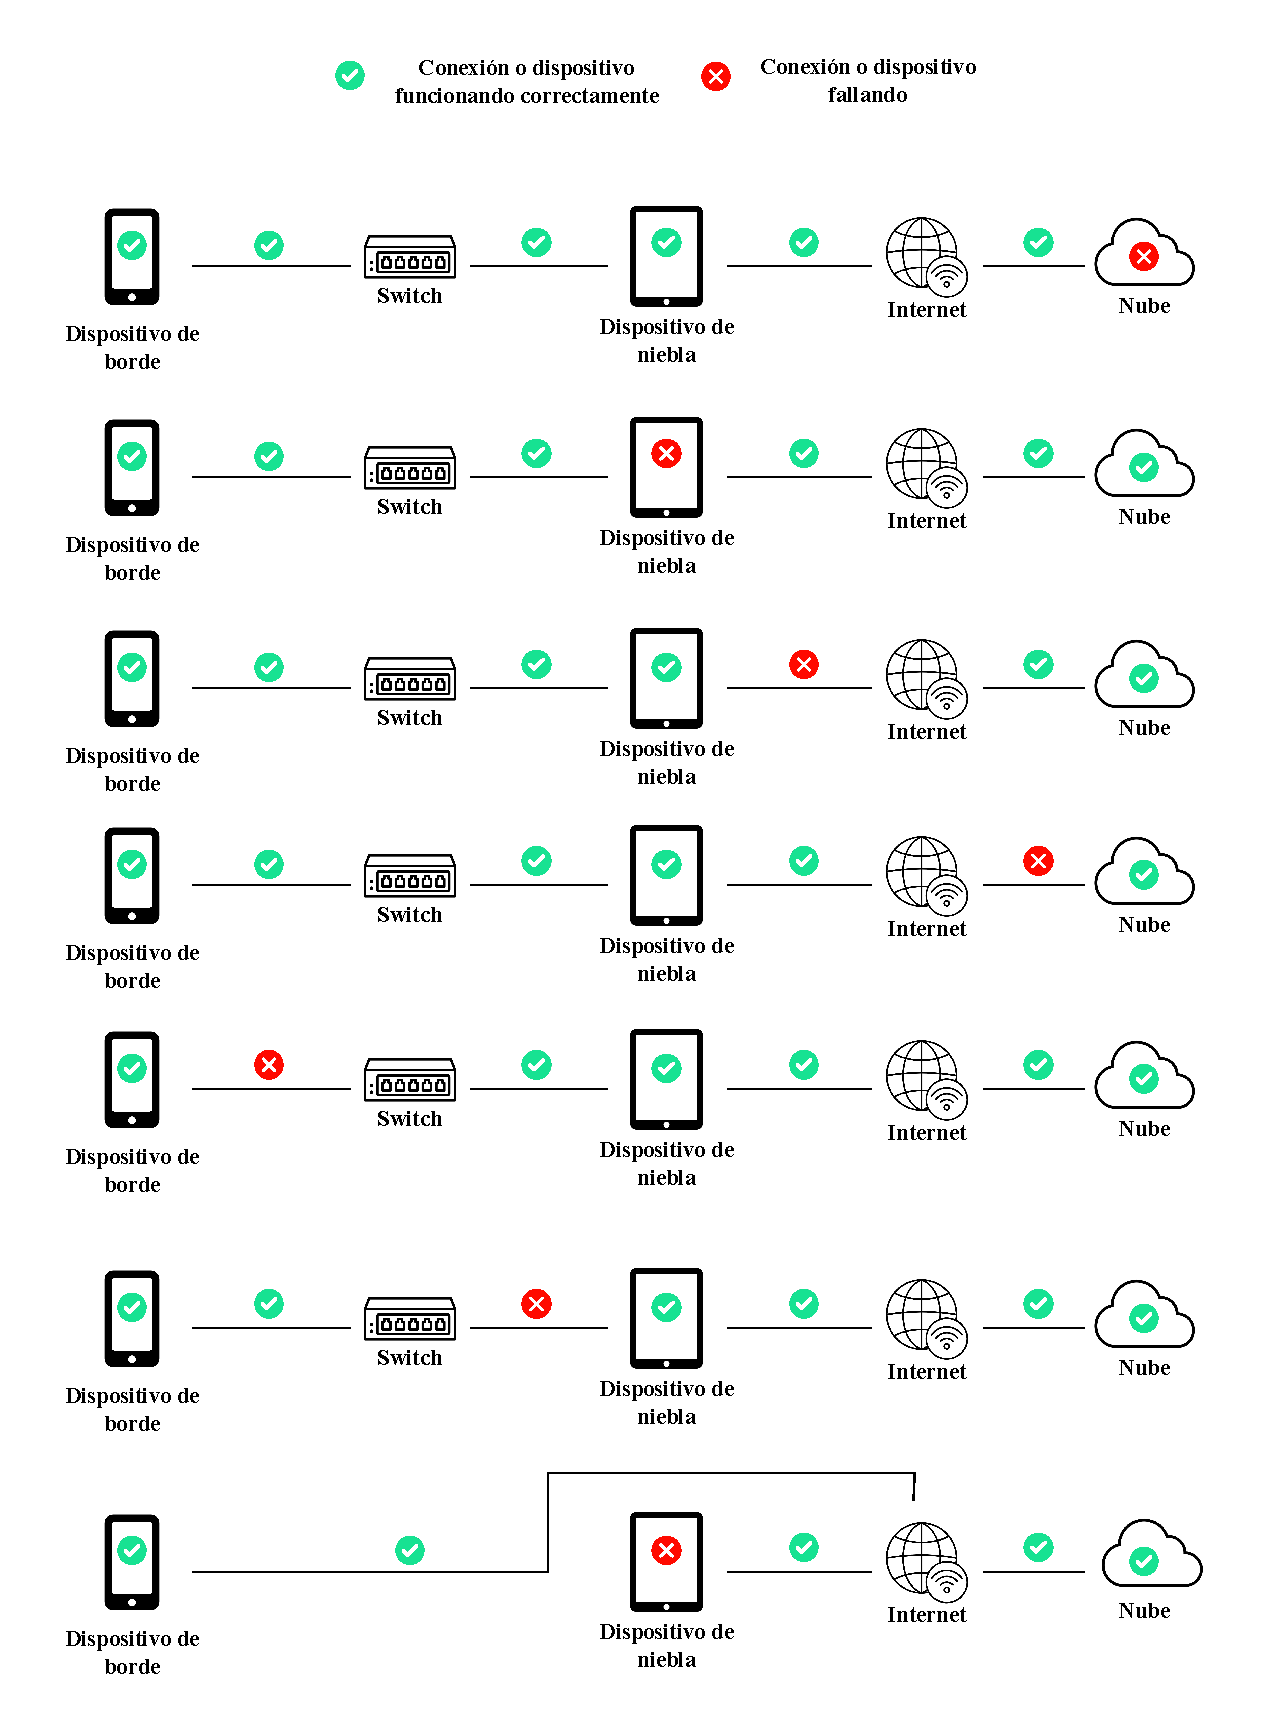
\includegraphics[width=\textwidth, height=\textheight, keepaspectratio]{Imagenes/Test/Conexiones.pdf}
        \caption{Tipos de conexión y sus posibles fallos en el sistema ALERTAR}
        \label{fig:testConexion}
    \end{figure}
    
    Se evaluaron todas las posibles combinaciones de fallos. Siempre se comenzó con el sistema totalmente operativo, luego se forzó uno por uno los diferentes tipos de fallos y se verificó que los dispositivos móviles fueran capaces de detectarlos. Posteriormente, se restableció el funcionamiento para comprobar que el sistema se recupera adecuadamente y volviera a estar operativo.
    
    A partir de esta evaluación se verificó que el mecanismo de detección de pérdida de conectividad y recuperación implementado en dispositivos móviles funciona correctamente, asegurando la recuperación del sistema ante fallos de dispositivos o conectividad.

\section{Mejoras al diseño arquitectónico}

El desarrollo de este prototipo básico permitió identificar diversas necesidades y aspectos a mejorar en el diseño arquitectónico. A través de la experiencia práctica de implementación, se detectaron ciertas limitaciones y oportunidades de mejora de diseño que pueden guiar futuras iteraciones del sistema.

\subsubsection{Separación de responsabilidades en la capa de datos}

Durante la implementación se observó que la capa de datos concentra responsabilidades heterogéneas que podrían beneficiarse de una mayor separación. Específicamente, la gestión de comunicaciones de red (como el manejo de sockets, conexiones TLS y protocolos de transporte) se encuentra mezclada con las responsabilidades relativas a una capa de datos, es decir acceso a bases de datos, repositorios y fuentes de datos. Esta mezcla dificulta el mantenimiento y la evolución independiente de estos aspectos.

Una mejora arquitectónica sería considerar la separación de las responsabilidades de comunicación de red en una capa específica, permitiendo que la capa de datos se enfoque exclusivamente en la gestión de datos y persistencia.

\subsubsection{Acoplamiento entre casos de uso y repositorios}

El diseño actual presenta múltiples repositorios específicos por separado. Esto implica la necesidad de especificar transacciones de base de datos sobre la implementación de estos repositorios. Estas transacciones son necesarias para ejecutar, de forma atómica, operaciones que involucren múltiples repositorios o fuentes de datos. De esta forma, el repositorio asume responsabilidades que trascienden su función primaria de orquestación de casos de uso, ya que se adentra en el manejo directo de detalles técnicos de persistencia. Esta mezcla de responsabilidades genera un acoplamiento fuerte entre la lógica de negocio y los mecanismos específicos de almacenamiento y acceso a datos ya que se violan los principios de responsabilidad única y separación de capas.

Dada la necesidad de manejar transacciones que involucren múltiples repositorios, se podría considerar la introducción de un gestor de repositorios. Este componente adicional se encargaría de coordinar las operaciones entre los diferentes repositorios mediante transacciones de negocio atómicas, permitiendo que cada uno mantenga su enfoque en la gestión de datos sin asumir responsabilidades técnicas relacionadas con la gestión de transacciones de bases de datos o detalles específicos de persistencia.

%todo DUDA: queda clara la diferencia entre transaccion de negocio y transacción de base de datos?
%\subsubsection{Gestión de roles de dispositivos en casos de uso}

%Durante el desarrollo se evidenció que los dispositivos de niebla y de borde presentan comportamientos distintos al ejecutar los mismos casos de uso. La implementación actual maneja estas diferencias dentro de cada caso implementando un método específico para cada tipo de dispositivo (niebla o borde), lo que genera complejidad a la hora de interpretar el código y flujo del sistema.

%Una aproximación alternativa sería considerar implementaciones específicas de casos de uso para cada tipo de dispositivo haciendo uso de una interfaz, permitiendo una lógica más clara y mantenible para cada contexto de ejecución.

\chapter{Experimentación}\label{cap:experimentacion}

El objetivo de estos experimentos es analizar el rendimiento de la aplicación móvil ALERTAR en términos de almacenamiento, transmisión de datos, tiempos de operación y conectividad entre dispositivos. Para lograrlo, se realizaron mediciones y comparaciones entre el espacio requerido y el espacio real que ocupan los datos, junto con los tiempos de transmisión de estos.

El dispositivo utilizado como borde es un \textit{Samsung Galaxy Tab A7 Lite} con un procesador \textit{Qualcomm Snapdragon 662} de \textit{2.0 GHz} con 8 núcleos, \textit{4 GiB} de memoria principal y sistema operativo \textit{Android 11}. El dispositivo utilizado como niebla es un \textit{Pixel 8} con procesador \textit{Google Tensor G3} con 9 núcleos (uno de \textit{2.9 GHz}, cuatro de \textit{2.4GHz} y cuatro de \textit{1.7 GHz}), \textit{8 GiB} de memoria principal y sistema operativo \textit{Android 15}. La nube cuenta con un procesador Intel Xeon CPU E5-2630 de \textit{2.3 GHz} y \textit{16 GB} de memoria principal y sistema operativo \textit{Linux}. Los dispositivos de borde y niebla se conectaron mediante una red inalámbrica de área local con un ancho de banda de entre \textit{85 mbps} y \textit{100 mbps}.

En la sección \ref{sec:datosUtilesVSalmacenamiento} se llevó a cabo una evaluación del espacio de almacenamiento requerido respecto del espacio real que ocupan los datos. En la sección \ref{sec:datosUtilesVsDatosEnTransito} se comparan los datos útiles contra los datos en tránsito para detectar sobrecargas de información. En la sección \ref{sec:tiemposDeLasOps} se desarrolla una evaluación del rendimiento de la aplicación considerando los tiempos de procesamiento individuales en los dispositivos de borde y los tiempos de procesamiento externos necesarios para recibir una respuesta desde la nube u otro dispositivo de niebla. Finalmente, en la sección \ref{sec:conectividadDispositivos} se realizó una prueba de estrés en los dispositivos de niebla para evaluar su capacidad de soportar múltiples conexiones simultáneas a través de una red de área local desde los dispositivos de borde.



\section{Datos útiles contra espacio de almacenamiento}
\label{sec:datosUtilesVSalmacenamiento}
Este experimento busca comprender la diferencia entre el tamaño requerido y real de los datos para identificar e intentar reducir la sobrecarga innecesaria a fin de, a futuro, poder optimizar el almacenamiento y mejorar el rendimiento de la aplicación. Para realizarlo se seleccionó la tabla de datos Paciente, que contiene la información personal de cada paciente y es una de las tablas con más parámetros en el sistema, lo que la convierte en un caso altamente significativo. A continuación se enumeran las consideraciones y pasos realizados para realizar la medición:
\begin{enumerate}
    \item Se calculó el tamaño requerido para cada tipo de dato. Las mediciones se detallan en la Tabla \ref{tabla:TamReqSegTipoDat} donde en la primera columna se muestra el nombre del atributo, en la segunda columna se indica el tipo de dato del atributo, y en la tercera columna se presenta el valor asignado a cada atributo. Cabe destacar que, en la tercera columna, algunas casillas están en blanco porque corresponden a tipos de datos enteros, cuyo tamaño será el mismo independientemente del valor utilizado. Se consideró que un entero ocupa 4 bytes y que cada carácter ocupa 1 byte en la base de datos. En la última columna se especifica el tamaño requerido para cada atributo en función del tipo de dato y el valor asignado. 
    
    \item A fin de analizar el impacto que tiene la inserción de diferentes tipos de registros, se insertaron registros de tipo \textit{Cama}. De esta manera, se insertaron 4000 registros de tipo \textit{Paciente}, donde cada registro requiere 136 bytes de datos útiles y 2000 registros de tipo \textit{Cama}, donde cada registro requiere 44 bytes de datos útiles. Así, al finalizar el experimento se contó con 6000 registros. 
    
    \item Se determinó el tamaño total requerido por registro. Esto se realizó comenzando con un grupo de cien registros y luego incrementando de cien en cien hasta alcanzar un total de 6000 registros. Las mediciones se hicieron cada cien registros insertados. Primero se insertaron los registros de tipo \textit{Paciente} y luego los de tipo \textit{Cama}. La base de datos inicialmente se encontraba vacía.
    
    \item Se calculó la ``sobrecarga'' que representa la diferencia porcentual entre el tamaño requerido de los registros y el tamaño final que ocupan en la base de datos. Los resultados de estas mediciones se encuentran en las Tablas \ref{tabla:TamReqYRealConOverPacientes}\ref{tabla:TamReqYRealConOverCamas}.
\end{enumerate}

%Primero, se calculó el tamaño requerido para cada tipo de dato, como se muestra en la Tabla \ref{tabla:TamReqSegTipoDat}. Para esto, se consideró que un entero ocupa 4 bytes y cada carácter ocupa 1 byte en la base de datos.

%Después de calcular el tamaño requerido por tipo de dato, se determinó el tamaño total requerido por registro. Esto se realizó comenzando con un grupo de cien registros y luego incrementando de cien en cien hasta alcanzar un total de 6000 registros.

%En tercer lugar se insertó dicha cantidad de registros en la base de datos y se midió cada cien inserciones el tamaño de la base de datos, la cual, inicialmente, se encuentra vacía. 

%Por último, se calculó la ``sobrecarga'' la cual representa la diferencia porcentual entre el tamaño requerido de los registros y el tamaño final que ocupan en la base de datos Tablas \ref{tabla:TamReqYRealConOverPacientes}\ref{tabla:TamReqYRealConOverCamas}.



En la Figura \ref{fig:DatosUtilesVsEspacio2} se muestra la sobrecarga de espacio utilizado para el almacenamiento secundario sobre las diferentes cantidades de registros. Las barras azules se corresponden con la tabla Paciente y las rojas con la tabla Cama. Se puede observar una mayor eficiencia (menor sobrecarga) a medida que el número de registros aumenta. Esto significa que, conforme se agreguen más registros, el espacio de almacenamiento será mejor aprovechado. Sin embargo, al comenzar a insertar datos a una tabla diferente, se produce un decremento significativo de la eficiencia (a partir de los 4100 registros), pasando de 70\% a 415\% de sobrecarga. Luego, la sobrecarga disminuye y, por lo tanto, la eficiencia aumenta.

Finalmente se concluye que el aprovechamiento del almacenamiento mejora con el crecimiento de los registros dentro de una misma tabla, lo que indica un uso más efectivo del espacio conforme se van ingresando datos. Sin embargo, la introducción de datos de diferentes tablas o tipos de datos provoca un aumento en la sobrecarga.
\begin{table}[]

\centering
\captionof{table}{Tamaño requerido según tipo de dato}
\label{tabla:TamReqSegTipoDat}
\begin{tabular}{|l|l|c|c|}
\hline
\textbf{Atributo} & \textbf{Tipo de dato} & \textbf{Valor utilizado} & \textbf{Tamaño requerido (bytes)} \\ \hline
sync\_id & integer & & 4 \\ \hline
domain & string & ``/hosp00/sector00'' & 16 \\ \hline
pacienteId & integer & & 4 \\ \hline
numeroHC & string & ``P0000000001'' & 11 \\ \hline
fechaIngreso & integer & & 4 \\ \hline
numeroDocumento & string & \textit{(8 dígitos ASCII)} & 8 \\ \hline
tipoDocumento & string & ``DNI'' & 3 \\ \hline
idPaisExpedicion & string & ``.ar'' & 3 \\ \hline
nombres & string & ``Francisco'' & 9 \\ \hline
apellidos & string & ``Repetto'' & 7 \\ \hline
sexo & string & ``M'' & 1 \\ \hline
calle & string & ``Av.Argentina'' & 12 \\ \hline
numero & string & ``100'' & 3 \\ \hline
piso & string & ``-'' & 1 \\ \hline
idProvincia & integer & & 4 \\ \hline
idLocalidad & integer & & 4 \\ \hline
CP & string & ``8300'' & 4 \\ \hline
telefono & string & ``2995000000'' & 10 \\ \hline
telefonoFamiliar1 & string & ``2995111111'' & 10 \\ \hline
telefonoFamiliar2 & string & ``2995222222'' & 10 \\ \hline
fechaNacimiento & integer & & 4 \\ \hline
deleted & integer & & 4 \\ \hline
\multicolumn{3}{|c|}{\textbf{TOTAL}} & \textbf{136} \\ \hline
\end{tabular}

\end{table}



%\begin{figure}
%    \centering
%    \includegraphics[width=\textwidth]{Imagenes/Experimentos/Diferencia entre datos útiles contra el espacio utilizado 1.pdf}
%    \caption{Diferencia entre datos útiles contra el espacio utilizado}
%    \label{fig:DatosUtilesVsEspacio1}
%\end{figure}

\begin{figure}
    \centering
    \includegraphics[width=\textwidth]{Imagenes/Experimentos/Diferencia entre datos útiles contra el espacio utilizado 2.pdf}
    \caption{Diferencia entre datos útiles contra el espacio utilizado}
    \label{fig:DatosUtilesVsEspacio2}
\end{figure}



\section{Datos útiles contra datos en tránsito}
\label{sec:datosUtilesVsDatosEnTransito}
El fin de este experimento es determinar la sobrecarga de información que se tiene a causa de la estructura y el formato requeridos por el protocolo de comunicación \textit{JSON}. Esto incluye elementos adicionales como etiquetas, delimitadores y otros metadatos necesarios para interpretar correctamente los datos enviados. 

Para este se utilizó un registro de tipo \textit{Paciente}, el cual se detalla en la Tabla \ref{tabla:TamReqSegTipoDat}. En las mediciones realizadas se observó que en tránsito hay 577 bytes lo cual significa una sobrecarga considerable de 441 bytes para transmitir un único registro con un tamaño de 136 bytes, produciendo una sobrecarga de 324\% al utilizar el formato \textit{JSON}.

Se puede afirmar que la eficiencia de transmisión es baja, ya que el tamaño real en tránsito es casi cuatro veces el tamaño necesario. Sin embargo, toda esta sobrecarga es a causa del formato estándar \textit{JSON}, el cual facilita la interoperabilidad entre sistemas diversos, brindando beneficios en cuanto uso, lectura, compatibilidad y flexibilidad de los datos. Aunque existe una sobrecarga a causa del formato, los beneficios mencionados justifican su uso.


%\begin{figure}
 %   \centering
 %   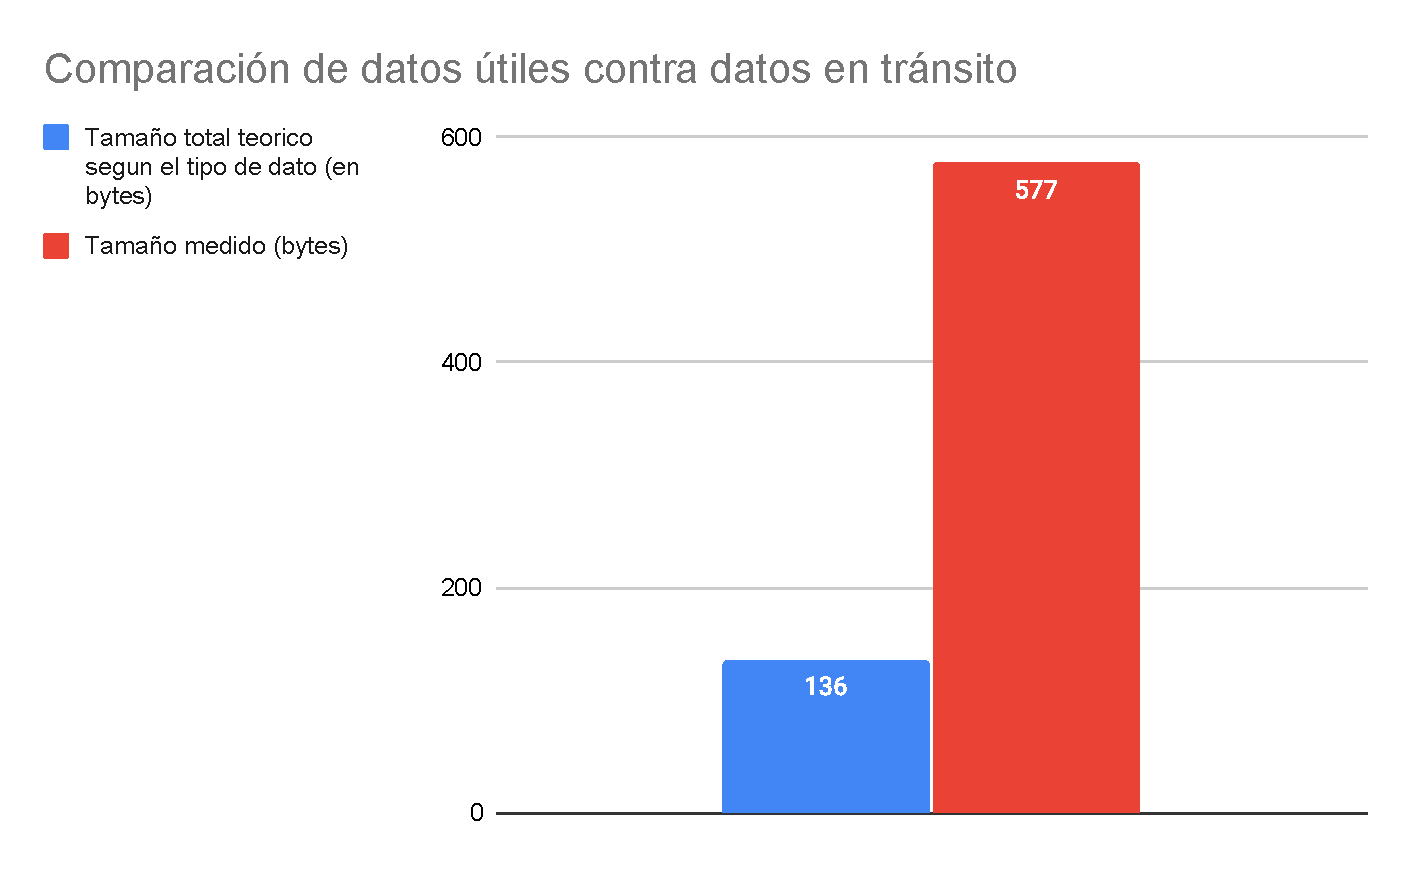
\includegraphics[width=\textwidth]{Imagenes/Experimentos/DatosUtilesVsDatosTransito.pdf}
 %   \caption{Tamaño total requerido y tamaño en tránsito}
 %   \label{fig:tamTotalvsTamTransito}
%\end{figure}
\section{Tiempos de las operaciones con diferentes tipos de conexión}
\label{sec:tiemposDeLasOps}
Este experimento se centra en evaluar y medir los tiempos de transmisión, procesamiento y el tiempo total en cada dispositivo, abarcando diversos casos de uso para las diferentes conexiones del sistema ALERTAR. El objetivo es determinar la eficiencia del sistema en completar operaciones críticas, identificar cuellos de botella donde el procesamiento puede ser excesivo, y evaluar el impacto de la latencia en las diferentes conexiones. El experimento consiste en ejecutar y medir casos de uso para los siguientes dos tipos de conexión:
\begin{itemize}
    \item \textbf{Dispositivo de borde $\leftrightarrow$ Nube: }El dispositivo de borde se encuentra conectado de manera directa a la nube. Además, existe un dispositivo de niebla a cargo del dominio al que está suscrito el de borde. Este dispositivo de niebla no participa de estas mediciones pero es necesario por requerimientos especificados en el protocolo de funcionamiento del sistema ALERTAR.
    \item \textbf{Dispositivo de borde $\leftrightarrow$ Dispositivo de niebla: }La conexión es por red de área local entre los dispositivos de borde y niebla.
\end{itemize}

Los casos de uso utilizados son los siguientes:
\begin{itemize}
    \item \textbf{Login: }Este caso de uso fue elegido debido a su complejidad en cuanto a requerimientos ya que implica hacer validaciones. En este, el dispositivo de borde envía un registro con sus datos para identificarse con el de niebla, el dispositivo de niebla se encarga de validar al usuario y como respuesta devuelve la información de los dominios a los que puede suscribirse el usuario.
    
    \item \textbf{DataSync: }Este caso de uso se eligió ya que es el encargado de sincronizar toda la información no actualizada en el dispositivo que acaba de iniciar sesión. A partir de este caso de uso se puede observar cómo se comporta el sistema a la hora de transmitir un volumen de información relativamente grande en comparación a operaciones más usuales como puede ser la inserción de un dato. Además de que permite observar cómo es el rendimiento de los dispositivos para procesar y almacenar dicha información en la base de datos.

    Durante la ejecución se hace una petición de sincronización desde el dispositivo de borde al dispositivo de niebla o nube, el de niebla o nube le envía toda la información actualizada al de borde (la cual consiste de 40 registros de tipo \textit{paciente} que implican 22073 bytes de almacenamiento), una vez recibida la información, el de borde la almacena en su base de datos local.

    En este experimento no se realiza ni mide el cambio de conexión ya que dicho procedimiento nunca se ejecuta. Esto se debe a que el dispositivo de borde se encuentra conectado a la nube por fuera de la red de área local o ya está conectado al dispositivo de niebla.
    \item \textbf{Insert: }Este caso de uso fue elegido a fin de evaluar como es el comportamiento de los dispositivos a la hora de insertar nuevos registros en el sistema ALERTAR. Para cada una de las pruebas se envía un nuevo registro, diferente a los ya ingresados pero con la misma cantidad de bytes, esto a causa de restricciones de integridad referencial de la base de datos. Una vez finalizado el procesamiento por parte del dispositivo de niebla o nube, este retorna un mensaje de completitud finalizando así el caso de uso y las mediciones.
\end{itemize}

Cada experimento se repitió diez veces. En la Figura \ref{fig:evaluacionInicial} se muestran los resultados de cada experimento, diferenciando los tiempos máximos y promedios obtenidos entre las 10 muestras. En el identificador de cada barra se distingue si la conexión del dispositivo de borde es con la nube (BN) o con el dispositivo de niebla (BDF).

En las operaciones \textit{Insert} y \textit{Login} se observa que casi todo el tiempo de ejecución es utilizado por las transmisiones y cómputo en el dispositivo de niebla, teniendo el dispositivo de borde una carga mínima, estos valores se consideran adecuados dado el dominio de la aplicación. 

Las operaciones de \textit{dataSync} son las que mayor tiempo total conllevan debido a que son las que transmiten y producen la inserción del mayor volumen de registros, produciendo una mayor carga de cómputo en los dispositivos de borde ya que deben realizar almacenamiento. En la conexión entre dispositivo de borde y nube se puede observar un menor tiempo externo que en la conexión borde con niebla. La nube cumple el rol de ``caché'' para devolver los registros a sincronizar al dispositivo de borde, por lo que en lugar de hacer una petición al dispositivo de niebla que contiene la copia primaria de los datos, la nube busca los datos directamente en su base de datos local. La diferencia en los tiempos de procesamiento externo se atribuye a las diferencias de \textit{hardware} y tipo de base de datos que posee la nube comparada a los dispositivos móviles. Se considera que los valores obtenidos son adecuados para el dominio de aplicación, tanto para el acceso de los registros en los dispositivos de niebla como para el almacenamiento en los dispositivos de borde.


\begin{figure}
    \centering 
        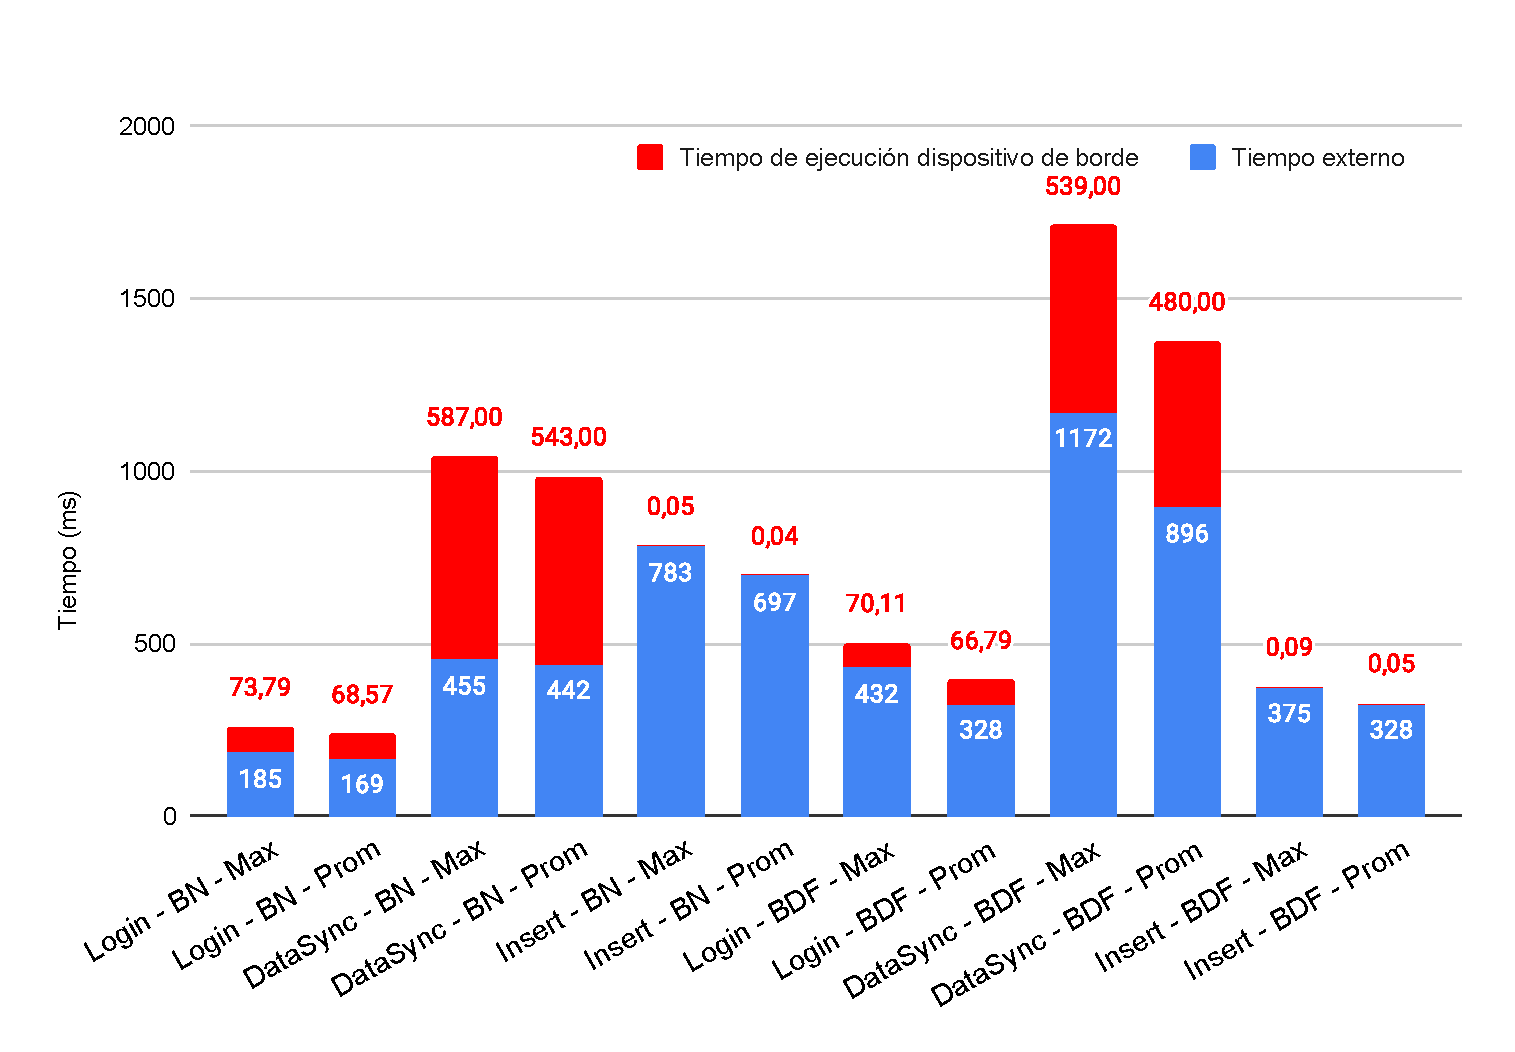
\includegraphics[width=\textwidth]{Imagenes/Experimentos/experimentoBarrasOperaciones.pdf}
        \caption{Evaluación inicial}
        \label{fig:evaluacionInicial}
\end{figure}

\section{Conectividad entre dispositivos}
\label{sec:conectividadDispositivos}
Con este experimento se busca someter a un dispositivo de niebla a una prueba de estrés ante múltiples conexiones y solicitudes concurrentes. Para ello se conectan hasta 64 dispositivos de borde de manera simultánea e incremental. Cada dispositivo de borde es emulado a través de un \textit{script} y se encuentra conectado a la misma red de área local que un dispositivo de niebla. Se simula una situación de pérdida de conectividad con la nube, por lo que no hay conexión con ella. Se realizan dos tipos de prueba diferentes:
\begin{itemize}
    \item \textbf{Prueba continua (PC):} Cada dispositivo de borde hace un \textit{insert}. Al hacerlo, como respuesta, recibe un mensaje de ``Ok'' y posteriormente un \textit{copy}, solo al recibir el \textit{copy}, un dispositivo de borde comienza a enviar otra solicitud de \textit{insert}.
    \item \textbf{Prueba periódica (PP):} Cada dispositivo de borde hace un \textit{insert} cada 30 segundos independientemente de si llega o no un \textit{copy}.
\end{itemize}

En ambos tipos de pruebas los tiempos medidos corresponden al intervalo entre el inicio de la operación de \textit{insert} y la recepción del \textit{copy} correspondiente. Durante todo el proceso, no se produjeron desconexiones ni se presentaron problemas relacionados con la red o con el dispositivo de niebla encargado de procesar la información.
 
El sistema se comportó correctamente en ambos tipos de pruebas. En la prueba continua (PC), se observó un tiempo promedio aproximado de 9570 ms para 64 dispositivos, 5140 ms para 32 dispositivos y 2280 ms para 16 dispositivos. También se realizaron pruebas con menos dispositivos, cuyos resultados se representan en la Figura \ref{fig:tiemposPromediosPruebas}. La diferencia en los tiempos es notable debido al crecimiento exponencial en la cantidad de mensajes de respuesta, lo que implica una mayor carga de cómputo sobre el dispositivo de niebla. Por ejemplo, si se utilizan 4 dispositivos de borde y cada uno realiza 4 \textit{inserts}, cada operación de \textit{insert} genera 4 operaciones de respuesta (\textit{copy}), lo que implica 16 mensajes de (\textit{copy}) en total, una para cada dispositivo de borde. Si se agregara otro dispositivo más, se tendría un total de 25 mensajes \textit{copy}.

En cuanto a los tiempos máximos en la prueba continua (PC), el sistema mantuvo un comportamiento adecuado y consistente a lo visto para los tiempos medios, registrando 12820 ms para 64 dispositivos, 5950 ms para 32 dispositivos y 2735 ms para 16 dispositivos, representados en la Figura \ref{fig:tiemposMaximosPruebas}.

En la prueba periódica (PP), se observó un tiempo medio de 5230 ms para 64 dispositivos, 2400 ms para 32 dispositivos y 1110 ms para 16 dispositivos. La diferencia de tiempos respecto a la prueba continua (PC) se debe a que el dispositivo de niebla tiene menos carga, esto se debe a que las operaciones \textit{insert} se realizan cada 30 segundos. En la Figura \ref{fig:tiemposPromediosPruebas} se muestra la comparativa de tiempos promedios para las diferentes cantidades de dispositivos.

En los tiempos máximos de la prueba periódica, el sistema también mostró un comportamiento adecuado y consistente, registrando 10775 ms para 64 dispositivos, 4715 ms para 32 dispositivos y 2140 ms para 16 dispositivos, como se muestra en la Figura \ref{fig:tiemposMaximosPruebas}.

\begin{figure}
    \centering
    \begin{minipage}{.8\textwidth}
        \centering
        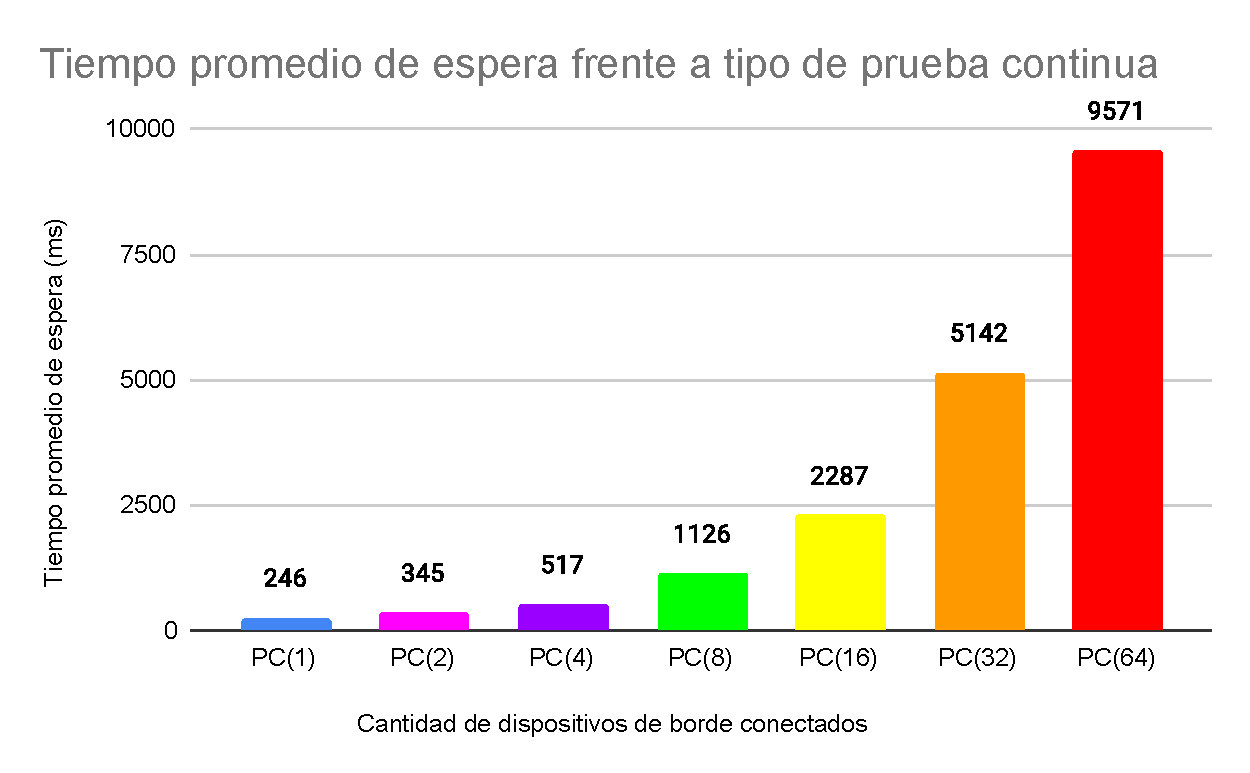
\includegraphics[width=\textwidth]{Imagenes/Experimentos/Tiempo promedio de espera frente a tipo de prueba continua.pdf}
    \end{minipage}%
    \hfill
    \begin{minipage}{.8\textwidth}
        \centering
        \includegraphics[width=\textwidth]{Imagenes/Experimentos/Tiempo promedio de espera frente a tipo de prueba periódica.pdf}
    \end{minipage}%
   
    \caption{Tiempos promedios de prueba continua y periódica}
    \label{fig:tiemposPromediosPruebas}
\end{figure}



\begin{figure}
    \centering
    \begin{minipage}{.8\textwidth}
        \centering
        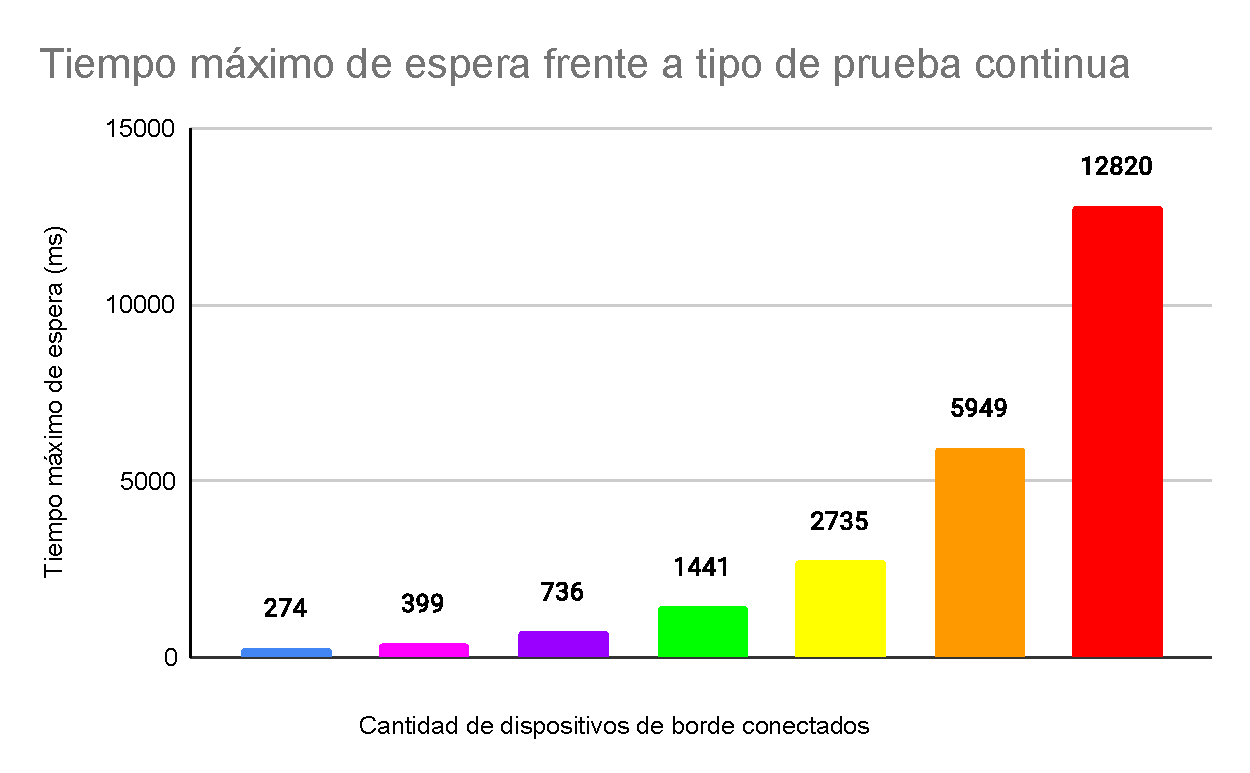
\includegraphics[width=\textwidth]{Imagenes/Experimentos/Tiempo maximo de espera frente a tipo de prueba continua.pdf}
    \end{minipage}%
    \hfill
    \begin{minipage}{.8\textwidth}
        \centering
        \includegraphics[width=\textwidth]{Imagenes/Experimentos/Tiempo maximo de espera frente a tipo de prueba periódica.pdf}
    \end{minipage}%
   
    \caption{Tiempos máximos de prueba continua y periódica}
    \label{fig:tiemposMaximosPruebas}
\end{figure}

A partir de los resultados observados y el análisis planteado se demuestra que la implementación del núcleo del sistema ALERTAR funciona exitosamente ante situaciones de alta carga con operaciones concurrentes sobre los dispositivos de niebla. Asegurando la consistencia y persistencia de los datos además de demostrar una alta capacidad de resiliencia ante eventos de falta de conectividad con servidores externos como lo es la nube.
\chapter{Conclusiones y trabajos futuros}
\label{cap:conclusionesYTrabajosFuturos}

El objetivo de este trabajo de tesis era implementar un prototipo básico del núcleo de la aplicación móvil del sistema ALERTAR compuesto por una plataforma base y un conjunto limitado de casos de uso implementados sobre ella, exceptuando la interfaz gráfica. 

En primer lugar, se implementó con éxito la capa de transporte de la aplicación móvil, asegurando la protección de la información confidencial de pacientes a través de comunicaciones seguras. Durante la implementación se desarrolló un manejador de mensajes discretos para su envío y recepción. Además, fue necesario implementar un mecanismo de detección de pérdida de conectividad debido a problemas presentados por la biblioteca utilizada para establecer transmisiones \textit{TLS/TCP}. Para garantizar las comunicaciones seguras se implementó un mecanismo de autenticación de dispositivos junto con un sistema de distribución de certificados digitales. Todo el desarrollo se realizó asegurando la serialización de las operaciones, a fin de evitar errores o estados inconsistentes, garantizando así que las operaciones se procesan en el mismo orden en el llegan al dispositivo encargado de ello.

En segundo lugar, se implementó un mecanismo de tolerancia a fallos basado en la replicación de datos entre dispositivos móviles y la nube. Para esto, se utilizó una arquitectura limpia la cual contempla la implementación de servicios para la comunicación de los diferentes dispositivos del sistema, la implementación de una base de datos y la implementación de casos de uso encargados de ejecutar funcionalidades del sistema. Con esto se abarcaron aspectos como seguridad, modularidad y escalabilidad, dando como resultado un código escalable y de fácil modificación. Además, se realizó una especificación del sistema, la cual incluye un diagrama de la arquitectura limpia utilizada, un diagrama de casos de uso y diagramas de actividades que explican el funcionamiento de los casos de uso implementados más significativos. También se incorporó un ejemplo de diagrama de clases, a fin de retratar cómo está implementada la arquitectura limpia.

En tercer lugar, se verificó el correcto funcionamiento del mecanismo de tolerancia a fallos. Se contemplaron los diferentes tipos de conexión que pueden existir en el sistema y se realizó una validación funcional con casos de usos implementados, la cual verificó el correcto funcionamiento del sistema así como su capacidad de recuperación ante los diferentes tipos de fallos posibles. Se desarrollaron interfaces gráficas para poder ejecutar diferentes casos de uso y procedimientos y así poder evaluar su funcionamiento durante el desarrollo. Además, se realizó una prueba de concurrencia en dispositivos de niebla para evaluar su capacidad para trabajar con múltiples conexiones simultáneas a través de una red de área local desde dispositivos de borde.

Por último, se realizó una evaluación del rendimiento de la aplicación móvil implementada, considerando eficiencia del almacenamiento local de datos y tiempo de ejecución de operaciones básicas del mecanismo de tolerancia a fallos basado en replicación de datos. Obteniendo resultados satisfactorios en ambas pruebas. 



Todo este trabajo derivó en la validación de la plataforma base e identificación de posibles mejoras arquitectónicas o de implementación. El desarrollo de este prototipo representa un paso significativo hacia la creación de la aplicación móvil del sistema ALERTAR. Las funcionalidades implementadas permiten garantizar comunicaciones seguras, tolerancia a fallos y operación autónoma sin dependencia constante de Internet o disponibilidad de servicios en la nube. Estas capacidades son fundamentales para mejorar la calidad y continuidad de la atención médica en hospitales con recursos tecnológicos reducidos, ofreciendo una herramienta concreta para salvar vidas en entornos críticos.
\section{Trabajos futuros}

Como continuación de este trabajo de tesis se sugieren los siguientes trabajos futuros:
\begin{itemize}
    \item Implementar mecanismos de seguridad para los datos almacenados en memoria secundaria de los dispositivos móviles.
    \item Agregar datos de manera automática a partir de la información proporcionada por sensores u otro equipamiento médico.
    \item Aplicar un sistema de compresión de datos.
    \item Paginar mensajes de capa de aplicación cuando son demasiado grandes para evitar desbordamientos de buffer.
    \item Aplicar distinciones en los casos de uso en función de si el usuario pertenece al personal médico o de enfermería.
    \item Investigar cómo ejecutar la aplicación en segundo plano sin que se pierda la conexión con
    los dispositivos de niebla, y que estos sigan operativos, en el caso de que un usuario la pase a segundo plano.
\end{itemize}



\vfill
\pagebreak
\nocite{*}
%\chapter{Referencias bibliográficas}
%\renewcommand{\refname}{Referencias bibliográficas}
\label{sec:org6b525e0}
\addcontentsline{toc}{chapter}{Referencias Bibliográficas}
\printbibliography[% heading=none,
title={Referencias Bibliográficas}]


%%Si hubiera apéndices:
\appendix
\chapter{Especificación de casos de uso}
\label{Anexo: Especificacion}
\begin{figure}
    \centering
    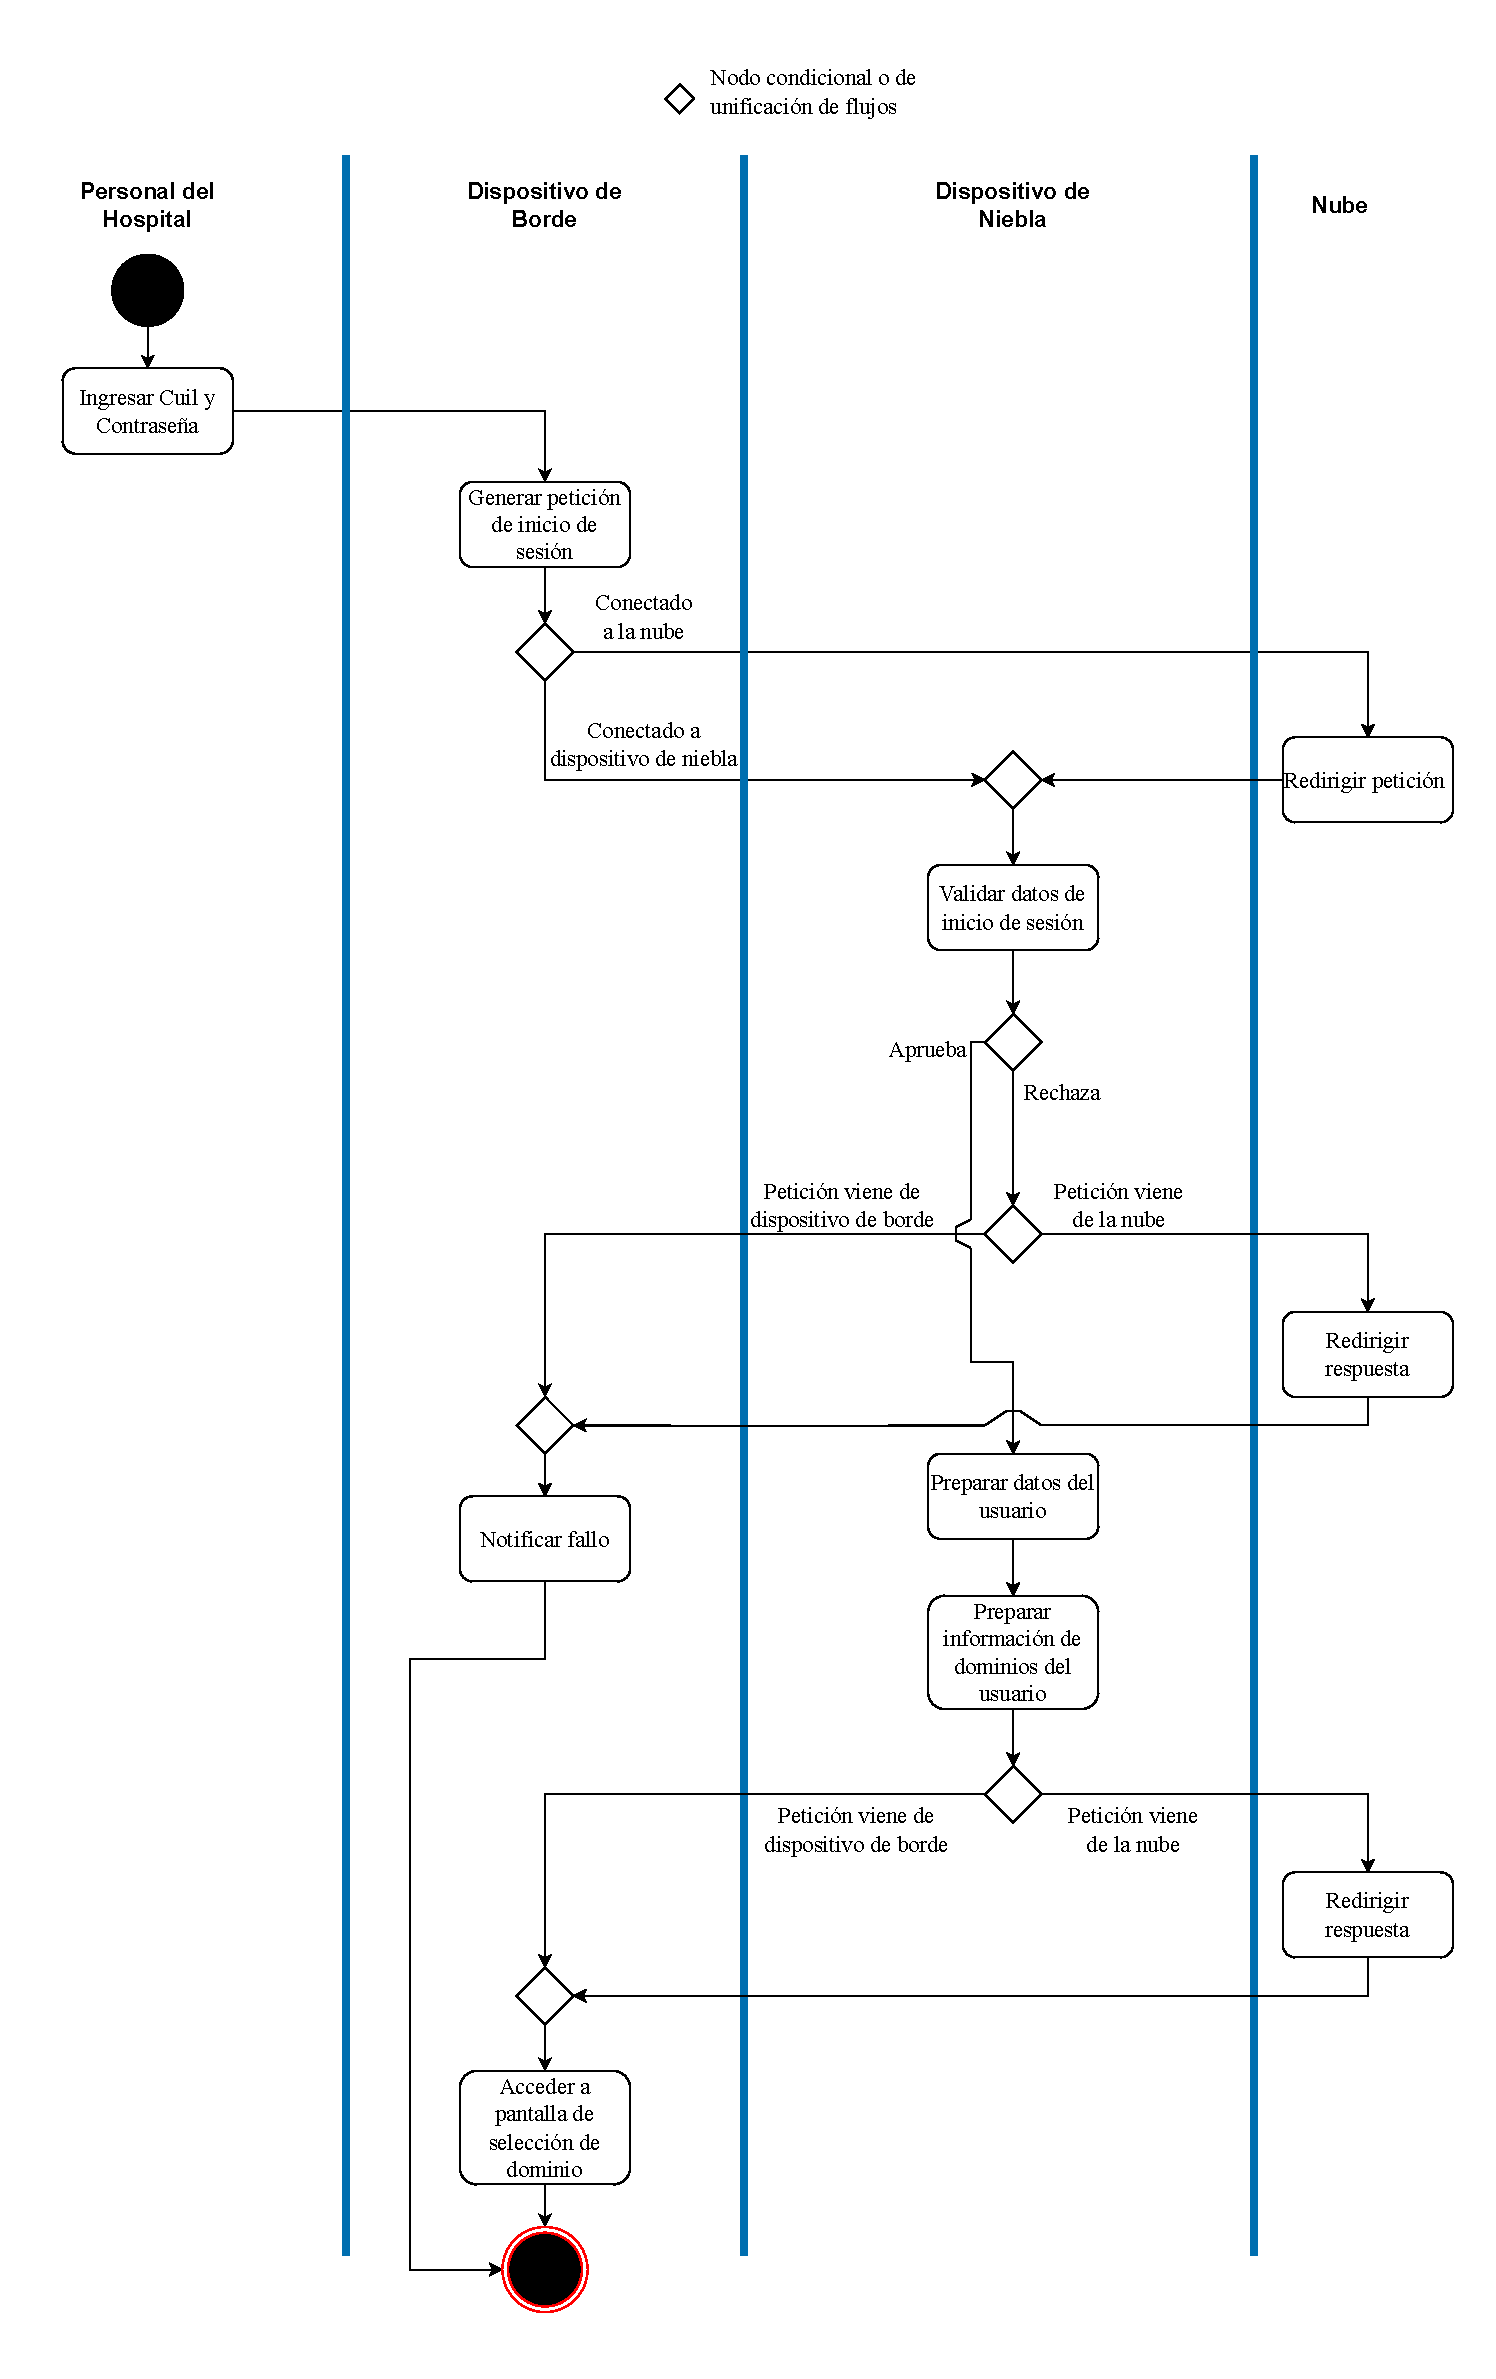
\includegraphics[height=\textheight, keepaspectratio]{Imagenes/Implementacion/IniciarSesionDA.pdf}
    \caption{Diagrama de actividades del caso de uso \textit{Iniciar Sesión}}
    \label{fig:diagActIniciarSesion}
\end{figure}




\begin{figure}
    \centering
    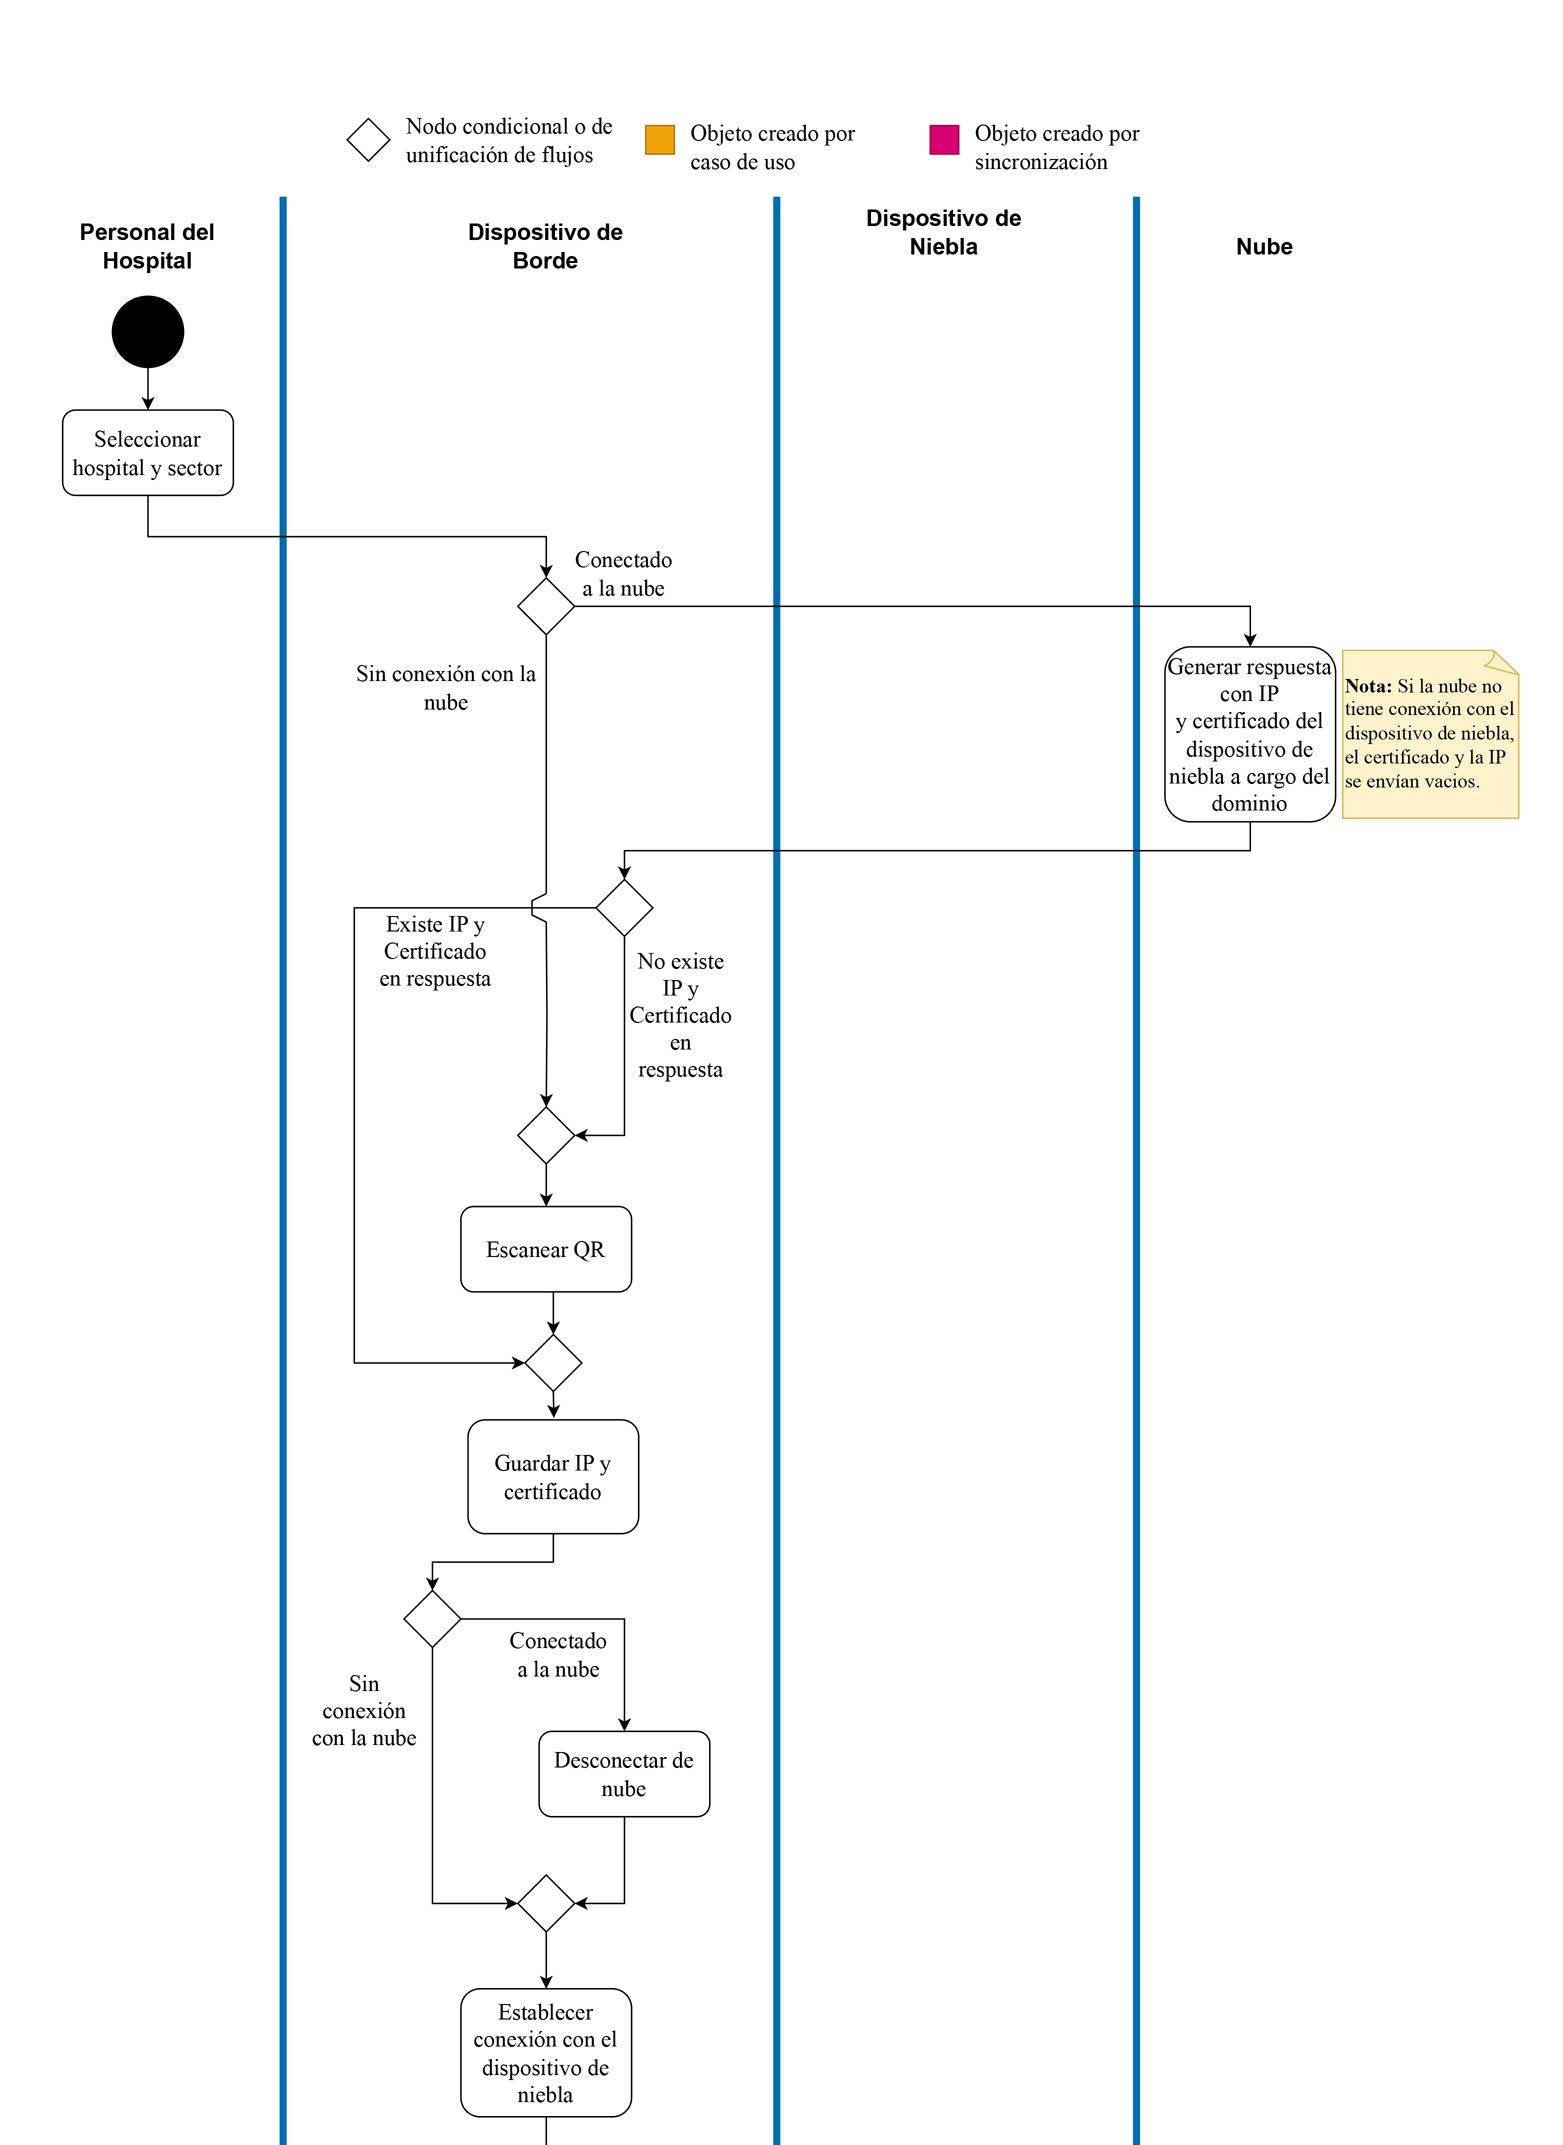
\includegraphics[width=\textwidth, height=\textheight, keepaspectratio]{Imagenes/Implementacion/ConectarseDominioDA1.pdf}
    \caption{Diagrama de actividades del caso de uso \textit{Conectarse a dominio} primer mitad}
    \label{fig:diagActConectDom}
\end{figure}

\begin{figure}
    \centering
    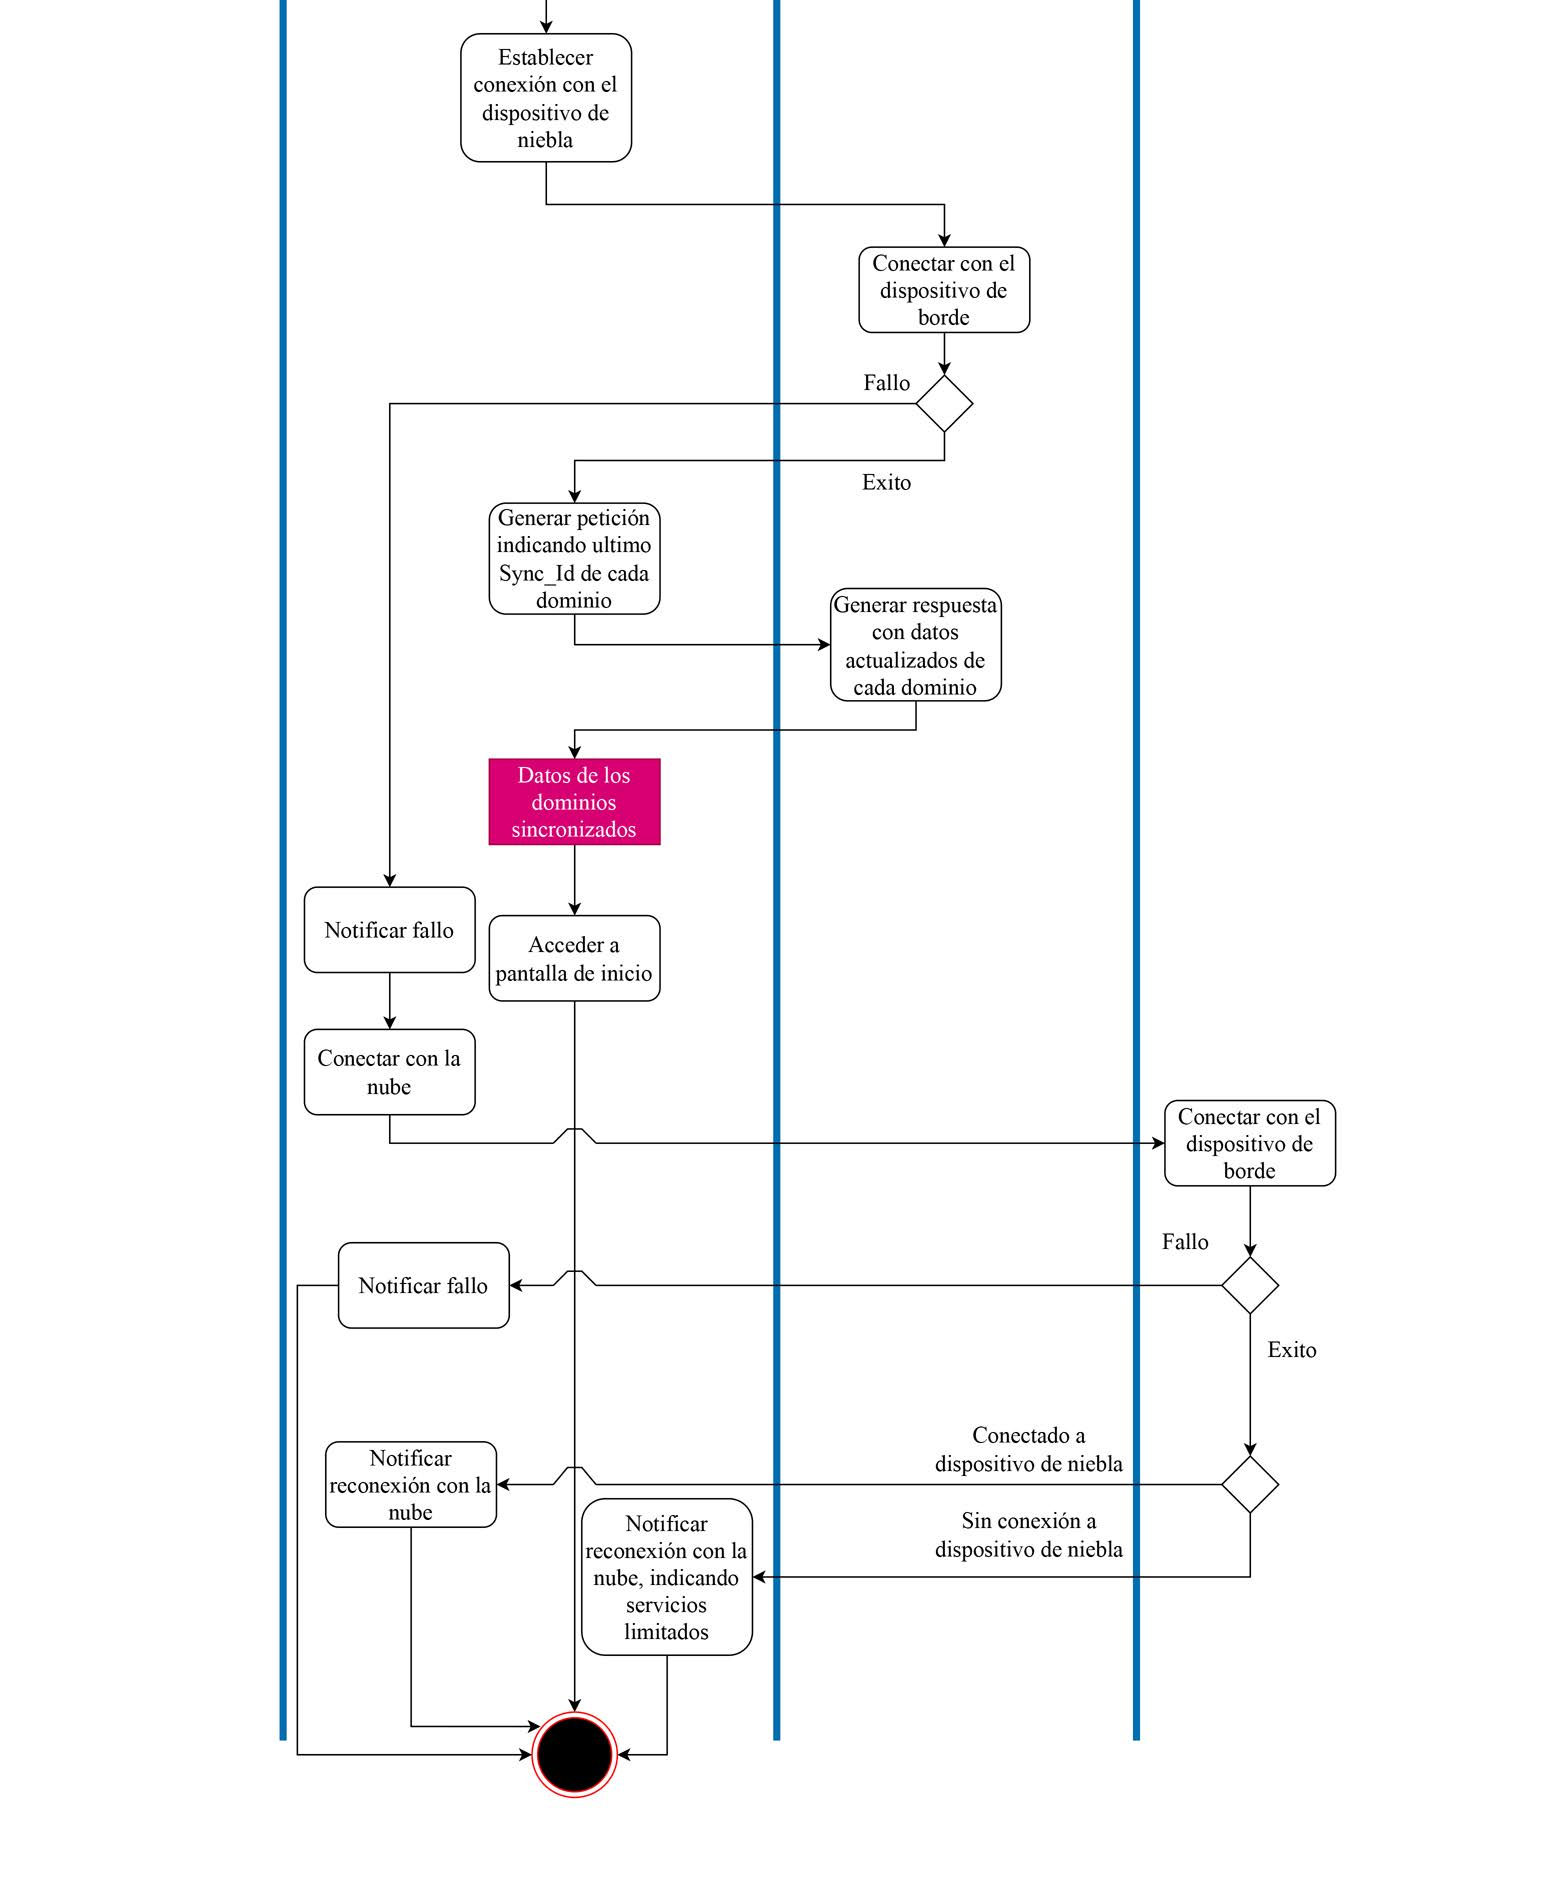
\includegraphics[width=\textwidth, height=\textheight, keepaspectratio]{Imagenes/Implementacion/ConectarseDominioDA2.pdf}
    \caption{Diagrama de actividades del caso de uso \textit{Conectarse a dominio} segunda mitad}
    \label{fig:diagActConectDom2}
\end{figure}

%\begin{figure}
%    \centering
    %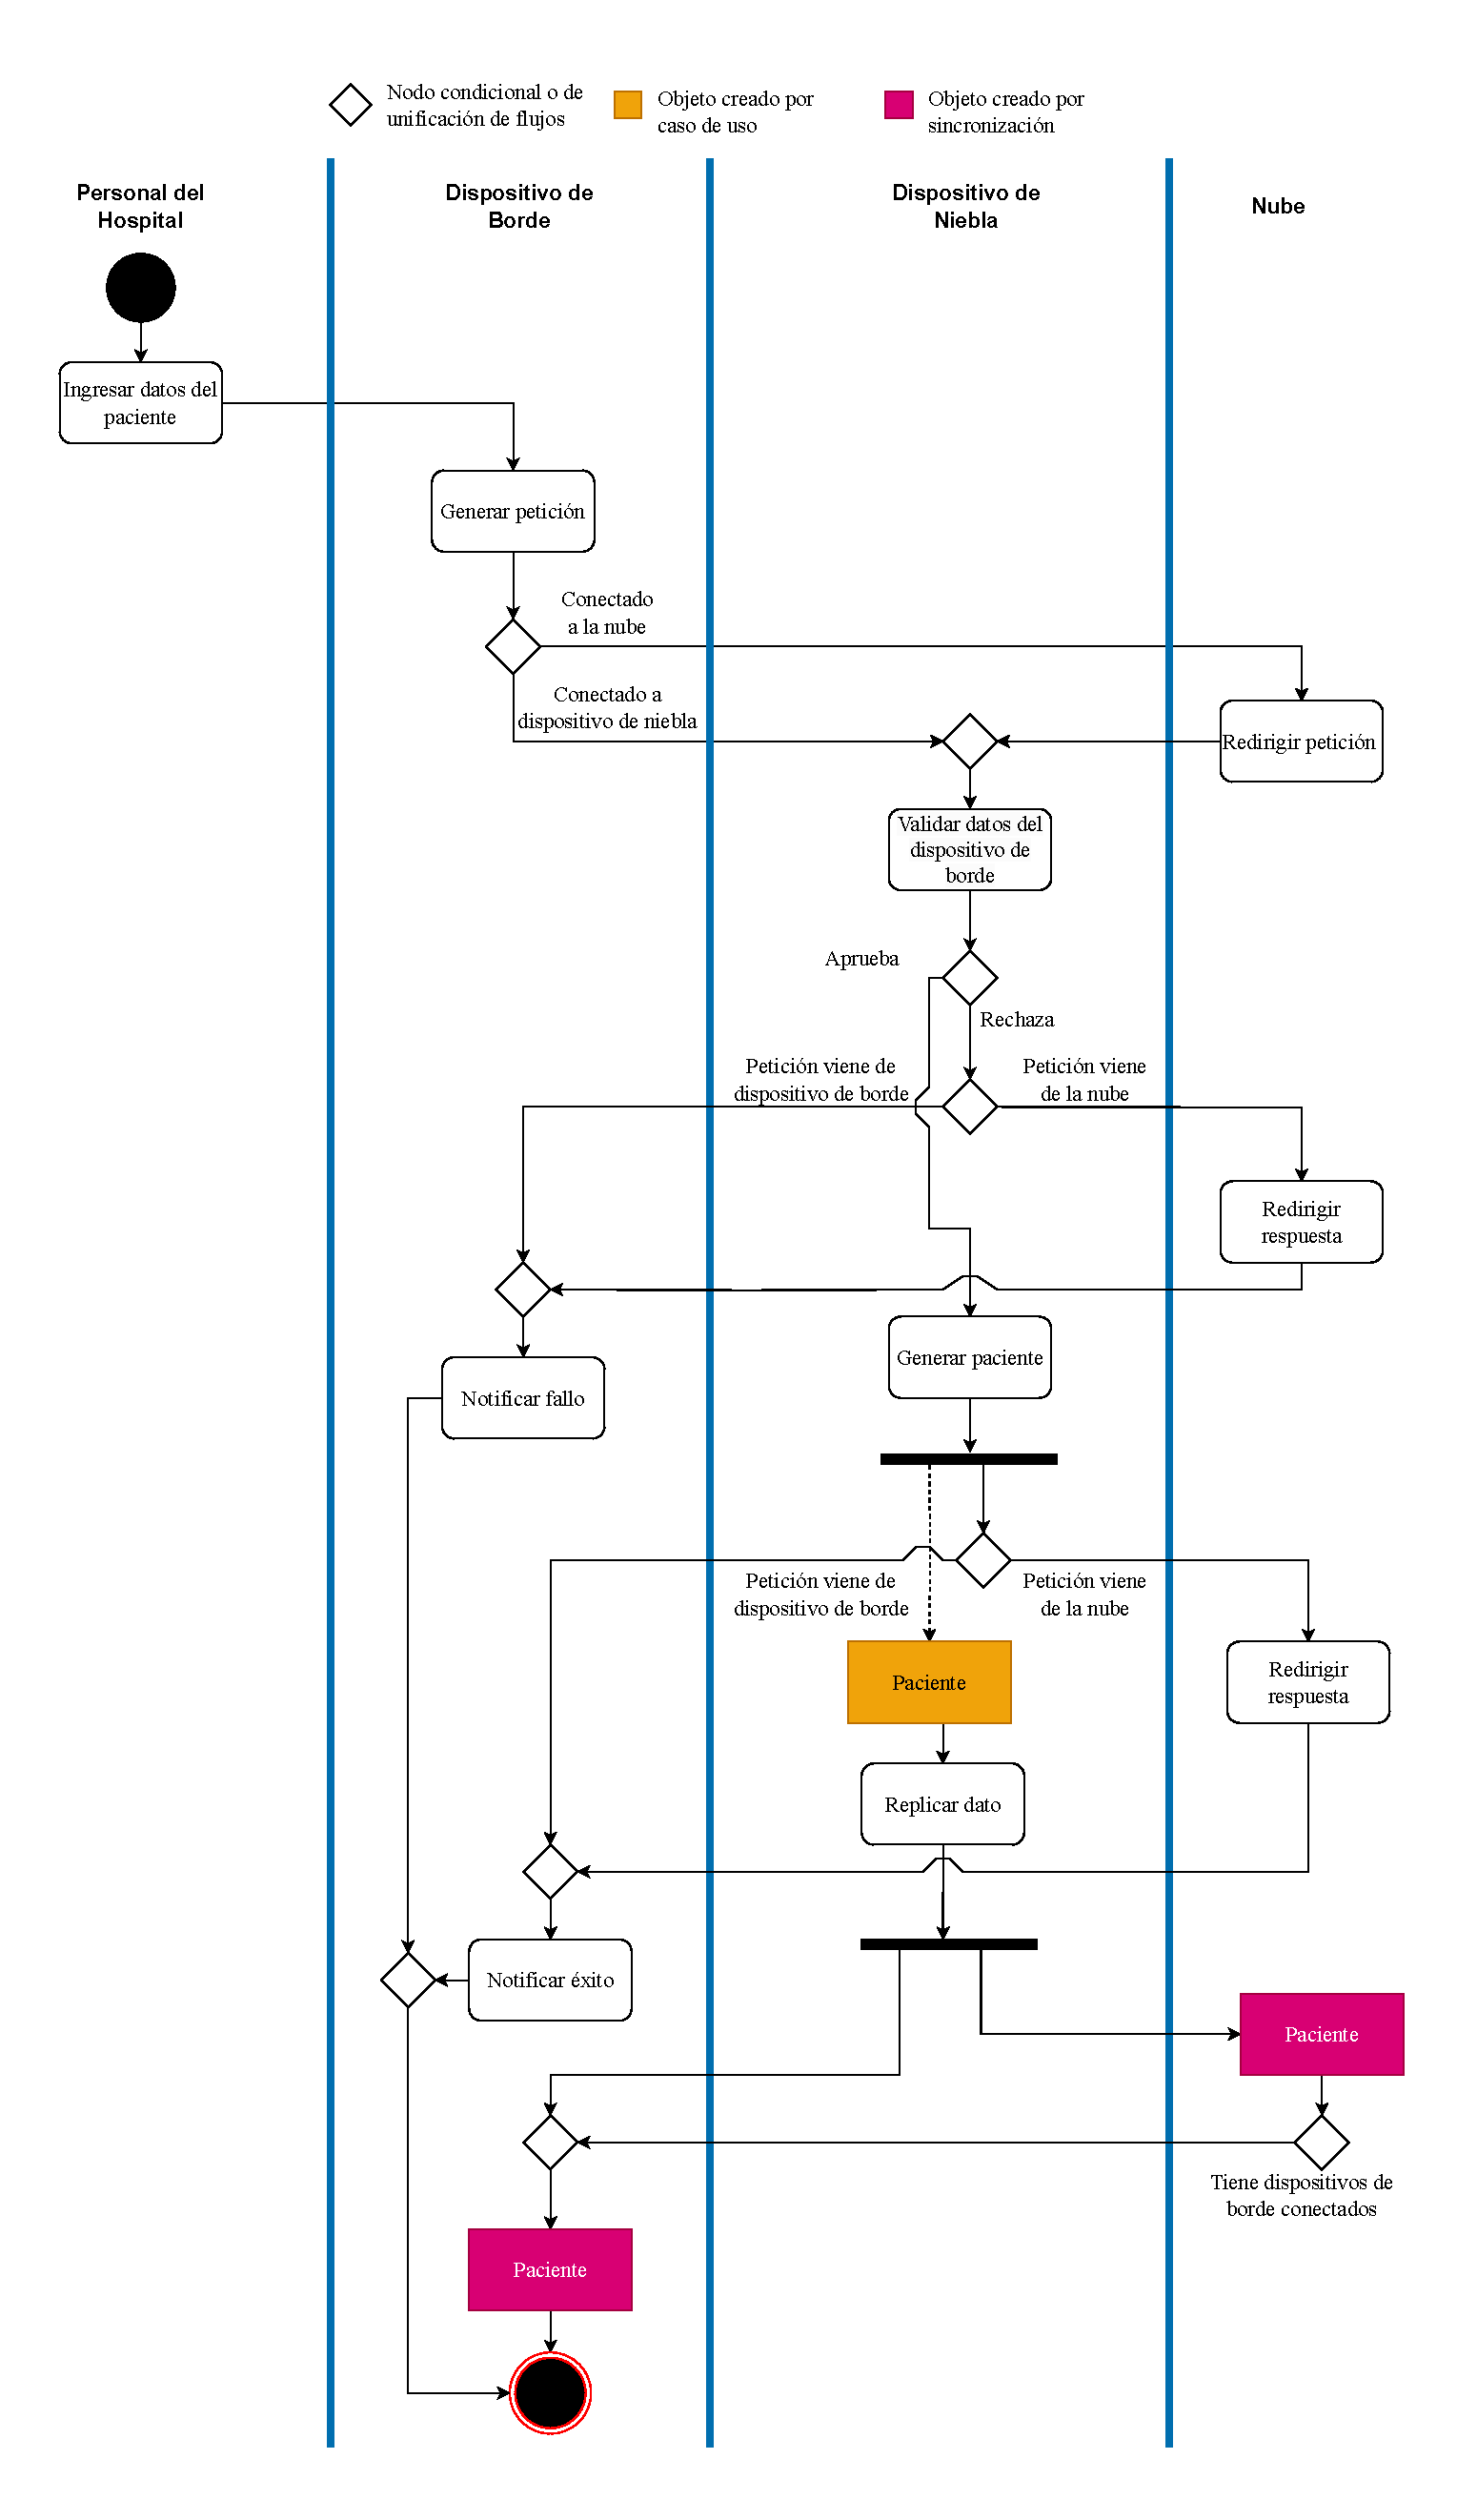
\includegraphics[width=\textwidth, height=\textheight, keepaspectratio]{Imagenes/Implementacion/IngresarPacienteDA.pdf}
    %\caption{Diagrama de actividades del caso de uso \textit{Admisión paciente}}
    %\label{fig:diagActIngresarPaciente}
%\end{figure}

\begin{figure}
    \centering
    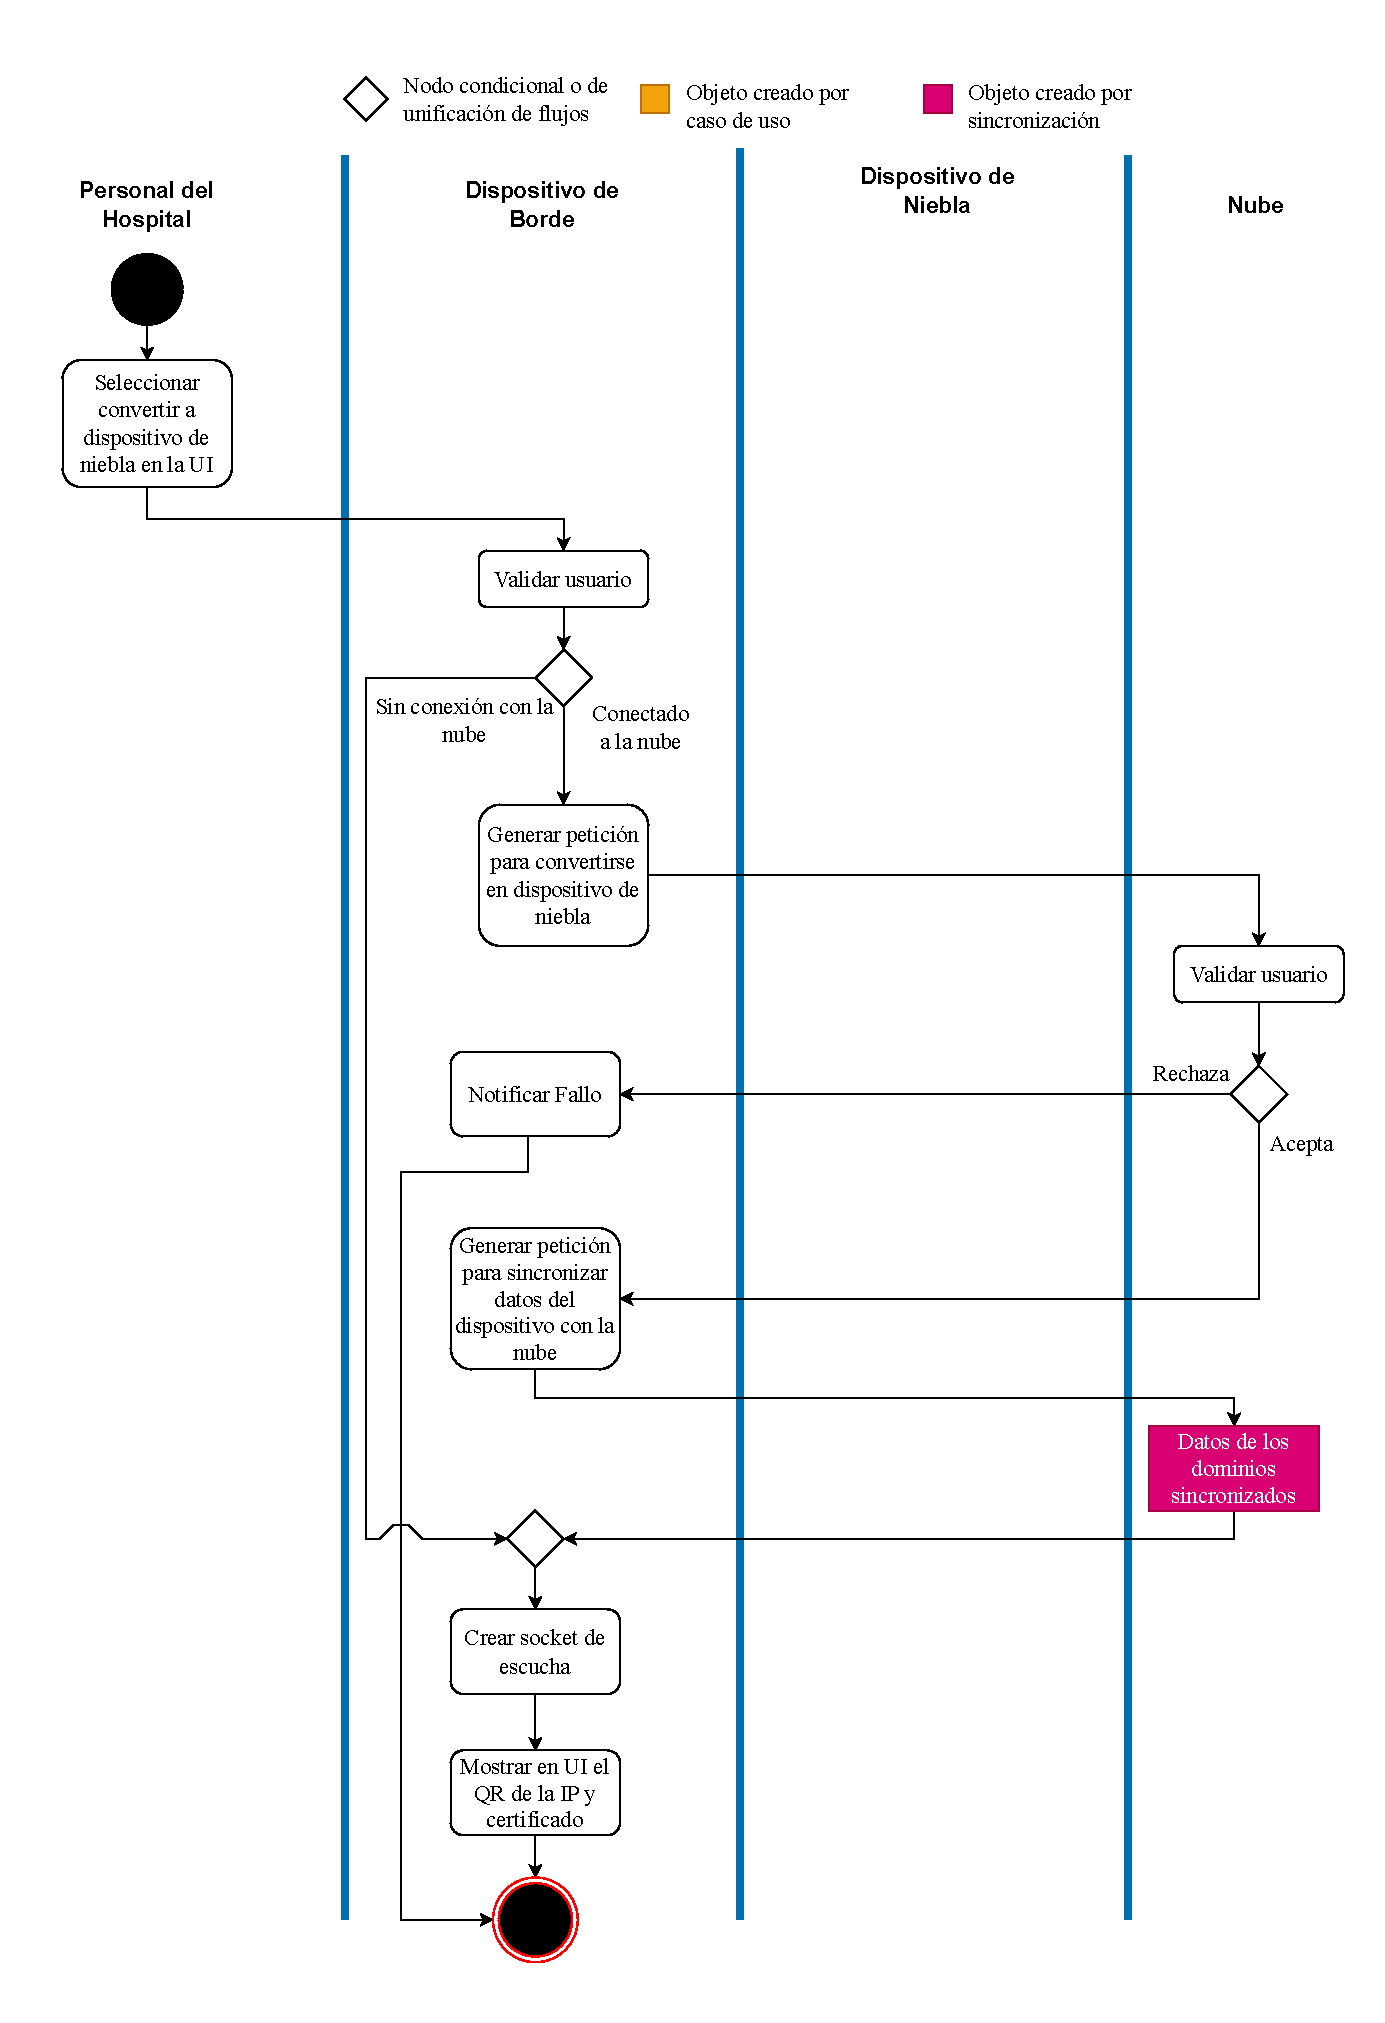
\includegraphics[width=\textwidth, height=\textheight, keepaspectratio]{Imagenes/Implementacion/ConvertirALiderDA.pdf}
    \caption{Diagrama de actividades del caso de uso \textit{Convertir a dispositivo de niebla}}
    \label{fig:diagActConvertALider}
\end{figure}


\chapter{Tabla de resultados de los experimentos}
\begin{table}[h]
\centering
\begin{tabular}{|l|p{4cm}|p{4cm}|c|}
\hline
\textbf{Cantidad de registros} & \textbf{Tamaño total requerido (bytes)} & \textbf{Tamaño real medido (bytes)} & \textbf{Sobrecarga \%} \\ \hline
100 & 13,600 & 188,416 & 1285.41\% \\ \hline
200 & 27,200 & 212,992 & 683.06\% \\ \hline
300 & 40,800 & 229,376 & 462.20\% \\ \hline
400 & 54,400 & 249,856 & 359.29\% \\ \hline
500 & 68,000 & 270,336 & 297.55\% \\ \hline
600 & 81,600 & 286,720 & 251.37\% \\ \hline
700 & 95,200 & 303,104 & 218.39\% \\ \hline
800 & 108,800 & 323,584 & 197.41\% \\ \hline
900 & 122,400 & 344,064 & 181.10\% \\ \hline
1000 & 136,000 & 364,544 & 168.05\% \\ \hline
1100 & 149,600 & 385,024 & 157.37\% \\ \hline
1200 & 163,200 & 397,312 & 143.45\% \\ \hline
1300 & 176,800 & 417,792 & 136.31\% \\ \hline
1400 & 190,400 & 438,272 & 130.18\% \\ \hline
1500 & 204,000 & 458,752 & 124.88\% \\ \hline
1600 & 217,600 & 475,136 & 118.35\% \\ \hline
1700 & 231,200 & 495,616 & 114.37\% \\ \hline
1800 & 244,800 & 516,096 & 110.82\% \\ \hline
1900 & 258,400 & 532,480 & 106.07\% \\ \hline
2000 & 272,000 & 552,960 & 103.29\% \\ \hline
2100 & 285,600 & 569,344 & 99.35\% \\ \hline
2200 & 299,200 & 589,824 & 97.13\% \\ \hline
2300 & 312,800 & 610,304 & 95.11\% \\ \hline
2400 & 326,400 & 630,784 & 93.25\% \\ \hline
2500 & 340,000 & 643,072 & 89.14\% \\ \hline
2600 & 353,600 & 663,552 & 87.66\% \\ \hline
2700 & 367,200 & 684,032 & 86.28\% \\ \hline
2800 & 380,800 & 704,512 & 85.01\% \\ \hline
2900 & 394,400 & 720,896 & 82.78\% \\ \hline
3000 & 408,000 & 741,376 & 81.71\% \\ \hline
\end{tabular}
\caption{Tamaño total requerido, tamaño real medido y sobrecarga de los registros (solo con registros tipo Paciente insertados)}
\label{tabla:TamReqYRealConOverPacientes}
\end{table}

\begin{table}[h]
\centering
\begin{tabular}{|l|p{4cm}|p{4cm}|c|}
\hline
\textbf{Cantidad de registros} & \textbf{Tamaño total requerido (bytes)} & \textbf{Tamaño real medido (bytes)} & \textbf{Sobrecarga \%} \\ \hline

3100 & 421,600 & 761,856 & 80.71\% \\ \hline
3200 & 435,200 & 778,240 & 78.82\% \\ \hline
3300 & 448,800 & 798,720 & 77.97\% \\ \hline
3400 & 462,400 & 815,104 & 76.28\% \\ \hline
3500 & 476,000 & 835,584 & 75.54\% \\ \hline
3600 & 489,600 & 856,064 & 74.85\% \\ \hline
3700 & 503,200 & 876,544 & 74.19\% \\ \hline
3800 & 516,800 & 888,832 & 71.99\% \\ \hline
3900 & 530,400 & 909,312 & 71.44\% \\ \hline
4000 & 544,000 & 929,792 & 70.92\% \\ \hline
4100 & 180,400 & 929,792 & 415.41\% \\ \hline
4200 & 184,800 & 946,176 & 412.00\% \\ \hline
4300 & 189,200 & 946,176 & 400.09\% \\ \hline
4400 & 193,600 & 954,368 & 392.96\% \\ \hline
4500 & 198,000 & 962,560 & 386.14\% \\ \hline
4600 & 202,400 & 978,944 & 383.67\% \\ \hline
4700 & 206,800 & 983,040 & 375.36\% \\ \hline
4800 & 211,200 & 991,232 & 369.33\% \\ \hline
4900 & 215,600 & 999,424 & 363.55\% \\ \hline
5000 & 220,000 & 1,007,616 & 358.01\% \\ \hline
5100 & 224,400 & 1,015,808 & 352.68\% \\ \hline
5200 & 228,800 & 1,028,096 & 349.34\% \\ \hline
5300 & 233,200 & 1,036,288 & 344.38\% \\ \hline
5400 & 237,600 & 1,044,480 & 339.60\% \\ \hline
5500 & 242,000 & 1,048,576 & 333.30\% \\ \hline
5600 & 246,400 & 1,056,768 & 328.88\% \\ \hline
5700 & 250,800 & 1,064,960 & 324.63\% \\ \hline
5800 & 255,200 & 1,069,056 & 318.91\% \\ \hline
5900 & 259,600 & 1,077,248 & 314.96\% \\ \hline
6000 & 264,000 & 1,081,344 & 309.60\% \\ \hline
\end{tabular}
\caption{Tamaño total requerido, tamaño real medido y sobrecarga de los registros (a los registros pacientes ingresados se le agregaron los registros Cama)}
\label{tabla:TamReqYRealConOverCamas}
\end{table}

\end{document}
